% Wrapper για τη μεταγλώττιση της πλήρους διπλωματικής εργασίας.
%
% Αντιστοίχιση κεφαλαίων:
%   Κεφάλαιο 1 (Εισαγωγή)                        -> chapter_introduction.tex
%   Κεφάλαιο 2 (Θεωρητικό Υπόβαθρο)              -> chapter_background.tex
%   Κεφάλαιο 3 (Αλγόριθμοι)                       -> chapter_algorithms.tex
%   Κεφάλαια 4-6 (Ρύθμιση, Αποτελέσματα, Σύγκριση) -> chapter_experiments.tex
%   Κεφάλαιο 7 (Συμπεράσματα)                     -> chapter_conclusions.tex
%   Παράρτημα                                      -> appendix.tex
%
\documentclass[11pt,a4paper]{report}

% XeLaTeX preamble for Greek Unicode support
\usepackage[margin=1in]{geometry}
\usepackage{float}
\usepackage{amsmath, amssymb}
\usepackage{booktabs}
\usepackage{array}
\usepackage{graphicx}
\usepackage{subcaption}
\usepackage{hyperref}
\usepackage{algorithm}
\usepackage{algpseudocode}
\usepackage{natbib}

\usepackage[utf8]{inputenc}
\usepackage[T1]{fontenc}
\usepackage[greek,english]{babel}
\usepackage{alphabeta}
\DeclareGraphicsExtensions{.pdf,.png,.jpg}

% Ελληνικές επικεφαλίδες για κεφάλαια, πίνακα περιεχομένων και περίληψη.
% Πρέπει να μπουν στο hook του babel, αλλιώς το babel τις επαναφέρει στα αγγλικά
% κατά το \begin{document} (η κύρια γλώσσα είναι η english). Τα ορίζουμε και για
% τις δύο γλώσσες ώστε να ισχύουν όποια κι αν είναι η ενεργή.
\addto\captionsenglish{%
    \renewcommand{\chaptername}{Κεφάλαιο}%
    \renewcommand{\contentsname}{Περιεχόμενα}%
    \renewcommand{\abstractname}{Περίληψη}%
    \renewcommand{\bibname}{Βιβλιογραφία}%
    \renewcommand{\appendixname}{Παράρτημα}%
  }
  \addto\captionsgreek{%
    \renewcommand{\chaptername}{Κεφάλαιο}%
    \renewcommand{\contentsname}{Περιεχόμενα}%
    \renewcommand{\abstractname}{Περίληψη}%
    \renewcommand{\bibname}{Βιβλιογραφία}%
    \renewcommand{\appendixname}{Παράρτημα}%
  }


\bibliographystyle{plainnat}

%
%\title{Σύγκριση Αλγορίθμων Langevin σε %Κατανομές Ποικίλης Βαρύτητας Ουράς}
%\author{Χρήστος Πλασκασοβίτης}
%\date{}

\begin{document}
\include{thesis/thesis_greek/cover}

%\maketitle

\begin{abstract}
\noindent
Η παρούσα εργασία παρουσιάζει μία πειραματική σύγκριση τριών δειγματοληπτών από την οικογένεια Langevin σε ένα ελεγχόμενο εύρος κατανομών-στόχων και
διαστάσεων. Άρχικα παρουσιάζονται δύο overdamped εκδοχές, ο Unadjusted Langevin
Algorithm (ULA) που είναι η βασικότερη μορφή των langevin δειγματοληπτών και ο Metropolis-Adjusted Langevin Algorithm (MALA) ο οποίος επεκτίνει τον ULA εισάγοντας ένα metropolis rejection step. Επίσης διερευνάται και μια underdamped εκδοχή, ο kinetic langevin ο οποίος υλοποιείται μεσώ ενος BAOAB splitting ολοκληρωτή. Οι κατανομές-στόχοι πάνω στις οποίες γίνεται η σύγκριση των αλγορίθμων είναι μια τυπική Γκαουσιανή (ελαφριές,
εκθετικές ουρές), μια κατανομή Student-$t$ με πέντε βαθμούς ελευθερίας (μέτριες
πολυωνυμικές ουρές με πεπερασμένη διακύμανση) και μια τυπική κατανομή Cauchy
(ακραίες πολυωνυμικές ουρές χωρίς πεπερασμένες ροπές). 

Για κάθε αλγόριθμο και κατανομή στόχο διενεργείται μια σειρά πειραμάτων δειγματοληψίας στα οποία εναλλάσονται διάφορες παράμετροι όπως το βήμα (step size), ο αριθμός των διαστάσεων και η τριβή (στον kinetic). Για κάθε πείραμα διενεργούνται $20$
ανεξάρτητες εκτελέσεις με τυχαία αρχική κατάσταση. Συνολικά μελετώνται περίπου $10{,}000$ αλυσίδες. Για την αξιολόγηση και την σύγκριση των αλγορίθμων χρησιμοποιείται μια σειρά διαγνωστικών--στατιστικών. Τα διαγνωστικά περιλαμβάνουν το αποτελεσματικό μέγεθος δείγματος (ESS), το στατιστικό Kolmogorov--Smirnov (KS statistic) έναντι της αναλυτικής περιθώριας κατανομής, το μέσο απόλυτο σφάλμα ποσοστημορίου (q-MAE) σε ακραία ποσοστημόρια και τους λόγους κάλυψης ουράς (tail coverage) κ.α.

Τα κύρια αποτελέσματα είναι τα εξής. Ο ULA παρουσιάζει μόνιμη
μεροληψία που δεν μειώνεται με τον αριθμό των επαναλήψεων: στην
κατανομή Cauchy, καμία από τις εκτελέσεις δεν κατάφερε να καλύψει
τα $1\%$ και $99\%$ ποσοστημόρια, και το σφάλμα ποσοστημορίου στο
$97.5\%$ αυξάνεται κατά δύο τάξεις μεγέθους σε σχέση με τη Γκαουσιανή.
Ο BAOAB δείχνει σταθερή συμπεριφορά ως προς τη διάσταση στη Γκαουσιανή,
με τιμές KS κοντά στο $0.006$ για $d \in [1, 100]$, κάτι που αναμένεται
θεωρητικά για το kinetic σχήμα και επιβεβαιώνεται εδώ εμπειρικά.
Και οι τρεις αλγόριθμοι αντιμετωπίζουν σοβαρές δυσκολίες στην
κατανομή Cauchy για $d \geq 50$: η μέση KS ξεπερνά το $0.5$ στο
$d=100$, οπότε η δειγματοληψία βαριών ουρών με $5 \times 10^4$
επαναλήψεις είναι ουσιαστικά αδύνατη. Σε χαμηλότερες διαστάσεις, ο
MALA είναι καλύτερος στην προσαρμογή του κύριου σώματος της κατανομής
(KS) ενώ ο BAOAB υπερέχει στην εκτίμηση ακραίων ποσοστημορίων (q-MAE),
οπότε η επιλογή μεταξύ τους εξαρτάται από τις ανάγκες της εκάστοτε δειγματοληψίας.
\end{abstract}

\tableofcontents

% !TEX root = main.tex
\chapter{Εισαγωγή}
\label{chap:introduction}

\section{Το Πρόβλημα Δειγματοληψίας σε Υψηλές Διαστάσεις}
\label{sec:intro-sampling}

Ένα κεντρικό ζήτημα στην υπολογιστική στατιστική, τη μηχανική μάθηση και τη
στατιστική φυσική είναι η παραγωγή δειγμάτων από μια κατανομή-στόχο πιθανότητας
$\pi$ στο $\mathbb{R}^d$ που είναι γνωστή μόνο έως μια σταθερά κανονικοποίησης.
Η συνήθης διατύπωση είναι να εκφραστεί η κατανομή-στόχος ως \emph{μέτρο Gibbs}
\begin{equation}
  \pi(x) \;\propto\; \exp(-U(x)), \qquad x \in \mathbb{R}^d,
  \label{eq:gibbs-intro}
\end{equation}
όπου $U : \mathbb{R}^d \to \mathbb{R}$ είναι μια συνάρτηση δυναμικού. 
\newline
Η άγνωστη σταθερά κανονικοποίησης $\int_{\mathbb{R}^d} \exp(-U(y))\, dy$ μπορεί να είναι
αδύνατο να υπολογιστεί (ιδιαίτερα σε υψηλές διαστάσεις), ωστόσο ένα ευρύ φάσμα ερωτημάτων στατιστικής
συμπερασματολογίας μπορεί να απαντηθεί αποκλειστικά από δείγματα: οι εκ των
υστέρων κατανομές στην Μπεϋζιανή στατιστική, οι ελεύθερες ενέργειες στη
στατιστική μηχανική, οι περιθώριες πιθανοφάνειες στην επιλογή μοντέλου ανάγονται όλα στον υπολογισμό του $\mathbb{E}_\pi[\varphi(X)]$ για κάποια συνάρτηση ελέγχου $\varphi$.

Σε χαμηλή διάσταση, γενικές μέθοδοι όπως το rejection ή το importance sampling λειτουργούν καλά. Καθώς η διάσταση αυξάνεται, ωστόσο,
αυτές οι μέθοδοι αποτυγχάνουν: ο όγκος του $\mathbb{R}^d$ εκρήγνυται ταχύτερα
από ό,τι μπορεί να καλύψει οποιοδήποτε σταθερό περίβλημα ή κατανομή πρότασης,
οπότε τα περισσότερα προτεινόμενα δείγματα είτε απορρίπτονται (στο rejection sampling) είτε λαμβάνουν βάρη σχεδόν μηδενικά (στο importance sampling), και η διακύμανση του εκτιμητή καθίσταται καταστροφική
\citep{robert2004monte}.

Η πιο διαδεδομένη προσέγγιση είναι το \emph{Markov chain Monte Carlo} (MCMC). Αντί να
παράγουμε ανεξάρτητα δείγματα, παράγουμε μια ενιαία ακολουθία
$(X_k)_{k\geq 0}$ \emph{εξαρτημένων} δειγμάτων, η οποία κατανέμεται
ασυμπτωτικά σύμφωνα με την $\pi$. Συγκεκριμένα, σχεδιάζουμε μια
αλυσίδα Markov της οποίας η μοναδική στάσιμη κατανομή είναι η $\pi$. Η εκτέλεσή
της για αρκετά μεγάλο χρόνο παράγει δείγματα που (αν και μη ανεξάρτητα)
συμπεριφέρονται ως τυχαίες επιλογές από την $\pi$ για τον σκοπό του υπολογισμού
προσδοκιών. Η μαθηματική εγγύηση που δικαιολογεί αυτό είναι το \emph{εργοδικό
θεώρημα}: υπό ήπιες συνθήκες, ο χρονικός μέσος $n^{-1}\sum_{k=1}^n \varphi(X_k)$
συγκλίνει στην προσδοκία $\mathbb{E}_\pi[\varphi(X)]$ καθώς $n \to \infty$
\citep{meyn2009markov, tierney1994markov}. Ο ρυθμός σύγκλισης εξαρτάται από τον
βαθμό συσχέτισης διαδοχικών δειγμάτων. Το καθιερωμένο μέτρο αυτού είναι το
\emph{αποτελεσματικό μέγεθος δείγματος} (ESS), που μετρά τον αριθμό των
πραγματικά ανεξάρτητων δειγμάτων σε μια συσχετισμένη αλυσίδα.

Η οικογένεια αλγορίθμων Langevin MCMC είναι από τις πιο εκτενώς μελετημένες και
ευρέως χρησιμοποιούμενες τεχνικές δειγματοληψίας \citep{roberts1996exponential, dalalyan2017theoretical, durmus2017nonasymptotic}. Κάθε αλγόριθμος αυτής της οικογένειας προκύπτει από τη
διακριτοποίηση μιας συνεχούς-χρόνου στοχαστικής διαφορικής εξίσωσης (SDE) της
οποίας το αναλλοίωτο μέτρο είναι ακριβώς το $\pi$, έτσι ώστε η δειγματοληψία από
το $\pi$ να ανάγεται σε πρόβλημα αριθμητικής ολοκλήρωσης μιας διάχυσης. Η διάχυση
Langevin έχει το ελκυστικό χαρακτηριστικό ότι χρησιμοποιεί μόνο την κλίση
$\nabla U$ της λογαριθμικής πυκνότητας της κατανομής-στόχου --- αποφεύγοντας τη
σταθερά κανονικοποίησης --- και κληρονομεί εργοδικότητα από την υποκείμενη στοχαστική διαφορική υπό ήπιες συνθήκες κανονικότητας του $U$ \citep{roberts1996exponential,
pavliotis2014stochastic}.

\section{Η Δυναμική Langevin ως Εργαλείο Δειγματοληψίας}
\label{sec:intro-langevin}

Η overdamped SDE Langevin στο $\mathbb{R}^d$,
\begin{equation}
  dX_t = -\nabla U(X_t)\, dt + \sqrt{2}\, dW_t,
  \label{eq:overdamped-intro}
\end{equation}
έχει ως μοναδική αναλλοίωτη κατανομή το μέτρο Gibbs $\pi \propto e^{-U}$ και
συγκλίνει στην $\pi$ εκθετικά γρήγορα όταν η $U$ είναι ισχυρά κυρτή (strongly convex) \citep{roberts1996exponential, bakry2014analysis}. Η διακριτοποίηση
του~\eqref{eq:overdamped-intro} με βήμα Euler--Maruyama μεγέθους $\eta > 0$ οδηγεί
στον \emph{Unadjusted Langevin Algorithm} (ULA), τον απλούστερο αλγόριθμο αυτής
της οικογένειας.  Ο ULA όμως είναι ασυμπτωτικά μεροληπτικός: λόγω του
  σφάλματος διακριτοποίησης, συγκλίνει σε λανθασμένη στάσιμη κατανομή
  και όχι στην $\pi$, ανεξαρτήτως πόσα δείγματα συλλέγονται
  \citep{roberts2001ula}. Η διόρθωση του σφάλματος διακριτοποίησης με βήμα
Metropolis--Hastings οδηγεί στον \emph{Metropolis-Adjusted Langevin Algorithm}
(MALA), ο οποίος δειγματολαμβάνει ακριβώς από την $\pi$ με κόστος ένα επιπλέον
έλεγχο αποδοχής/απόρριψης \citep{roberts1998optimal, roberts2001ula}.

Μια εναλλακτική δυναμική διατύπωση επαυξάνει τη θέση $X$ με μια μεταβλητή
ορμής $V$ που υπακούει σε μια \emph{underdamped} SDE Langevin,
\begin{equation}
  dX_t = V_t\, dt, \qquad
  dV_t = -\nabla U(X_t)\, dt - \gamma V_t\, dt + \sqrt{2\gamma}\, dW_t,
  \label{eq:underdamped-intro}
\end{equation}
η οποία αντιστοιχεί στο kinetic καθεστώς της στατιστικής μηχανικής
\citep{leimkuhler2015molecular}. Η ορμή επιτρέπει στην αλυσίδα να διατηρεί
πληροφορία κατεύθυνσης κατά τις επαναλήψεις, δίνοντας βελτιωμένη ανάμειξη σε
πολλά καθεστώτα. Αριθμητικά σχήματα τύπου splitting  όπως το σχήμα BAOAB
\citep{leimkuhler2013bao} παρέχουν ακρίβεια υψηλής τάξης σε τετραγωνικά δυναμικά
μαζί με ελεγχόμενη μεροληψία διακριτοποίησης για μη τετραγωνικό $U$.

Αυτοί οι τρεις αλγόριθμοι --- ULA, MALA, BAOAB --- αντιπροσωπεύουν τρία σημεία
σε ένα φάσμα συμβιβασμών ακρίβειας--κόστους. Ο ULA είναι ο φθηνότερος ανά
επανάληψη αλλά έχει μόνιμη μεροληψία $\mathcal{O}(\eta)$ \citep{durmus2017nonasymptotic}.
Ο MALA είναι ακριβής για οποιοδήποτε $\eta$ αλλά πληρώνει το κόστος μιας
διόρθωσης Metropolis και εκθέτει μια ποινή αποδοχής ανάλογη της διάστασης
\citep{roberts1998optimal}. Ο BAOAB είναι μεροληπτικός όπως ο ULA αλλά ωφελείται
από τα δομικά πλεονεκτήματα της kinetic διατύπωσης.

\section{Ο Ρόλος των Ουρών στην δειγματοληψία}
\label{sec:intro-tails}

Είναι γνωστό από τη βιβλιογραφία ότι η απόδοση των αλγορίθμων MCMC εξαρτάται
σε μεγάλο βαθμό από τη συμπεριφορά ουράς της κατανομής-στόχου \citep{jarner2007convergence}. Για κατανομές-στόχους με ελαφριές ουρές --- εκείνες για τις
οποίες η $\pi$ φθίνει τουλάχιστον τόσο γρήγορα όσο μια Γκαουσιανή μακριά από
την κορυφή του --- η γεννήτρια συνάρτηση ροπών υπάρχει και εφαρμόζεται η τυπική
θεωρία σύγκλισης. Για κατανομές-στόχους με \emph{βαριές ουρές}, όπου η γεννήτρια
συνάρτηση ροπών δεν υπάρχει σε κανένα θετικό διάστημα και το δυναμικό $U$
αυξάνεται υποτετραγωνικά (ή καθόλου) μακριά από την κορυφή, η κατάσταση είναι
εμφανώς διαφορετική.

Ο μηχανισμός είναι γεωμετρικός. Η ντετερμινιστική ολίσθηση της overdamped SDE
Langevin τραβά την αλυσίδα πίσω προς την κορυφή με ταχύτητα ανάλογη του
$\nabla U$. Για ένα Γκαουσιανό δυναμικό $U(x) = \tfrac12 \|x\|^2$, αυτή η
επαναφορική δύναμη αυξάνεται γραμμικά με το $\|x\|$, οπότε η αλυσίδα επιστρέφει
γρήγορα από οποιαδήποτε εκδρομή στην ουρά. Για ένα δυναμικό Cauchy
$U(x) = \tfrac{d+1}{2}\log(1 + \|x\|^2)$, η επαναφορική δύναμη έχει αντίθετη
ασυμπτωτική συμπεριφορά: το $\nabla U(x) = (d+1) x / (1 + \|x\|^2)$ τείνει στο
\emph{μηδέν} καθώς $\|x\|\to\infty$. Μόλις η αλυσίδα φτάσει σε ένα αρκετά
απομακρυσμένο σημείο, δεν υφίσταται ουσιαστικά καμία ολίσθηση, και ο μόνος
μηχανισμός που την εμποδίζει να απομακρυνθεί περαιτέρω είναι ο όρος θορύβου
\citep{jarner2007convergence}.

Αυτή η έλλειψη επαναφορικής δύναμης δημιουργεί αρκετά πρακτικά προβλήματα.
Για αρχή, ο αλγόριθμος δυσκολεύεται να φτάσει τις βαθιές ουρές: το αναμενόμενο
μέγεθος κάθε βήματος δεν ξεπερνά το $\sqrt{2\eta}$, οπότε η αλυσίδα χρειάζεται
πολλά βήματα για να φτάσει μακριά, ενώ χωρίς ολίσθηση τέτοιες εκδρομές γίνονται
σπάνιες. Επίσης, όταν συμβεί μια εκδρομή, η αλυσίδα τείνει να κολλάει στην ουρά
για πολλές επαναλήψεις, αυξάνοντας τον χρόνο αυτοσυσχέτισης. Για τον MALA
συγκεκριμένα, τα μεγάλα άλματα \emph{προς} τη βαριά ουρά γίνονται εύκολα
αποδεκτά επειδή η λογαριθμική πυκνότητα είναι σχεδόν επίπεδη εκεί, αλλά τα
άλματα \emph{από} την ουρά πίσω στο κεντρικό σώμα μπορεί να απορριφθούν λόγω
ασυμμετρίας της κατανομής πρότασης --- και αυτό επιδεινώνεται σε υψηλότερη
διάσταση. Το αποτέλεσμα είναι ότι κανένας αλγόριθμος της οικογένειας Langevin
δεν δειγματοληπτεί αξιόπιστα κατανομές βαριών ουρών χωρίς προσεκτική ρύθμιση.

\section{Κεντρική Υπόθεση}
\label{sec:intro-hypothesis}

Με βάση τα παραπάνω και την υπάρχουσα βιβλιογραφία για τους δειγματολήπτες
Langevin, η μελέτη αυτή οργανώνεται γύρω από την ακόλουθη υπόθεση.

\begin{quote}
\textbf{Υπόθεση.}
Ο ULA έχει μόνιμη μεροληψία λόγω σφάλματος διακριτοποίησης
\citep{durmus2017nonasymptotic}, ενώ η διόρθωση Metropolis--Hastings στον MALA
την εξαλείφει \citep{roberts1998optimal}. Οι κατανομές με βαριές ουρές
δυσκολεύουν τις overdamped παραλλαγές γιατί η επαναφορική δύναμη της SDE
Langevin εξασθενεί μακριά από την κορυφή. Ο ULA επηρεάζεται περισσότερο, ενώ
ο MALA αντισταθμίζει εν μέρει επιλέγοντας μεγαλύτερο βήμα. Το kinetic σχήμα
(BAOAB) δεν χρειάζεται βήμα Metropolis για να ελέγξει την μεροληψία
\citep{leimkuhler2013bao} και αναμένεται να αποδίδει καλύτερα στα ακραία
ποσοστημόρια κατανομών με βαριές ουρές, εκεί όπου ο MALA δυσκολεύεται με την
ασύμμετρη γεωμετρία πρότασης-αποδοχής. Τέλος, η επιλογή της αριθμητικής
διακριτοποίησης (Euler--Maruyama ή BAOAB) αναμένεται να έχει σημαντική επίδραση
στην ποιότητα δειγματοληψίας, ανεξάρτητα από το αν υπάρχει διόρθωση Metropolis.
\end{quote}

Η εργασία ελέγχει εμπειρικά αυτή την υπόθεση σε τρεις
κατανομές-στόχους που καλύπτουν ένα ελεγχόμενο εύρος συμπεριφοράς ουράς --- μια
Γκαουσιανή (ελαφριές ουρές), μια Student-$t$ με $\nu=5$ βαθμούς ελευθερίας
(πολυωνυμικές ουρές, πεπερασμένη διακύμανση) και μια τυπική κατανομή Cauchy
(πολυωνυμικές ουρές, χωρίς πεπερασμένες ροπές) --- σε διαστάσεις από $d=1$ έως
$d=100$, με ένα ποσοτικό σύνολο διαγνωστικών που περιλαμβάνει αποτελεσματικό
μέγεθος δείγματος, αυτοσυσχέτιση, σφάλματα ποσοστημορίων, κάλυψη ουράς και
μέτρα καλής προσαρμογής.

\section{Δομή της Εργασίας}
\label{sec:intro-outline}

Το υπόλοιπο της εργασίας οργανώνεται ως εξής.
Το Κεφάλαιο~\ref{chap:background} παρουσιάζει το θεωρητικό και μαθηματικό
υπόβαθρο: στοχαστικές διαδικασίες, θεωρία αλυσίδων Markov και το εργοδικό
θεώρημα, η SDE Langevin και το αναλλοίωτο μέτρο της, και ο χαρακτηρισμός
κατανομών με βαριές ουρές μέσω της αποτυχίας των εκθετικών ροπών.
Το Κεφάλαιο~\ref{chap:algorithms} περιγράφει τους τρεις αλγορίθμους βασισμένους
στο Langevin που μελετώνται στην εργασία: τους overdamped ULA και MALA, και τον
underdamped BAOAB splitting ολοκληρωτή, μαζί με συζήτηση του ρόλου της ορμής και
της επιλογής σχήματος διακριτοποίησης.
Το Κεφάλαιο~\ref{chap:experiments} περιγράφει την πειραματική ρύθμιση και
παρουσιάζει τα κύρια αποτελέσματα από τη μελέτη πλέγματος, τα διαγνωστικά
μελετών περίπτωσης, την ανάλυση συσχέτισης βαρύτητας ουράς και τη μελέτη
σύγκλισης.
Το Κεφάλαιο~\ref{chap:conclusions} συνθέτει τα ευρήματα σε συστάσεις ανάπτυξης,
συζητά περιορισμούς και επιφυλάξεις, και σκιαγραφεί κατευθύνσεις για μελλοντική
έρευνα. Το Παράρτημα περιέχει ψευδοκώδικα αλγορίθμων, υποστηρικτικούς πίνακες
αποτελεσμάτων και επιπλέον διαγνωστικά διαγράμματα.

% !TEX root = main.tex
\chapter{Θεωρητικό και Μαθηματικό Υπόβαθρο}
\label{chap:background}

Το κεφάλαιο αυτό παρουσιάζει το μαθηματικό υπόβαθρο στο οποίο στηρίζεται το
υπόλοιπο της εργασίας. Η Ενότητα~\ref{sec:bg-stochastic} εισάγει τις
στοχαστικές διαδικασίες και την κίνηση Brown. Η Ενότητα~\ref{sec:bg-markov}
καλύπτει τις αλυσίδες Markov και τις στάσιμες κατανομές τους. Η
Ενότητα~\ref{sec:bg-mcmc} διατυπώνει το MCMC και αναφέρει το εργοδικό θεώρημα
που διέπει όλους τους εκτιμητές που παρουσιάζονται αργότερα. Η
Ενότητα~\ref{sec:bg-langevin} εισάγει τη SDE Langevin και προσδιορίζει το
αναλλοίωτο μέτρο της. Η Ενότητα~\ref{sec:bg-gibbs} συζητά κατανομές-στόχους
Gibbs της μορφής $\pi \propto e^{-U}$ και τις συνθήκες κανονικότητας υπό τις
οποίες η διάχυση Langevin είναι καλώς ορισμένη. Η
Ενότητα~\ref{sec:bg-heavytails} δίνει τον ακριβή χαρακτηρισμό των βαριών ουρών
μέσω της αποτυχίας των εκθετικών ροπών, η οποία είναι η ιδιότητα που οδηγεί τα
περισσότερα εμπειρικά φαινόμενα που παρατηρούνται στα επόμενα κεφάλαια.

Τυπικές εγχειριδιακές παρουσιάσεις μεγάλου μέρους αυτού του υλικού είναι οι
\citet{oksendal2003stochastic} και \citet{karatzas1991brownian} για τις
στοχαστικές διαδικασίες, \citet{meyn2009markov} για τις αλυσίδες Markov,
\citet{robert2004monte} για το MCMC, και \citet{pavliotis2014stochastic} για το
πλαίσιο Langevin και Fokker--Planck.

\section{Στοχαστικές Διαδικασίες και Κίνηση Brown}
\label{sec:bg-stochastic}

Μια \emph{στοχαστική διαδικασία} σε έναν χώρο πιθανότητας $(\Omega, \mathcal{F},
\mathbb{P})$ είναι μια ακολουθία τυχαίων μεταβλητών $X = (X_t)_{t \in T}$
παραμετροποιημένη από ένα σύνολο χρόνου $T$. Οι δύο περιπτώσεις που αφορούν την παρούσα
εργασία είναι $T = \mathbb{N}$ (διακριτός χρόνος, που χρησιμοποιείται για
τις αλυσίδες Markov MCMC) και $T = [0, \infty)$ (συνεχής χρόνος, που
χρησιμοποιείται για τη SDE Langevin).

Η κανονική διαδικασία συνεχούς χρόνου είναι η \emph{κίνηση Brown}
$W = (W_t)_{t\geq 0}$ στο $\mathbb{R}^d$, που χαρακτηρίζεται από $W_0 = 0$
σχεδόν σίγουρα, ανεξάρτητες προσαυξήσεις, $W_t - W_s \sim \mathcal{N}(0, (t-s) I_d)$
για $0 \le s < t$, και συνεχείς τροχιές δείγματος
\citep{karatzas1991brownian}. Τα στοχαστικά ολοκληρώματα ως προς την κίνηση Brown
ορίζονται μέσω της κατασκευής It\^o. Μια στοχαστική διαφορική εξίσωση της μορφής
\begin{equation}
  dX_t = b(X_t)\, dt + \sigma(X_t)\, dW_t,
  \qquad X_0 = x_0,
  \label{eq:generic-sde}
\end{equation}
με μετρήσιμη ολίσθηση $b: \mathbb{R}^d \to \mathbb{R}^d$ και συντελεστή
διάχυσης $\sigma: \mathbb{R}^d \to \mathbb{R}^{d \times d}$, έχει μοναδική ισχυρή
λύση υπό τυπικές παραδοχές Lipschitz και γραμμικής αύξησης για τα $b$ και
$\sigma$ \citep{oksendal2003stochastic}.

Για το \eqref{eq:generic-sde}, η κατανομή του $X_t$ έχει πυκνότητα $p_t(\cdot)$
που εξελίσσεται σύμφωνα με την εξίσωση \emph{Fokker--Planck},
\begin{equation}
  \partial_t p_t \;=\; -\nabla \cdot (b\, p_t) \;+\; \tfrac12 \nabla^2 : (a\, p_t),
  \qquad a = \sigma\sigma^\top,
  \label{eq:fokker-planck}
\end{equation}
με αρχική συνθήκη $p_0 = \delta_{x_0}$ (ή, πιο γενικά, την αρχική κατανομή του
$X_0$). Ένα μέτρο $\mu$ στο $\mathbb{R}^d$ είναι \emph{αναλλοίωτο} για τη SDE
αν το $\mu$ αποτελεί στάσιμη λύση του \eqref{eq:fokker-planck}, δηλ.\
$\mathcal{L}^* \mu = 0$ όπου $\mathcal{L}^*$ είναι ο συζυγής του γεννήτορα
\citep{pavliotis2014stochastic}.

\section{Αλυσίδες Markov και Στάσιμες Κατανομές}
\label{sec:bg-markov}

Μια αλυσίδα Markov διακριτού χρόνου $(X_k)_{k\geq 0}$ σε έναν μετρήσιμο χώρο
καταστάσεων $(E, \mathcal{E})$ ορίζεται από μια αρχική κατανομή και έναν πυρήνα
μετάβασης $P : E \times \mathcal{E} \to [0,1]$, όπου
$P(x, A) = \mathbb{P}(X_{k+1} \in A \mid X_k = x)$. Ο πυρήνας δρα σε φραγμένες
μετρήσιμες συναρτήσεις $\varphi$ από τα δεξιά,
\begin{equation}
  P\varphi(x) \;=\; \int_E \varphi(y)\, P(x, dy),
\end{equation}
και σε μέτρα από τα αριστερά, $(\mu P)(A) = \int_E P(x, A)\, \mu(dx)$.

Ένα μέτρο πιθανότητας $\pi$ σε $(E, \mathcal{E})$ είναι \emph{στάσιμο} για τον
$P$ αν $\pi P = \pi$. Η στασιμότητα προκύπτει από την ισχυρότερη συνθήκη
\emph{λεπτομερούς ισορροπίας}
\begin{equation}
  \pi(dx)\, P(x, dy) \;=\; \pi(dy)\, P(y, dx),
  \qquad x, y \in E,
  \label{eq:detailed-balance}
\end{equation}
η οποία αποτελεί την αρχή σχεδιασμού των αλγορίθμων Metropolis--Hastings.

Μια αλυσίδα Markov λέγεται \emph{μη υποβιβάσιμη} αν από οποιαδήποτε κατάσταση
μπορεί να φτάσει σε οποιαδήποτε άλλη με θετική πιθανότητα, \emph{απεριοδική}
αν δεν εμφανίζει κυκλική συμπεριφορά, και \emph{γνησίως επαναληπτική} αν επιστρέφει με πιθανότητα $1$ σε κάθε σύνολο θετικής μέτρησης.
Μια αλυσίδα που είναι γνησίως επαναληπτική και απεριοδική λέγεται
\emph{εργοδική}. Κάθε εργοδική αλυσίδα έχει \emph{μοναδική} στάσιμη κατανομή
$\pi$ στην οποία η περιθώρια κατανομή $\mathbb{P}(X_k \in \cdot)$ συγκλίνει
καθώς $k \to \infty$, για οποιαδήποτε αρχική κατανομή
\citep[Theorem~13.0.1]{meyn2009markov}.

\section{MCMC και το Εργοδικό Θεώρημα}
\label{sec:bg-mcmc}

Στο Markov chain Monte Carlo επιλέγουμε έναν πυρήνα μετάβασης $P$ του
οποίου η μοναδική στάσιμη κατανομή είναι η κατανομή-στόχος $\pi$, τρέχουμε
την αλυσίδα για να παράγουμε μια τροχιά $X_0, X_1, \ldots, X_n$, και
χρησιμοποιούμε τον χρονικό μέσο για να προσεγγίσουμε ολοκληρώματα ως προς την $\pi$. Το
αποτέλεσμα που δικαιολογεί αυτή την προσέγγιση είναι το \emph{εργοδικό θεώρημα}:
αν η $\pi$ είναι η μοναδική στάσιμη κατανομή μιας εργοδικής αλυσίδας και
$\varphi \in L^1(\pi)$, τότε για $\pi$-σχεδόν κάθε σημείο εκκίνησης,
\begin{equation}
  \frac{1}{n} \sum_{k=1}^n \varphi(X_k) \;\xrightarrow{a.s.}\;
  \int_E \varphi(x)\, \pi(dx) \;=\; \mathbb{E}_\pi[\varphi(X)]
  \qquad \text{καθώς } n \to \infty,
  \label{eq:ergodic-thm}
\end{equation}
\citep[Theorem~17.0.1]{meyn2009markov}. Ένα κεντρικό οριακό θεώρημα ισχύει υπό
πρόσθετες συνθήκες κανονικότητας \citep{jones2004markov, geyer1992practical}.
Η ασυμπτωτική διακύμανση είναι $\sigma^2_\varphi = \mathrm{Var}_\pi(\varphi(X_0))
\cdot \tau_\varphi$ όπου ο ολοκληρωμένος χρόνος αυτοσυσχέτισης
\begin{equation}
  \tau_\varphi \;=\; 1 + 2\sum_{k=1}^\infty \mathrm{Corr}_\pi(\varphi(X_0), \varphi(X_k))
  \label{eq:iat}
\end{equation}
δείχνει πόση πληροφορία χάνεται λόγω συσχέτισης σε σχέση με ανεξάρτητα δείγματα.
Το \emph{αποτελεσματικό μέγεθος δείγματος} $N_\mathrm{eff} = n / \tau_\varphi$,
που χρησιμοποιείται σε όλη την εργασία, προκύπτει από το \eqref{eq:iat} και
εκτιμάται στην πράξη με τον εκτιμητή αρχικής θετικής ακολουθίας του Geyer
εφαρμοσμένο στην εμπειρική αυτοσυσχέτιση
\citep{geyer1992practical}.

\section{SDE Langevin και τα Αναλλοίωτα Μέτρα τους}
\label{sec:bg-langevin}

Η \emph{overdamped SDE Langevin} στο $\mathbb{R}^d$ που συσχετίζεται με ένα
δυναμικό $U \in C^1(\mathbb{R}^d; \mathbb{R})$ είναι
\begin{equation}
  dX_t \;=\; -\nabla U(X_t)\, dt \;+\; \sqrt{2}\, dW_t.
  \label{eq:overdamped-bg}
\end{equation}
Εισάγοντας $b = -\nabla U$ και $\sigma = \sqrt{2}\, I_d$ στην εξίσωση
Fokker--Planck \eqref{eq:fokker-planck} και αναζητώντας στάσιμη λύση, προκύπτει
\begin{equation}
  0 \;=\; \nabla \cdot (\nabla U \cdot p_\infty) + \Delta p_\infty,
\end{equation}
της οποίας η μοναδική λύση πυκνότητας πιθανότητας υπό ήπιες συνθήκες αύξησης
του $U$ είναι
\begin{equation}
  p_\infty(x) \;=\; Z^{-1} \exp(-U(x)),
  \qquad Z = \int_{\mathbb{R}^d} \exp(-U(y))\, dy < \infty.
  \label{eq:invariant-overdamped}
\end{equation}
Δηλαδή, η SDE \eqref{eq:overdamped-bg} \emph{έχει το μέτρο Gibbs $\pi \propto
e^{-U}$ ως αναλλοίωτη κατανομή της}, που είναι η ιδιότητα που την καθιστά
χρήσιμη για δειγματοληψία. Η γεωμετρική εργοδικότητα ως προς την $\pi$ ισχύει
όταν το $U$ είναι έντονα κυρτό στο άπειρο
\citep{roberts1996exponential, pavliotis2014stochastic}.

Η \emph{underdamped SDE Langevin} επαυξάνει τη θέση $X_t$ με μια ορμή $V_t$ που
υπακούει σε
\begin{equation}
  \begin{cases}
    dX_t = V_t\, dt, \\
    dV_t = -\nabla U(X_t)\, dt - \gamma V_t\, dt + \sqrt{2\gamma}\, dW_t,
  \end{cases}
  \label{eq:underdamped-bg}
\end{equation}
όπου $\gamma > 0$ είναι ο συντελεστής τριβής. Το μοναδικό αναλλοίωτο μέτρο στον
κοινό χώρο $(X, V) \in \mathbb{R}^{2d}$ είναι το μέτρο Boltzmann--Gibbs
\begin{equation}
  \tilde\pi(x, v) \;\propto\; \exp\!\left(-U(x) - \tfrac12 \|v\|^2\right),
  \label{eq:invariant-underdamped}
\end{equation}
του οποίου η $x$-περιθώρια κατανομή είναι το επιθυμητό $\pi$
\citep{leimkuhler2015molecular}. Η συνιστώσα ορμής λειτουργεί επομένως ως
βοηθητική μεταβλητή που απορρίπτεται μετά τη δειγματοληψία. Σε σύγκριση με την
overdamped SDE \eqref{eq:overdamped-bg}, η underdamped διατύπωση μπορεί να
αναμειγνύεται ταχύτερα σε ορισμένα καθεστώτα επειδή η αλυσίδα θυμάται σε ποια κατεύθυνση κινούνταν, μέσω της ορμής. Βλ.\ \citet{cheng2018underdamped}
για μη-ασυμπτωτική ανάλυση σε log-κοίλες κατανομές.

\section{Κατανομές-Στόχοι Gibbs}
\label{sec:bg-gibbs}

Οι κατανομές-στόχοι που εξετάζονται στην εργασία είναι όλες Gibbs
μορφής \eqref{eq:gibbs-intro}. Εξετάζουμε τρία συγκεκριμένα δυναμικά.

\paragraph{Γκαουσιανή.}
$U(x) = \tfrac12 x^\top \Sigma^{-1} x$ για θετικά ορισμένο $\Sigma$ παράγει μια
Γκαουσιανή κατανομή-στόχο $\mathcal{N}(0, \Sigma)$. Το δυναμικό είναι έντονα
κυρτό με σταθερά ίση με τη μικρότερη ιδιοτιμή του $\Sigma^{-1}$, οπότε η
overdamped SDE Langevin είναι γεωμετρικά εργοδική και οι διακριτοποιημένοι
αλγόριθμοι διαθέτουν ανεπτυγμένη μη-ασυμπτωτική θεωρία
\citep{dalalyan2017theoretical, durmus2017nonasymptotic}.

\paragraph{Student-$t$.}
Μια κατανομή Student-$t$ με $\nu$ βαθμούς ελευθερίας, θέση $0$ και κλίμακα $1$
έχει δυναμικό
\begin{equation}
  U(x) \;=\; \frac{\nu + d}{2}\, \log\!\left(1 + \frac{\|x\|^2}{\nu}\right),
\end{equation}
του οποίου η κλίση είναι $\nabla U(x) = \frac{\nu+d}{\nu}\,\frac{x}{1 + \|x\|^2/\nu}$
και φθίνει προς το μηδέν καθώς $\|x\| \to \infty$ (η επαναφορική ολίσθηση
εξασθενεί), αντί να αυξάνεται γραμμικά όπως στη Γκαουσιανή. Το δυναμικό
αυξάνεται λογαριθμικά και όχι τετραγωνικά, άρα το $U$
\emph{δεν} είναι έντονα κυρτό στο άπειρο. Ροπές τάξης $p < \nu$ υπάρχουν,
ενώ ροπές τάξης $p \geq \nu$ δεν υπάρχουν. Ειδικότερα, η διακύμανση
υπάρχει για $\nu > 2$ και ισούται με $\nu / (\nu - 2)$. Καθώς $\nu \to \infty$, η
κατανομή Student-$t$ συγκλίνει στην τυπική Γκαουσιανή. Για $\nu = 1$ ταυτίζεται
με την τυπική κατανομή Cauchy.

\paragraph{Cauchy.}
Η τυπική κατανομή Cauchy έχει δυναμικό
\begin{equation}
  U(x) \;=\; \frac{d+1}{2}\, \log\!\left(1 + \|x\|^2\right),
\end{equation}
κλίση $\nabla U(x) = (d+1) x / (1 + \|x\|^2)$, και \emph{καμία πεπερασμένη ροπή
οποιασδήποτε θετικής τάξης}. Η ολίσθηση στην overdamped SDE \eqref{eq:overdamped-bg}
εξαφανίζεται επομένως καθώς $\|x\| \to \infty$. Η SDE εξακολουθεί να είναι
εργοδική, αλλά τα κλασικά κριτήρια γεωμετρικής εργοδικότητας δεν εφαρμόζονται,
και τα τυπικά φράγματα σφάλματος διακριτοποίησης για ULA και MALA επιδεινώνονται
σημαντικά \citep{jarner2007convergence}.

\section{Κατανομές με Βαριές Ουρές}
\label{sec:bg-heavytails}

Λέμε ότι μια πραγματικής τιμής τυχαία μεταβλητή $X$ έχει \emph{βαριές ουρές}
(με την έννοια που αφορά αυτή την εργασία) αν η γεννήτρια συνάρτηση
ροπών της δεν υπάρχει σε κανένα μη-τετριμμένο διάστημα, δηλαδή
\begin{equation}
  \mathbb{E}\!\left[\exp(\lambda X)\right] \;=\; +\infty
  \qquad \text{για κάθε } \lambda > 0.
  \label{eq:heavy-tail-def}
\end{equation}
Αυτό ισοδυναμεί με το να λέμε ότι η ουρά $\mathbb{P}(|X| > t)$ φθίνει
υπο-εκθετικά \citep[Ch.~3]{resnick2007heavy}. Μια κανονική κλάση κατανομών με
βαριές ουρές είναι η κλάση \emph{κανονικά μεταβαλλόμενων} κατανομών, για τις
οποίες $\mathbb{P}(|X| > t) = t^{-\alpha} \ell(t)$ με $\alpha > 0$ και $\ell$ μια
αργά μεταβαλλόμενη συνάρτηση. Η κατανομή Cauchy ανήκει σε αυτή την κλάση με
$\alpha = 1$, και η Student-$t$ με $\nu$ βαθμούς ελευθερίας ανήκει με $\alpha = \nu$.

Αυτές οι ιδιότητες έχουν συνέπειες για τους αλγορίθμους Langevin. Η γεωμετρική
εργοδικότητα της overdamped SDE Langevin απαιτεί τυπικά μια ανισότητα
Foster--Lyapunov της μορφής $\mathcal{L}\Psi \leq -c\Psi + b\mathbf{1}_C$ για
κάποια συνάρτηση Lyapunov $\Psi$ που αυξάνεται τουλάχιστον εκθετικά ως προς
$\|x\|$ \citep{meyn2009markov, mattingly2002ergodicity}. Για κατανομές με βαριές
ουρές, καμία τέτοια $\Psi$ δεν υπάρχει στο $L^1(\pi)$, οπότε η θεωρία δίνει
μόνο υπο-γεωμετρικούς ρυθμούς σύγκλισης \citep{jarner2007convergence}. Στην
πράξη αυτό φαίνεται ως μεγάλοι χρόνοι αυτοσυσχέτισης, αργή εξερεύνηση ουράς
και --- για τον ULA --- μόνιμη μεροληψία διακριτοποίησης.

\paragraph{Ελαφρύ, μεσαίο και βαρύ καθεστώς στην εργασία.}
Υιοθετούμε την ακόλουθη άτυπη ταξινόμηση καθ' όλα τα εμπειρικά κεφάλαια:

\begin{itemize}
  \item \textbf{Ελαφριές ουρές:} $\mathbb{P}(|X|>t)$ φθίνει τουλάχιστον
        εκθετικά. Ισοδύναμα, η MGF υπάρχει σε μια γειτονιά του μηδενός.
        Η Γκαουσιανή είναι το κανονικό παράδειγμα.
  \item \textbf{Μεσαίες ουρές:} πολυωνυμική φθορά με πεπερασμένη διακύμανση,
        δηλ.\ $\mathbb{P}(|X|>t) \sim c t^{-\alpha}$ με $\alpha > 2$.
        Η Student-$t$ με $\nu = 5$ που χρησιμοποιείται στα πειράματα έχει
        $\alpha = 5$.
  \item \textbf{Βαριές ουρές:} πολυωνυμική φθορά χωρίς πεπερασμένο μέσο,
        δηλ.\ $\alpha \leq 1$. Η Cauchy είναι η οριακή περίπτωση $\alpha = 1$.
\end{itemize}

Η ταξινόμηση αυτή είναι απλοποιημένη αλλά χρήσιμη: βοηθά να καταλάβουμε ποιες
εγγυήσεις σύγκλισης ισχύουν σε κάθε περίπτωση (όλες για ελαφριές ουρές, αργές
αλλά έγκυρες για μεσαίες, με σοβαρά προβλήματα σύγκλισης για βαριές) και
οργανώνει τα αποτελέσματα του Κεφαλαίου~\ref{chap:experiments}.

\newpage
\section{Σύνοψη Συμβολισμού}
\label{sec:bg-notation}

Συγκεντρώνουμε τον συμβολισμό που χρησιμοποιείται στο υπόλοιπο της εργασίας.

\begin{itemize}
  \item $\pi$ δηλώνει την κατανομή πιθανότητας-στόχο στο $\mathbb{R}^d$.
        $U$ δηλώνει το δυναμικό της, έτσι ώστε $\pi(x) \propto \exp(-U(x))$.
  \item $\nabla U$ δηλώνει την κλίση του δυναμικού. Στην πράξη οι αλγόριθμοι
        χρησιμοποιούν αυτό το αντικείμενο για τον υπολογισμό της $\nabla U(x)$.
  \item $V_t \in \mathbb{R}^d$ δηλώνει τη μεταβλητή ορμής της underdamped SDE
        Langevin.
  \item $\eta > 0$ δηλώνει το βήμα (ή βήμα ολοκληρωτή) της διακριτοποιημένης
        SDE Langevin.
  \item $\gamma > 0$ δηλώνει τον συντελεστή τριβής της underdamped SDE.
  \item $d$ δηλώνει τη διάσταση του $\pi$.
  \item $X_k$ δηλώνει το $k$-οστό δείγμα της αλυσίδας διακριτού χρόνου.
        $X_t$ (με συνεχή δείκτη) δηλώνει την αντίστοιχη λύση SDE συνεχούς
        χρόνου όταν το πλαίσιο καθιστά τη διάκριση σαφή.
  \item $N_\mathrm{eff}$ και $\tau$ δηλώνουν το αποτελεσματικό μέγεθος
        δείγματος και τον ολοκληρωμένο χρόνο αυτοσυσχέτισης, που συνδέονται
        με $N_\mathrm{eff} = n / \tau$ για αλυσίδα μήκους $n$.
\end{itemize}

% !TEX root = main.tex
\chapter{Αλγόριθμοι Δειγματοληψίας Langevin}
\label{chap:algorithms}

Το κεφάλαιο αυτό περιγράφει τους τρεις αλγορίθμους που συγκρίνονται στη
εργασία αυτή ως διακριτοποιήσεις των SDE Langevin της
Ενότητας~\ref{sec:bg-langevin}. Ξεκινάμε με τις δύο overdamped παραλλαγές,
ULA και MALA (Ενότητες~\ref{sec:alg-ula}--\ref{sec:alg-mala}), και στη
συνέχεια περνάμε στο underdamped (kinetic) σχήμα BAOAB
(Ενότητα~\ref{sec:alg-kinetic}). Η Ενότητα~\ref{sec:alg-momentum-role}
εξηγεί τον ρόλο της ορμής και τους συμβιβασμούς μεταξύ των τριών αλγορίθμων.

\section{Overdamped Langevin: ULA}
\label{sec:alg-ula}

Η overdamped SDE Langevin \eqref{eq:overdamped-bg} διακριτοποιείται με βήμα
Euler--Maruyama μεγέθους $\eta > 0$, από την οποία προκύπτει η αναδρομή
\begin{equation}
  X_{k+1} \;=\; X_k - \eta\, \nabla U(X_k) + \sqrt{2\eta}\, \xi_k,
  \qquad \xi_k \overset{iid}{\sim} \mathcal{N}(0, I_d),
  \label{eq:ula}
\end{equation}
που είναι ο \emph{Unadjusted Langevin Algorithm} (ULA). Η εξίσωση \eqref{eq:ula}
είναι ο απλούστερος δυνατός δειγματολήπτης Langevin: μία αξιολόγηση κλίσης ανά
επανάληψη, μία Γκαουσιανή διέγερση, χωρίς έλεγχο αποδοχής/απόρριψης.

Το τίμημα αυτής της απλότητας είναι μια μεροληψία. Η αλυσίδα Markov που ορίζεται
από το \eqref{eq:ula} έχει αναλλοίωτη κατανομή $\pi_\eta$ που διαφέρει από την
κατανομή-στόχο $\pi$ κατά σφάλμα $\mathcal{O}(\eta)$. Η διακριτοποίηση έχει
αδύναμη τάξη ένα ως προς $\eta$ \citep{kloeden1992numerical}.
Ο \citet{roberts1996exponential} απέδειξε εκθετική εργοδικότητα του
\eqref{eq:ula} υπό παραδοχές έντονης κυρτότητας για το $U$, και ο
\citet{durmus2017nonasymptotic} παρέσχε ποσοτικά μη-ασυμπτωτικά φράγματα στην
απόσταση ολικής μεταβολής μεταξύ $\pi_\eta$ και $\pi$ ως συνάρτηση του $\eta$,
του μήκους αλυσίδας $n$ και ιδιοτήτων του $U$. Για τους σκοπούς μας, το κρίσιμο
χαρακτηριστικό είναι ότι η στατική κατανομή του ULA έχει μεροληψία που δεν
εξαφανίζεται καθώς το μήκος αλυσίδας $n$ αυξάνεται: μεγαλύτερες αλυσίδες
συγκλίνουν στη λανθασμένη κατανομή.

Αλγοριθμικά, ο ULA παρατίθεται στον Αλγόριθμο~\ref{alg:ula}. Η υλοποίηση που
χρησιμοποιείται στην εργασία βρίσκεται στο
\texttt{samplers/overdamped/ula/ula\_runner.py}.

\begin{algorithm}[ht]
\caption{Unadjusted Langevin Algorithm (ULA)}
\label{alg:ula}
\begin{algorithmic}[1]
\Require βήμα $\eta > 0$, αριθμός βημάτων $N$, αρχική κατάσταση $x_0 \in \mathbb{R}^d$, κλίση $\nabla U$
\State $x \gets x_0$
\For{$k = 1, 2, \ldots, N$}
  \State Δειγματοληψία $\xi_k \sim \mathcal{N}(0, I_d)$
  \State $x \gets x - \eta\, \nabla U(x) + \sqrt{2\eta}\, \xi_k$
  \State Καταγραφή $X_k \gets x$
\EndFor
\State \Return $X_1, \ldots, X_N$
\end{algorithmic}
\end{algorithm}

Μια πρακτική επιπλοκή του ULA είναι η ευαισθησία του στο $\eta$: η επιλογή πολύ
μικρού $\eta$ αυξάνει τον ολοκληρωμένο χρόνο αυτοσυσχέτισης, ενώ η επιλογή
πολύ μεγάλου $\eta$ αυξάνει τη μόνιμη μεροληψία. Το βέλτιστο $\eta$ εξαρτάται από
την τοπική καμπυλότητα του $U$, η οποία σε κατανομές-στόχους με βαριές ουρές
ποικίλλει απότομα στον χώρο καταστάσεων. Έτσι δεν υπάρχει βήμα που να αποδίδει
ικανοποιητικά παντού. Βλ.\ Ενότητες~\ref{sec:grid-study} και \ref{sec:tail-correlation} για τις
εμπειρικές εκδηλώσεις αυτού του φαινομένου.

\section{Overdamped Langevin με Διόρθωση Metropolis: MALA}
\label{sec:alg-mala}

Ο \emph{Metropolis-Adjusted Langevin Algorithm} (MALA) αποκαθιστά την ακρίβεια
σε οποιοδήποτε βήμα συνδυάζοντας την πρόταση ULA με βήμα αποδοχής/απόρριψης
Metropolis--Hastings. Ξεκινώντας από $X_k = x$, ο MALA προτείνει
\begin{equation}
  X' \;=\; x - \eta\, \nabla U(x) + \sqrt{2\eta}\, \xi_k,
  \qquad \xi_k \sim \mathcal{N}(0, I_d),
\end{equation}
και αποδέχεται με πιθανότητα $\alpha(x, X')$ όπου
\begin{equation}
  \alpha(x, x') \;=\; \min\!\left(1, \;
    \frac{\pi(x')\, q(x \mid x')}{\pi(x)\, q(x' \mid x)}
  \right),
  \label{eq:mh-prob}
\end{equation}
και η κατανομή πρότασης $q$ είναι Γκαουσιανή με μέσο $x - \eta\nabla U(x)$
και συνδιακύμανση $2\eta I_d$:
\begin{equation}
  \log q(x' \mid x) \;=\; -\frac{1}{4\eta} \left\| x' - x + \eta \nabla U(x) \right\|^2
    \;+\; \text{const}
  \label{eq:mala-proposal}
\end{equation}
Η διόρθωση Metropolis επιβάλλει λεπτομερή ισορροπία ως προς την $\pi$, οπότε
η αλυσίδα είναι ακριβής για οποιοδήποτε $\eta > 0$
\citep{roberts1998optimal, robert2004monte}.

Το κόστος της διόρθωσης είναι μη-τετριμμένο. Κάθε επανάληψη απαιτεί (i) μια
επιπλέον αξιολόγηση του $\pi$ (ή $U$) στην πρόταση, και (ii) η αποδοχή δεν
είναι εγγυημένη: η αλυσίδα σπαταλά υπολογιστικούς πόρους σε απορριπτόμενες
προτάσεις. Η θεωρία βέλτιστης κλίμακας του \citet{roberts1998optimal} αποδεικνύει
ότι το ποσοστό αποδοχής που μεγιστοποιεί την αναμενόμενη τετραγωνική μετατόπιση
ανά μονάδα υπολογισμού είναι περίπου $0.574$ στο υψηλής-διάστασης όριο για
κατανομές-στόχους Γκαουσιανής μορφής γινομένου. Αυτό αποτελεί τη βάση του
φίλτρου $[0.2, 0.95]$ που εφαρμόζεται στις διαμορφώσεις MALA κατά την επιλογή
των βέλτιστων παραμέτρων στην Ενότητα~\ref{sec:grid-study}.

Ο MALA συνοψίζεται στον Αλγόριθμο~\ref{alg:mala}.

\begin{algorithm}[ht]
\caption{Metropolis-Adjusted Langevin Algorithm (MALA)}
\label{alg:mala}
\begin{algorithmic}[1]
\Require βήμα $\eta > 0$, αριθμός βημάτων $N$, αρχική κατάσταση $x_0$, δυναμικό $U$ και κλίση $\nabla U$
\State $x \gets x_0$
\For{$k = 1, 2, \ldots, N$}
  \State Δειγματοληψία $\xi_k \sim \mathcal{N}(0, I_d)$
  \State $x' \gets x - \eta\, \nabla U(x) + \sqrt{2\eta}\, \xi_k$ \Comment{Πρόταση}
  \State Υπολογισμός $\log \alpha = U(x) - U(x') + \log q(x \mid x') - \log q(x' \mid x)$
  \State Δειγματοληψία $u \sim \mathrm{Uniform}(0,1)$
  \If{$\log u < \log \alpha$}
    \State $x \gets x'$ \Comment{Αποδοχή}
  \EndIf
  \State Καταγραφή $X_k \gets x$
\EndFor
\State \Return $X_1, \ldots, X_N$
\end{algorithmic}
\end{algorithm}

Για κατανομές με βαριές ουρές, το ποσοστό αποδοχής του MALA έχει μια
ενδιαφέρουσα συμπεριφορά στην οποία επανερχόμαστε στο
Κεφάλαιο~\ref{chap:experiments}. Σε σταθερό βήμα $\eta$, ο MALA αποδέχεται
\emph{συχνότερα} στη Student-$t$ παρά στη Γκαουσιανή, επειδή η λογαριθμική
πυκνότητα των βαρύτερων ουρών είναι πιο επίπεδη και ο λόγος Metropolis λιγότερο
κεντρωμένος. Στην Cauchy υψηλής διάστασης, το ποσοστό αποδοχής πέφτει
σημαντικά σε σύγκριση με τη χαμηλής διάστασης περίπτωση --- η πιθανότητα αποδοχής
οποιουδήποτε μεγάλου άλματος κλιμακώνεται ως $\exp(-(d+1)/2 \cdot \log(1 +
\|x'\|^2))$, δηλαδή ως \emph{δύναμη} του $\|x'\|$ και όχι ως εκθετική, οπότε ο
λόγος Metropolis είναι πολύ πιο ευαίσθητος στη γεωμετρία της πρότασης απ' ό,τι
για κατανομές-στόχους με Γκαουσιανές ουρές. Το αποτέλεσμα είναι ότι το
παραγωγικό βήμα στην Cauchy σε μέτρια διάσταση είναι αναγκαστικά μεγαλύτερο από
ό,τι στη Γκαουσιανή, αλλά το αντίστοιχο ποσοστό αποδοχής είναι χαμηλότερο.

\section{Underdamped Langevin και Splitting Ολοκληρωτές}
\label{sec:alg-kinetic}

Η underdamped SDE Langevin \eqref{eq:underdamped-bg} εισάγει μια μεταβλητή ορμής
$V_t \in \mathbb{R}^d$ παράλληλα με τη θέση $X_t$ και προσθέτει έναν όρο τριβής
$-\gamma V_t \, dt$ στην ταχύτητα. Η $x$-περιθώρια κατανομή του κοινού αναλλοίωτου
μέτρου είναι η κατανομή-στόχος $\pi$, οπότε η δειγματοληψία από την $\pi$
ανάγεται στην ολοκλήρωση της κοινής SDE και απόρριψη της συνιστώσας ορμής. Το
kinetic καθεστώς αντιστοιχεί σε μικρό $\gamma$ (χαμηλή τριβή, βαλλιστική κίνηση
μέσα στο support). Το overdamped όριο ανακτάται καθώς $\gamma \to \infty$ υπό
κατάλληλη επανακλίμακα χρόνου.

\subsection{Γιατί Splitting;}
\label{sec:alg-splitting-motivation}

Μια αφελής διακριτοποίηση Euler--Maruyama του \eqref{eq:underdamped-bg} υποφέρει
από τα ίδια προβλήματα ακρίβειας πρώτης τάξης με τον ULA. Μια πιο εξελιγμένη
προσέγγιση είναι να \emph{χωρίσουμε} τη ΣΔΕ σε τμήματα που μπορεί το καθένα να
ολοκληρωθεί ακριβώς ή με υψηλότερη ακρίβεια, και να συνθέσουμε τις λύσεις
\citep{leimkuhler2015molecular}. Γράφοντας τον underdamped γεννήτορα ως
$\mathcal{L} = A + B + O$ με
\begin{align}
  A:\quad & dX_t = V_t\, dt, \qquad dV_t = 0,                              \tag{ολίσθηση στο $X$} \\
  B:\quad & dX_t = 0,         \qquad dV_t = -\nabla U(X_t)\, dt,           \tag{δύναμη στο $V$} \\
  O:\quad & dX_t = 0,         \qquad dV_t = -\gamma V_t\, dt + \sqrt{2\gamma}\, dW_t, \tag{Ornstein--Uhlenbeck στο $V$}
\end{align}
κάθε τμήμα μπορεί να επιλυθεί ακριβώς. Ειδικότερα, το βήμα $O$ είναι μια διαδικασία
Ornstein--Uhlenbeck με αναλυτική ενημέρωση
\begin{equation}
  V_{t+\eta} \;=\; e^{-\gamma \eta}\, V_t \;+\; \sqrt{1 - e^{-2\gamma\eta}}\, \xi,
  \qquad \xi \sim \mathcal{N}(0, I_d),
  \label{eq:ou-step}
\end{equation}
που διατηρεί ακριβώς την περιθώρια $\mathcal{N}(0, I_d)$ της ορμής για οποιοδήποτε
βήμα $\eta$ \citep{leimkuhler2013bao}. Τα υπόλοιπα τμήματα $A$ και $B$ είναι
ντετερμινιστικά και μπορούν να ολοκληρωθούν ακριβώς με ενημερώσεις μισού βήματος.

\subsection{Ο Ολοκληρωτής BAOAB}
\label{sec:alg-baoab}

Το σχήμα \emph{BAOAB} του \citet{leimkuhler2013bao} συνθέτει τις στοιχειώδεις
ροές με σειρά $B \to A \to O \to A \to B$, κάθε μία με το μισό ονομαστικό βήμα
για τα $A$ και $B$ και ολόκληρο το βήμα για το $O$.  Ο ολοκληρωτής αυτός είναι ιδιαίτερα ακριβής για Γκαουσιανές κατανομές-στόχους καθώς το σφάλμα κλιμακώνεται ως $\mathcal{O}(\eta^3)$ αντί για $\mathcal{O}(\eta)$ του απλού Euler και αποτελεί το σχήμα αναφοράς για kinetic δειγματολήπτες Langevin στη μοριακή δυναμική \citep{leimkuhler2015molecular}.


Ένα βήμα BAOAB ξεκινώντας από $(x, v)$ εκτελείται ως εξής:
\begin{align}
  \text{B}:\quad & v \leftarrow v - \tfrac{\eta}{2}\, \nabla U(x), \\
  \text{A}:\quad & x \leftarrow x + \tfrac{\eta}{2}\, v, \\
  \text{O}:\quad & v \leftarrow e^{-\gamma \eta}\, v + \sqrt{1 - e^{-2\gamma\eta}}\, \xi, \qquad \xi \sim \mathcal{N}(0, I_d), \\
  \text{A}:\quad & x \leftarrow x + \tfrac{\eta}{2}\, v, \\
  \text{B}:\quad & v \leftarrow v - \tfrac{\eta}{2}\, \nabla U(x).
\end{align}
Αυτή η ακολουθία ενημερώσεων παράγει τη νέα κατάσταση $(X_{k+1}, V_{k+1})$.
Όπως ο ULA, το σχήμα BAOAB δεν περιλαμβάνει διόρθωση Metropolis, οπότε η στατική
κατανομή του διαφέρει από την κατανομή-στόχο κατά σφάλμα διακριτοποίησης. Η
δομή του σφάλματος είναι ωστόσο καλύτερα ελεγχόμενη από εκείνη του ULA.
Συγκεκριμένα, σε γενικό λείο δυναμικό η περιθώρια κατανομή θέσης διαφέρει
από την κατανομή-στόχο κατά $\mathcal{O}(\eta^2)$ σε ολική μεταβολή
\citep{leimkuhler2013bao, leimkuhler2013rational}, σε αντίθεση με το
$\mathcal{O}(\eta)$ του ULA. Σε τετραγωνικό δυναμικό η περιθώρια κατανομή
θέσης ανακτάται \emph{ακριβώς} (οι ροπές ταιριάζουν με τις τιμές-στόχους έως
στρογγυλοποίηση), κάτι που ο \citet{leimkuhler2013bao} αποκαλεί
\emph{ρυθμιστική υπερ-σύγκλιση} του BAOAB. Αυτό σημαίνει ότι στην πράξη,
σε σχεδόν-τετραγωνικά δυναμικά, ο BAOAB έχει πολύ μικρότερη μεροληψία
από τον ULA για το ίδιο βήμα $\eta$ \citep{leimkuhler2013rational}.

Ο ψευδοκώδικας του δειγματολήπτη BAOAB εμφανίζεται ως Αλγόριθμος~\ref{alg:baoab}.
Η υλοποίηση που χρησιμοποιείται στην εργασία βρίσκεται στο
\texttt{samplers/underdamped/kinetic/splitting/baoab/kinetic\_baoab\_runner.py}.

\begin{algorithm}[ht]
\caption{Ολοκληρωτής BAOAB για underdamped Langevin}
\label{alg:baoab}
\begin{algorithmic}[1]
\Require βήμα $\eta>0$, τριβή $\gamma > 0$, αριθμός βημάτων $N$, αρχική κατάσταση $(x_0, v_0)$, κλίση $\nabla U$
\State $x, v \gets x_0, v_0$
\State Προϋπολογισμός $a \gets \exp(-\gamma \eta)$ και $s \gets \sqrt{1 - a^2}$
\For{$k = 1, 2, \ldots, N$}
  \State Δειγματοληψία $\xi_k \sim \mathcal{N}(0, I_d)$
  \State $v \gets v - \tfrac{\eta}{2}\, \nabla U(x)$ \Comment{B}
  \State $x \gets x + \tfrac{\eta}{2}\, v$ \Comment{A}
  \State $v \gets a\, v + s\, \xi_k$ \Comment{O}
  \State $x \gets x + \tfrac{\eta}{2}\, v$ \Comment{A}
  \State $v \gets v - \tfrac{\eta}{2}\, \nabla U(x)$ \Comment{B}
  \State Καταγραφή $X_k \gets x$
\EndFor
\State \Return $X_1, \ldots, X_N$
\end{algorithmic}
\end{algorithm}

Υπολογιστικά, κάθε βήμα BAOAB απαιτεί \emph{δύο} αξιολογήσεις κλίσης (στις δύο
ενημερώσεις B), έναντι μιας ανά βήμα για τον ULA και μιας ανά αποδεκτή πρόταση
για τον MALA. Το κόστος κλίσης είναι επομένως περίπου $1.5\times$--$2\times$
εκείνο του ULA, χωρίς να υπολογίζονται οι ντετερμινιστικές ενημερώσεις A που
είναι φτηνές.

\section{Ο Ρόλος της Ορμής}
\label{sec:alg-momentum-role}

Το εμπειρικό πλεονέκτημα της underdamped διατύπωσης έναντι της overdamped ---
εμφανές στα αποτελέσματα του Κεφαλαίου~\ref{chap:experiments} --- μπορεί να
εξηγηθεί από τον τρόπο που η ορμή μεταφέρει πληροφορία από βήμα σε βήμα.

Στο overdamped σχήμα, η θέση ενημερώνεται στο βήμα $k$ αποκλειστικά βάσει
της κλίσης $\nabla U(X_k)$ και μιας νέας Γκαουσιανής διέγερσης $\xi_k$. Δεν
υπάρχει μνήμη της πρόσφατης ιστορίας της τροχιάς. Τα διαδοχικά βήματα
θέσης είναι επομένως σχεδόν ανεξάρτητα μεταξύ τους (πέρα από τον όρο
κλίσης), οπότε η αλυσίδα μετακινείται διαχυτικά, σε χρονική κλίμακα
$\sqrt{n\eta}$ για τροχιά $n$ βημάτων.

Στο underdamped σχήμα, η μεταβλητή ορμής παίζει τον ρόλο μιας κατάστασης που
συσσωρεύει Γκαουσιανές διεγέρσεις και φθίνει γεωμετρικά μέσω του όρου τριβής
$-\gamma V \, dt$. Με τριβή $\gamma \eta \ll 1$ (kinetic καθεστώς), η ορμή
διατηρείται κατά προσέγγιση σε κάθε βήμα O, και τα διαδοχικά βήματα
θέσης είναι \emph{θετικά συσχετισμένα}, οπότε η αλυσίδα κινείται βαλλιστικά και
όχι διαχυτικά, σε χρονική κλίμακα $n\eta$. Αυτός είναι ο ίδιος μηχανισμός που
διέπει το Hamiltonian Monte Carlo \citep{neal2011mcmc}, του οποίου το underdamped
Langevin μπορεί να θεωρηθεί στοχαστικό ανάλογο.

Οι εμπειρικές συνέπειες είναι πιο εμφανείς σε κατανομές-στόχους με βαριές ουρές:
για να φτάσει η αλυσίδα στις βαθιές ουρές της Cauchy γύρω στο $\|x\| \sim 30$,
χρειάζεται μεγάλη ολική μετατόπιση που το overdamped σχήμα μπορεί να επιτύχει
μόνο διαχυτικά, αλλά το underdamped σχήμα μπορεί να παρέχει σε μια ενιαία
διέλευση κινούμενη υπό ορμή. Τα trace plots στην Ενότητα~\ref{sec:case-studies} δείχνουν
αυτή τη διαφορά καθαρά για ULA και BAOAB στην ίδια κατανομή-στόχο Cauchy.

Ο συμβιβασμός βρίσκεται στην παράμετρο τριβής $\gamma$. Μικρό $\gamma$ μεγιστοποιεί
το πλεονέκτημα βαλλιστικής μεταφοράς αλλά μειώνει τις $\pi$-διατηρητικές
ιδιότητες του βήματος O (η αλυσίδα εξερευνά υπερβολικά ελεύθερα, και ο ρυθμός
ανάμειξης προς το αναλλοίωτο μέτρο μπορεί να μειωθεί). Μεγάλο $\gamma$ ανακτά
το overdamped όριο και χάνει το kinetic πλεονέκτημα. Η εμπειρική διερεύνηση
στην Ενότητα~\ref{sec:grid-study} επιβεβαιώνει ότι στις κατανομές-στόχους μας
το κατώτερο άκρο του εξερευνούμενου πλέγματος $\gamma$ προτιμάται σταθερά ---
κάτι που επιβεβαιώνει ότι το kinetic πλεονέκτημα ισχύει και για βαριές ουρές.

\section{Σύγκριση Αλγορίθμων με Μια Ματιά}
\label{sec:alg-summary}

Ο Πίνακας~\ref{tab:alg-summary} συνοψίζει τις αλγοριθμικές και υπολογιστικές
ιδιότητες των τριών δειγματοληπτών.

\begin{table}[ht]
\centering
\small
\renewcommand{\arraystretch}{1.15}
\begin{tabular}{@{}p{0.27\textwidth}>{\raggedright\arraybackslash}p{0.18\textwidth}>{\raggedright\arraybackslash}p{0.20\textwidth}>{\raggedright\arraybackslash}p{0.27\textwidth}@{}}
\toprule
                                  & ULA      & MALA              & BAOAB                  \\
\midrule
SDE                               & overdamped & overdamped       & underdamped            \\
Βοηθητική μεταβλητή              & καμία    & καμία             & ορμή $V$               \\
Διόρθωση Metropolis               & όχι      & ναι               & όχι                    \\
Ακριβής για $\eta > 0$;           & όχι      & ναι               & όχι                    \\
Μεροληψία        & $\mathcal{O}(\eta)$ & $0$    & $\mathcal{O}(\eta^2)$ (γενική περίπτωση). Ακριβής σε τετραγωνικό δυναμικό \\
Αξιολογήσεις κλίσης / βήμα      & $1$      & $1$ (+ απορριπτ.) & $2$                    \\
Αποδοχή/Απόρριψη                  & όχι      & ναι               & όχι                    \\
Ρυθμιζόμενες παράμετροι          & $\eta$   & $\eta$            & $\eta, \gamma$         \\
Ενδείκνυται για\ldots            & φτηνές διερευνητικές εκτελέσεις & μέτριες ουρές, μικρό $d$ & ελαφριές/μέτριες ουρές οποιοδήποτε $d$. Βαριές ουρές \\
\bottomrule
\end{tabular}
\caption{Αλγοριθμική σύγκριση των τριών δειγματοληπτών Langevin που μελετώνται
στην εργασία. Η γραμμή «Ενδείκνυται για» προαναγγέλλει τα εμπειρικά
ευρήματα του Κεφαλαίου~\ref{chap:experiments}.}
\label{tab:alg-summary}
\end{table}

Στο Κεφάλαιο~\ref{chap:experiments} βλέπουμε αυτές τις διαφορές με αριθμούς
και συγκεκριμένα παραδείγματα.

% !TEX root = main.tex
\chapter{Πειραματικός Σχεδιασμός και Αποτελέσματα}
\label{chap:experiments}

Το κεφάλαιο αυτό παρουσιάζει την εμπειρική σύγκριση των τριών δειγματοληπτών Langevin ---
του Unadjusted Langevin Algorithm (ULA), του Metropolis-Adjusted Langevin
Algorithm (MALA) και του underdamped kinetic langevin με BAOAB splitting --- σε τρεις
κατανομές-στόχους που καλύπτουν ένα ελεγχόμενο φάσμα συμπεριφοράς ουράς:
μια κανονική Γκαουσιανή (εκθετικά ελαφριές ουρές), μια κατανομή Student-$t$ με
$\nu=5$ βαθμούς ελευθερίας (πολυωνυμικές ουρές με πεπερασμένη διακύμανση) και μια
τυπική κατανομή Cauchy (πολυωνυμικές ουρές χωρίς πεπερασμένες ροπές).
Αρχικά περιγράφουμε τον πειραματικό σχεδιασμό (Ενότητα~\ref{sec:exp-design}).
Στη συνέχεια παρουσιάζουμε τη μελέτη πλέγματος παραμέτρων
(Ενότητα~\ref{sec:grid-study}), εξετάζουμε πώς συνδέεται η βαρύτητα ουράς με
την απόδοση κάθε αλγορίθμου (Ενότητα~\ref{sec:tail-correlation}), και
παρουσιάζουμε μελέτες περίπτωσης και ανάλυση σύγκλισης
(Ενότητες~\ref{sec:case-studies}--\ref{sec:caveats}).


\section{Πειραματικός Σχεδιασμός}
\label{sec:exp-design}

\subsection{Οι Τρεις Δειγματολήπτες}

Οι τρεις δειγματολήπτες υπό σύγκριση στοχεύουν κατανομές της μορφής
$\pi(x) \propto \exp(-U(x))$ στο $\mathbb{R}^d$, όπου $U$ είναι η συνάρτηση
δυναμικού της οποίας η κλίση $\nabla U$ είναι διαθέσιμη.

\paragraph{ULA --- Unadjusted Langevin Algorithm.}
Σε κάθε βήμα η θέση ενημερώνεται ως
\begin{equation}
  X_{k+1} \;=\; X_k - \eta\, \nabla U(X_k) + \sqrt{2\eta}\, \xi_k,
  \qquad \xi_k \sim \mathcal{N}(0, I_d),
\end{equation}
όπου $\eta>0$ είναι το βήμα. Αυτός είναι ο φθηνότερος δειγματολήπτης ---
μία αξιολόγηση κλίσης ανά βήμα, χωρίς λογική αποδοχής/απόρριψης --- αλλά
δεν στοχεύει ακριβώς στην $\pi$: η στάσιμη κατανομή της διακριτοποιημένης
αλυσίδας διαφέρει από τον στόχο κατά σφάλμα $\mathcal{O}(\eta)$ που δεν
εξαφανίζεται καθώς η αλυσίδα τρέχει περισσότερο.

\paragraph{MALA --- Metropolis-Adjusted Langevin Algorithm.}
Το ίδιο βήμα Langevin χρησιμοποιείται για να \emph{προτείνει} μια νέα κατάσταση,
αλλά η πρόταση γίνεται αποδεκτή ή απορρίπτεται από έναν έλεγχο
Metropolis--Hastings που αποκαθιστά τη λεπτομερή ισορροπία ως προς την $\pi$.
Η προτεινόμενη κατάσταση είναι
\begin{equation}
  X' \;=\; X_k - \eta\, \nabla U(X_k) + \sqrt{2\eta}\, \xi_k,
\end{equation}
και γίνεται αποδεκτή με πιθανότητα $\min\bigl(1,\,\pi(X')q(X_k|X')/[\pi(X_k)q(X'|X_k)]\bigr)$
όπου $q$ είναι η Γκαουσιανή κατανομή πρότασης. Το κόστος είναι μία επιπλέον
αξιολόγηση πυκνότητας ανά βήμα συν η πιθανότητα σπάταλων προτάσεων
(απορριπτόμενες κινήσεις), αλλά η αλυσίδα δειγματοληπτεί ακριβώς από την $\pi$
για οποιοδήποτε βήμα.

\paragraph{BAOAB --- underdamped splitting ολοκληρωτής.}
Η αλυσίδα έχει τόσο θέση $X$ όσο και ταχύτητα $V$. Ένα μεμονωμένο βήμα
εκτελείται σε πέντε υπο-βήματα: \emph{B} (μισή ώθηση από τη δύναμη), \emph{A}
(μισή ολίσθηση), \emph{O} (αναλυτική απόσβεση Ornstein--Uhlenbeck ταχύτητας
μέσω τριβής $\gamma$ συν θερμικό θόρυβο), \emph{A} (μισή ολίσθηση), \emph{B}
(μισή ώθηση). Το κόστος είναι δύο αξιολογήσεις κλίσης ανά βήμα, χωρίς βήμα
αποδοχής/απόρριψης, και ένα σφάλμα διακριτοποίησης μικρότερο από εκείνο του ULA
για οποιοδήποτε δεδομένο βήμα. Η τριβή $\gamma$ ελέγχει τον συμβιβασμό μεταξύ
βαλλιστικής κίνησης (μικρό $\gamma$) και διαχυτικής κίνησης (μεγάλο $\gamma$).

\subsection{Οι Τρεις Κατανομές-Στόχοι}

Οι τρεις κατανομές επιλέγονται ώστε να καλύπτουν ένα ευρύ φάσμα συμπεριφοράς ουράς. Η Γκαουσιανή είναι ελαφριά ως προς τις ουρές (η πυκνότητά
της φθίνει ως εκθετική του $-\|x\|^2$). Η Student-$t$ με $\nu=5$ έχει βαριές
ουρές αλλά πεπερασμένη διακύμανση ($\nu/(\nu-2) = 5/3$). Η Cauchy έχει τόσο
βαριές ουρές ώστε καμία θετική ροπή να μην είναι πεπερασμένη. Τα σχετικά
δυναμικά συνοψίζονται στον Πίνακα~\ref{tab:targets}.

\begin{table}[ht]
\centering
\begin{tabular}{llll}
\toprule
Κατανομή & Δυναμικό $U(x)$ & Μέσος / Διακύμανση & Αποκλιμάκωση ουράς \\
\midrule
Γκαουσιανή $\mathcal{N}(0, I_d)$ & $\tfrac{1}{2}\|x\|^2$ & $0\,/\,1$ & εκθετική \\
Student-$t(\nu=5)$ & $\tfrac{\nu+d}{2}\log(1+\|x\|^2/\nu)$ & $0\,/\,5/3$ & πολυωνυμική ($\sim \|x\|^{-5}$) \\
Cauchy & $\tfrac{d+1}{2}\log(1+\|x\|^2)$ & δεν ορίζεται & πολυωνυμική ($\sim \|x\|^{-1}$) \\
\bottomrule
\end{tabular}
\caption{Κατανομές-στόχοι που χρησιμοποιούνται στην πειραματική μελέτη. Η Cauchy
είναι η Student-$t$ με $\nu=1$ και δεν έχει πεπερασμένο μέσο ή διακύμανση.}
\label{tab:targets}
\end{table}

\subsection{Επιλογή Παραμέτρων}

  Για κάθε ζεύγος (αλγόριθμος, κατανομή) μεταβάλλουμε τρία μεγέθη: τη
  διάσταση $d$, το βήμα $\eta$, και αποκλειστικά για τον BAOAB, την
  τριβή $\gamma \in \{0.5, 1.0, 2.0, 5.0\}$.

  Για το $\eta$ δοκιμάζουμε τέσσερις τιμές ανά ζεύγος (αλγόριθμος,
  κατανομή). Τα πλέγματα διαφέρουν ανά κατανομή, επειδή βαρύτερες ουρές
  απαιτούν μεγαλύτερα βήματα για αποτελεσματική εξερεύνηση:

  \begin{center}
  \begin{tabular}{llll}
  \toprule
   & Γκαουσιανή & Student-$t$ & Cauchy \\
  ULA   & 0.01, 0.05, 0.10, 0.30 & 0.05, 0.10, 0.30, 0.60 & 0.05, 0.10, 0.20, 0.50 \\
  MALA  & 0.10, 0.50, 1.00, 1.50 & 0.10, 0.30, 0.70, 1.00 & 0.50, 1.00, 2.00, 4.00 \\
  BAOAB & 0.10, 0.30, 0.50, 1.00 & 0.10, 0.30, 0.60, 1.00 & 0.05, 0.10, 0.20, 0.50 \\
  \bottomrule
  \end{tabular}
  \end{center}
  
  Τα πειράματα τρέχουν σε δύο φάσεις. Η \emph{κύρια φάση} καλύπτει
  $d \in \{1, 3, 5, 10\}$ με τις παραπάνω τιμές. Η \emph{φάση
  επέκτασης} καλύπτει $d \in \{20, 50, 100\}$ με αναπροσαρμοσμένα $\eta$. Αφετηρία είναι το βέλτιστο $\eta$ που βρέθηκε στο
  $d = 10$, και το πλέγμα επεκτείνεται προς την κατεύθυνση που κινήθηκε
  το βέλτιστο από $d=1$ σε $d=10$. Συνολικά εκτελούνται $504$
  διαμορφώσεις ($288$ στην κύρια φάση, $216$ στη φάση επέκτασης). Ο συνολικός
αριθμός διαμορφώσεων μεταξύ των τριών αλγορίθμων είναι $504$ ($288$ σε
$d \le 10$ και $216$ σε $d \in \{20, 50, 100\}$).

Κάθε αλυσίδα εκτελείται για $N = 50{,}000$ επαναλήψεις με burn-in
$5{,}000$ επαναλήψεων (που απορρίπτονται) και τα υπόλοιπα $45{,}000$
δείγματα χρησιμοποιούνται για τα διαγνωστικά. Για τον έλεγχο της τυχαιότητας, κάθε διαμόρφωση εκτελείται με $20$ ανεξάρτητους τυχαίους σπόρους (εκτελέσεις), δίνοντας συνολικά $10{,}080$ αλυσίδες.

\subsection{Δειγματοληψία Αρχικής Κατάστασης}
\label{sec:init-state}

Η αρχική θέση $x_0$ εξάγεται εκ νέου από μια \emph{υπέρ-διεσπαρμένη}
κατανομή σε κάθε εκτέλεση, δηλαδή μια κατανομή \emph{ευρύτερη} από την
ίδια την κατανομή-στόχο.  Ξεκινώντας από μια
ευρύτερη αρχική κατανομή, αναγκάζουμε την αλυσίδα να διασχίσει μεγαλο μέρος του πεδίου τιμών
της κατανομής-στόχου κατά τη διάρκεια του burn-in. Συγκεκριμένα, η αρχική
κατάσταση δειγματοληπτείται ως εξής:

\begin{itemize}
  \item Κατανομή-στόχος Γκαουσιανή: $x_0 \sim \mathcal{N}(0, 4 I_d)$ (διακύμανση $4$, έναντι διακύμανσης στόχου $1$).
  \item Κατανομή-στόχος Student-$t$: $x_0 \sim 2 \cdot t_5$ (βαρύτερη από την κατανομή-στόχο).
  \item Κατανομή-στόχος Cauchy: $x_0 \sim 4 \cdot \mathrm{Cauchy}(0, 1)$.

\end{itemize}

Για τον BAOAB, η αρχική ταχύτητα εξάγεται από $v_0 \sim \mathcal{N}(0, I_d)$,
αντιστοιχώντας στην κατανομή ισορροπίας ορμής. Η ίδια τυχαία αρχή χρησιμοποιείται τόσο για την αρχικοποίηση όσο και για τις
τυχαίες κινήσεις της αλυσίδας, ώστε τα αποτελέσματα να είναι πλήρως αναπαραγώγιμα.

\subsection{Διαγνωστικές Μετρικές}
\label{sec:diagnostics}

Για κάθε αλυσίδα μετά το burn-in υπολογίζουμε ένα σύνολο διαγνωστικών. Η
πλήρης λίστα τεκμηριώνεται στο Παράρτημα~\ref{sec:app-metrics}. Εδώ
περιγράφουμε τις μετρικές που διαδραματίζουν ρόλο στη συζήτηση που ακολουθεί.
Κάθε μετρική αναφέρεται μαζί με ένα μέτρο αβεβαιότητάς της μεταξύ των $20$ εκτελέσεων,
χρησιμοποιώντας είτε τη διάμεσο συν το διατεταρτημοριακό εύρος (IQR)
(το κενό μεταξύ του 25ου και 75ου εκατοστημορίου --- ανθεκτικό σε ακραίες
τιμές, κάτι σημαντικό για βαριές ουρές) είτε τον μέσο συν το τυπικό σφάλμα.

\paragraph{Αποτελεσματικό μέγεθος δείγματος (ESS).}
Ο αριθμός των \emph{αποτελεσματικά ανεξάρτητων} δειγμάτων που παράγει η
αλυσίδα. Μια αλυσίδα παράγει $N_{\text{post}}$ δείγματα αλλά, επειδή τα
διαδοχικά δείγματα είναι συσχετισμένα, η ποσότητα στατιστικής πληροφορίας
που παρέχει είναι γενικά μικρότερη από το ισοδύναμο $N_{\text{post}}$
ανεξάρτητων δειγμάτων. Ο ολοκληρωμένος χρόνος αυτοσυσχέτισης $\tau$ μετρά
αυτή την απώλεια αποδοτικότητας. $\text{ESS} = N_{\text{post}} / \tau$.
Υπολογίζουμε τον $\tau$ μέσω του εκτιμητή αρχικής θετικής ακολουθίας
στην εμπειρική συνάρτηση αυτοσυσχέτισης. (βλ.\ Παράρτημα~\ref{sec:app-metrics} για τον ακριβή υπολογισμό).


\paragraph{Ποσοστό αποδοχής (μόνο MALA).}
Το κλάσμα των προτεινόμενων κινήσεων που γίνονται αποδεκτές από τον έλεγχο
Metropolis--Hastings. Τιμές κοντά στο μηδέν σημαίνουν ότι η αλυσίδα είναι
ουσιαστικά ακίνητη. Τιμές κοντά στη μονάδα σημαίνουν ότι το βήμα είναι
τόσο μικρό που η αλυσίδα μόλις κινείται. Το παραγωγικό εύρος βρίσκεται
συνήθως κάπου ενδιάμεσα.

\paragraph{Στατιστική Kolmogorov--Smirnov (KS).}
Η μέγιστη κατακόρυφη απόσταση μεταξύ της εμπειρικής αθροιστικής συνάρτησης
κατανομής (CDF) των δειγμάτων κατά μία συντεταγμένη και της αναλυτικής
περιθώριας CDF της κατανομής-στόχου. Μικρή τιμή KS σημαίνει ότι η εμπειρική
περιθώρια φαίνεται κοντά στην πραγματική περιθώρια. Το KS ορίζεται στο
$[0, 1]$, με $0$ να αντιστοιχεί σε τέλεια αντιστοίχιση. Υπολογίζουμε τον
μέσο KS μεταξύ συντεταγμένων και αναφέρουμε τη διάμεσο μεταξύ εκτελέσεων.

\paragraph{Μέσο απόλυτο σφάλμα ποσοστημορίου (q-MAE).}
Το εμπειρικό $q$-ποσοστημόριο των δειγμάτων συγκρίνεται με το αναλυτικό
$q$-ποσοστημόριο της κατανομής-στόχου, για $q \in \{0.025, 0.5, 0.975\}$.
Η αναφορά αυτού παράλληλα με το KS είναι σημαντική διότι η στατιστική KS
κυριαρχείται από τον κορμό της κατανομής. Σε κατανομές-στόχους με βαριές
ουρές, δύο αλυσίδες μπορεί να ταιριάζουν καλά τον κορμό αλλά να τοποθετούν
τους εκτιμητές ακραίων ποσοστημορίων σε πολύ διαφορετικές θέσεις, κάτι που
η στατιστική KS δεν αντιλαμβάνεται.

\paragraph{Αναλογία κάλυψης ουράς.}
Για επίπεδα ουράς $q \in \{0.01, 0.05, 0.95, 0.99\}$, το κλάσμα των εμπειρικών
δειγμάτων που υπερβαίνουν το αναλυτικό $q$-ποσοστημόριο διαιρεμένο με το
αναμενόμενο κλάσμα (που είναι $q$ στην κάτω ουρά και $1{-}q$ στην άνω ουρά).
Αναλογία $1.0$ είναι ιδανική. Τιμές πολύ μικρότερες από $1$ σημαίνουν ότι η
αλυσίδα υπο-εξερευνά τις ουρές. Τιμές πολύ μεγαλύτερες από $1$ σημαίνουν
ότι τις υπερ-εξερευνά.

\paragraph{Ποσοστό απόκλισης.}
Ένας έλεγχος ασφαλείας. Ένα δείγμα χαρακτηρίζεται ως «αποκλίνον» εάν
οποιαδήποτε συντεταγμένη υπερβαίνει το $10^6$ σε απόλυτη τιμή, κάτι που
απέχει πολύ από το πρακτικό support οποιασδήποτε κατανομής-στόχου στη μελέτη
αυτή. Στα πειράματά μας αυτό το ποσοστό ήταν μηδέν σε όλες τις $5{,}760$
αλυσίδες, επιβεβαιώνοντας ότι καμία εκτέλεση δεν εξερράγη αριθμητικά.
Το αναφέρουμε για πληρότητα και για χρήση ως φίλτρο στην επιλογή βέλτιστης
διαμόρφωσης.

\subsection{Υλοποίηση}

Όλα τα πειράματα υλοποιούνται σε Python με NumPy και SciPy, σε macOS (Apple
Silicon). Το κύριο πλέγμα $5{,}760$ αλυσίδων σε $d \le 10$ ολοκληρώνεται σε
περίπου $70$ λεπτά σε έναν μόνο πυρήνα. Η επέκταση υψηλής διάστασης $4{,}320$
αλυσίδων σε $d \in \{20, 50, 100\}$ ολοκληρώνεται σε περίπου $3$ ώρες. Η
μελέτη σύγκλισης που περιγράφεται στην Ενότητα~\ref{sec:convergence-study}
απαιτεί επιπλέον $19$ λεπτά για $90$ αλυσίδες $10^6$ επαναλήψεων η καθεμία
σε $d = 1$.


\section{Αποτελέσματα Μελέτης Πλέγματος}
\label{sec:grid-study}

\subsection{Βέλτιστες Διαμορφώσεις}
\label{sec:best-configs}

Ο Πίνακας~\ref{tab:best-configs} παρουσιάζει τη βέλτιστη διαμόρφωση για κάθε
ζεύγος (αλγόριθμος, κατανομή). Ως «βέλτιστη» ορίζεται εκείνη με τη μικρότερη
διάμεσο KS μεταξύ των $20$ εκτελέσεων, υπό δύο φίλτρα: ο ρυθμός απόκλισης πρέπει
να είναι μηδέν (καμία αλυσίδα δεν εξερράγη), και για τον MALA η διάμεση τιμή του ποσοστού
αποδοχής πρέπει να ανήκει στο $[0.20, 0.95]$ (αποκλείοντας διαμορφώσεις που
είναι είτε σχεδόν ακίνητες είτε τόσο συντηρητικές ώστε ουσιαστικά κάθε κίνηση
να γίνεται αποδεκτή). Όταν δύο διαμορφώσεις εμφανίζουν αδιάκριτες τιμές KS ---
δηλαδή τα IQR τους αλληλοεπικαλύπτονται σε μεγάλο βαθμό --- η ισοβαθμία
επιλύεται υπέρ εκείνης με το υψηλότερο ESS.

\begin{table}[ht]
\centering
\small
\begin{tabular}{llrrrrrr}
\toprule
Αλγ. & Κατανομή & $\eta$ & $\gamma$ & KS (διάμεση, IQR) & ESS (μέσος$\pm$ΤΣ) & q-MAE avg & Αποδοχή \\
\midrule
ULA   & Γκαουσιανή    & $0.05$ & ---  & $0.0093$ ($0.0078$, $0.0129$) & $1{,}205 \pm 51$ & $0.033$ & --- \\
ULA   & Student-$t$   & $0.05$ & ---  & $0.0128$ ($0.0095$, $0.0175$) & $608 \pm 31$    & $0.069$ & --- \\
ULA   & Cauchy        & $0.20$ & ---  & $0.0320$ ($0.0261$, $0.0482$) & $124 \pm 9$     & $4.79$  & --- \\
MALA  & Γκαουσιανή    & $1.00$ & ---  & $0.0056$ ($0.0042$, $0.0064$) & $36{,}047 \pm 1{,}150$ & $0.013$ & $0.784$ \\
MALA  & Student-$t$   & $1.00$ & ---  & $0.0055$ ($0.0045$, $0.0068$) & $12{,}848 \pm 470$ & $0.014$ & $0.823$ \\
MALA  & Cauchy        & $4.00$ & ---  & $0.0156$ ($0.0117$, $0.0176$) & $576 \pm 35$    & $5.81$  & $0.517$ \\
BAOAB & Γκαουσιανή    & $1.00$ & $0.5$ & $0.0041$ ($0.0037$, $0.0050$) & $20{,}498 \pm 700$ & $0.005$ & --- \\
BAOAB & Student-$t$   & $0.60$ & $1.0$ & $0.0046$ ($0.0041$, $0.0077$) & $6{,}792 \pm 290$  & $0.034$ & --- \\
BAOAB & Cauchy        & $0.50$ & $0.5$ & $0.0198$ ($0.0160$, $0.0243$) & $262 \pm 15$    & $1.34$  & --- \\
\bottomrule
\end{tabular}
\caption{Βέλτιστη διαμόρφωση ανά ζεύγος αλγορίθμου--κατανομής.
Όλοι οι νικητές αντιστοιχούν σε διάσταση $d=1$. Η στήλη KS αναφέρει τη διάμεσο
μεταξύ των $20$ εκτελέσεων με το IQR σε παρένθεση. Η στήλη ESS αναφέρει τον μέσο
συν το τυπικό σφάλμα.}
\label{tab:best-configs}
\end{table}

\begin{figure}[H]
\centering
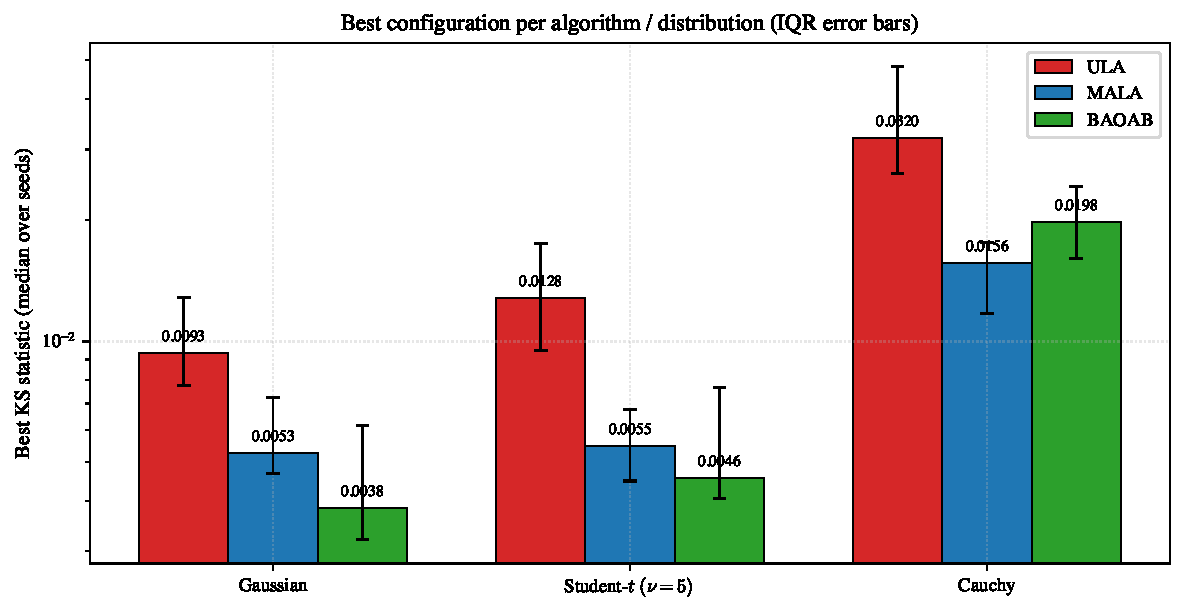
\includegraphics[width=0.85\textwidth]{../../experiments/figures/original_thesis/best_config_bars}
\caption{Καλύτερη στατιστική KS ανά αλγόριθμο σε κάθε κατανομή-στόχο, με
ράβδους σφάλματος IQR. \textbf{Χαμηλότερες τιμές είναι καλύτερες}. Ο BAOAB και ο MALA
είναι παρόμοιοι στη Γκαουσιανή και τη Student-$t$. Στην Cauchy, ο MALA
επιτυγχάνει τη χαμηλότερη KS, αλλά το χάσμα μεταξύ MALA και BAOAB είναι πολύ
μικρότερο από το χάσμα μεταξύ οποιουδήποτε εξ αυτών και του ULA.}
\label{fig:best-bars}
\end{figure}

Η κύρια κατάταξη που προκύπτει από τον Πίνακα~\ref{tab:best-configs} είναι:

\begin{itemize}
  \item Στη Γκαουσιανή και τη Student-$t$, ο BAOAB επιτυγχάνει τη χαμηλότερη διάμεσο KS ($0.0041$ και $0.0046$ αντίστοιχα), με τον MALA σε κοντινή δεύτερη θέση ($0.0056$ και $0.0055$). Η διαφορά μεταξύ BAOAB και MALA είναι αρκετά μικρή ώστε να εμπίπτει εντός της μεταβλητότητας μεταξύ εκτελέσεων.
  \item Στην Cauchy, ο MALA επιτυγχάνει τη χαμηλότερη διάμεσο KS ($0.0156$). Ο BAOAB καταλαμβάνει τη δεύτερη θέση ($0.0198$) και ο ULA την τρίτη με μεγάλη απόσταση ($0.0320$).
  \item Ο ULA είναι ο χειρότερος δειγματολήπτης σε κάθε κατανομή-στόχο. Η καλύτερη KS του είναι περίπου διπλάσια από εκείνες του MALA και του BAOAB στη Γκαουσιανή και τη Student-$t$, ενώ το χάσμα διευρύνεται περαιτέρω στην Cauchy.
\end{itemize}

Και οι δύο κύριες στρατηγικές διόρθωσης --- ο έλεγχος Metropolis στον MALA και ο
splitting ολοκληρωτής στον BAOAB --- παρέχουν ουσιαστικές βελτιώσεις έναντι της
απλής διακριτοποίησης Euler--Maruyama του ULA, ενώ η σχετική κατάταξη μεταξύ
MALA και BAOAB εξαρτάται από τη βαρύτητα ουράς της κατανομής-στόχου.

\subsection{Ετυμηγορία ανά Αλγόριθμο}

\paragraph{ULA --- μόνιμη μεροληψία σε κάθε κατανομή-στόχο.}
Ο ULA επιτυγχάνει τη βέλτιστη KS για τη Γκαουσιανή στο $\eta=0.05$, με διάμεσο
$0.0093$, περίπου διπλάσια από εκείνη του MALA ή του BAOAB. Η μεροληψία είναι
ορατή ακόμη και όταν η αλυσίδα αναμειγνύεται καλά: στο $\eta=0.05, d=1$ η
αυτοσυσχέτιση σε υστέρηση-100 είναι ουσιαστικά μηδέν για τη Γκαουσιανή, οπότε
η αλυσίδα εξερευνά το support --- απλώς εξερευνά ένα ελαφρώς \emph{λανθασμένο}
support. Αυτό δείχνει στην πράξη τη μόνιμη μεροληψία $\mathcal{O}(\eta)$ του ULA
που συζητείται στο Κεφάλαιο~\ref{chap:algorithms}.

Η μεροληψία επιδεινώνεται καθώς αυξάνεται η βαρύτητα ουράς. Για τη Student-$t$ η
βέλτιστη KS του ULA ανεβαίνει σε $0.0128$. Για την Cauchy ανεβαίνει περαιτέρω
σε $0.0320$. Η συμπεριφορά κάλυψης ουράς σε σταθερό βήμα $\eta=0.10$
τεκμηριώνεται στην Ενότητα~\ref{sec:tail-correlation} και αποτελεί τον κεντρικό
τρόπο αποτυχίας του ULA στη μελέτη αυτή.

\paragraph{MALA --- ο πιο αποδοτικός δειγματολήπτης σε ελαφριές και μέτριες ουρές.
Ο πιο ακριβής σε βαριές ουρές.}
Ο MALA επιτυγχάνει το υψηλότερο ESS στο σύνολο της μελέτης --- $36{,}047$
αποτελεσματικά δείγματα από $45{,}000$ για τη Γκαουσιανή στο $d=1$, που
αντιστοιχεί σε λόγο ESS ανά επανάληψη $0.80$, πλησίον της αναλογίας που
επιτυγχάνεται με πραγματικά ανεξάρτητα δείγματα. Τα ποσοστά αποδοχής βρίσκονται
στο εύρος $[0.78, 0.83]$ στις βέλτιστες διαμορφώσεις για τη Γκαουσιανή και τη
Student-$t$. Στην Cauchy το βέλτιστο μετατοπίζεται σε μεγαλύτερο βήμα ($\eta=4.0$)
με το ποσοστό αποδοχής να πέφτει στο $0.52$.

Το ποσοστό αποδοχής μειώνεται τόσο με τη διάσταση όσο και με τη βαρύτητα ουράς.
Στο $d=10$ για την Cauchy, η διάμεση αποδοχή στο $\eta=0.5$ είναι $0.78$, ενώ
στο $\eta=4.0$ είναι $0.49$. Αντιδιαισθητικά, για οποιοδήποτε κοινό βήμα ο
MALA αποδέχεται \emph{συχνότερα} για τη Student-$t$ παρά για τη Γκαουσιανή
(στο $\eta=1.0$, $d=1$: $0.82$ έναντι $0.78$): οι βαριές ουρές σημαίνουν ότι η
λογαριθμική πυκνότητα είναι πιο επίπεδη και ο λόγος Metropolis λιγότερο
κεντρωμένος, οπότε οι προτάσεις απορρίπτονται λιγότερο επιθετικά.
Το Σχήμα~\ref{fig:mala-accept} απεικονίζει την πλήρη συμπεριφορά αποδοχής ως
συνάρτηση του $\eta$ και του $d$, με σκίαση της ασυμπτωτικής ζώνης αναφοράς
$[0.234, 0.574]$, της οποίας το άνω άκρο $0.574$ είναι το βέλτιστο ποσοστό
αποδοχής για τον MALA ενώ το κάτω άκρο $0.234$ αντιστοιχεί στον Random-Walk
Metropolis \citep{roberts1998optimal}. Και τα δύο όρια είναι υπερβολικά χαμηλά
για $d\le 10$ και τα εμπειρικά βέλτιστά μας βρίσκονται πάνω από αυτήν.

\begin{figure}[ht]
\centering
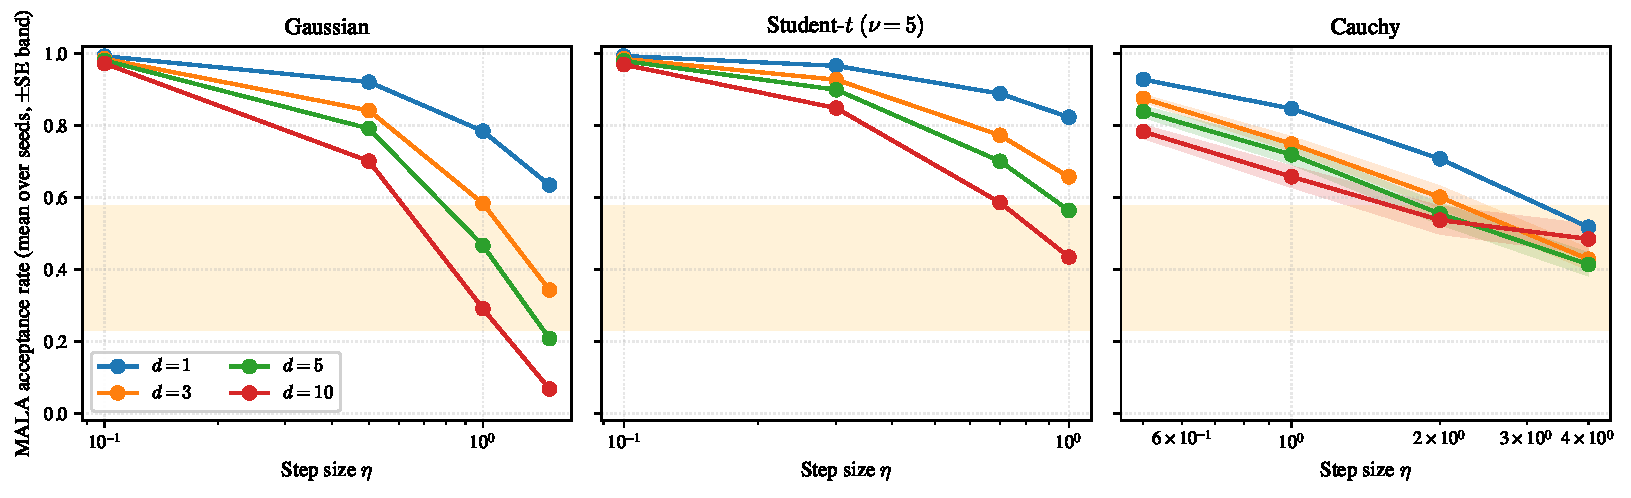
\includegraphics[width=\textwidth]{../../experiments/figures/original_thesis/mala_acceptance}
\caption{Ποσοστό αποδοχής του MALA ως συνάρτηση του βήματος και της διάστασης,
στις τρεις κατανομές-στόχους. Κάθε γραμμή είναι ο μέσος μεταξύ $20$ εκτελέσεων με
ζώνη σκίασης $\pm$ τυπικό σφάλμα. Οι γραμμές χρωματίζονται ανά διάσταση. Η
πορτοκαλί ζώνη σηματοδοτεί την ασυμπτωτική περιοχή αναφοράς $[0.234, 0.574]$
(άνω άκρο $0.574$ = βέλτιστο MALA, κάτω άκρο $0.234$ = βέλτιστο Random-Walk
Metropolis).}
\label{fig:mala-accept}
\end{figure}

\paragraph{BAOAB --- H μικρότερη απόκλιση σε ελαφριές ουρές στο $d=1$,
με τις μικρότερες μεροληψίες ροπών.}
Ο BAOAB επιτυγχάνει τη χαμηλότερη διάμεσο KS στο $d=1$ για τη Γκαουσιανή
($0.0041$) και τη Student-$t$ ($0.0046$), υπερτερώντας οριακά του MALA και στις
δύο περιπτώσεις. Το πλεονέκτημα έναντι του MALA είναι της τάξης $25$--$50\%$
στο KS στατιστικό. Το ESS στο $d=1$ είναι περίπου το μισό εκείνου του MALA για τη Γκαουσιανή ($20{,}500$ έναντι $36{,}000$). Ο BAOAB δεν έχει απορριπτόμενες προτάσεις αλλά απαιτεί δύο
αξιολογήσεις κλίσης ανά βήμα αντί για μία συν μία αξιολόγηση λογαριθμικής
πυκνότητας, οπότε η σύγκριση ως προς χρόνο εκτέλεσης είναι πιο κοντινή από
ό,τι υποδηλώνει η διαφορά ESS.

Επιπλέον, ο BAOAB παράγει τις μικρότερες μεροληψίες ροπών από τους τρεις
αλγορίθμους στη Γκαουσιανή και τη Student-$t$ κατανομή-στόχο. Στο $d=1$ για
τη Γκαουσιανή, η απόλυτη μεροληψία του εκτιμητή μέσου είναι $0.001$ και του
εκτιμητή διακύμανσης $0.0003$ --- περίπου πέντε φορές μικρότερες από τις
μεροληψίες του MALA για τον ίδιο στόχο. Το σφάλμα διακριτοποίησης του BAOAB
ολοκληρωτή είναι ανώτερης τάξης από εκείνο του ULA, κάτι που εκδηλώνεται σε
αυτού του είδους τη λεπτομερή σύγκριση ακρίβειας.

Η δομικά σημαντική ιδιότητα του BAOAB --- ότι η KS του για τη Γκαουσιανή
κατανομή-στόχο παραμένει περίπου σταθερή καθώς αυξάνεται η διάσταση ---
αναλύεται στην Ενότητα~\ref{sec:dim-scaling}, όπου ο πίνακας κλιμάκωσης
διάστασης καθιστά ρητή τη σύγκριση με τον MALA.

\subsection{Ευαισθησία στην Παράμετρο Τριβής $\gamma$ του BAOAB}
\label{sec:gamma-sensitivity}

Ο BAOAB ολοκληρωτής εξαρτάται από μια παράμετρο τριβής $\gamma$ που ελέγχει
πόσο γρήγορα αποσβένεται η ορμή. Μικρό $\gamma$ επιτρέπει στην ορμή να
συσσωρεύεται μεταξύ βημάτων. Μεγάλο $\gamma$
αναγκάζει την ορμή να αποκαθίσταται γρήγορα (καθεστώς διαχυτικής κίνησης, εμφανίζοντας παρόμοια συμπεριφορά με τον ULA).

Λαμβάνοντας μέσο όρο επί των διαμορφώσεων $(\eta, d)$, η μέση KS βελτιώνεται
μονότονα για μικρό $\gamma$ σε κάθε κατανομή-στόχο:

\begin{table}[ht]
\centering
\small
\begin{tabular}{lcccc}
\toprule
                & $\gamma = 0.5$ & $\gamma = 1.0$ & $\gamma = 2.0$ & $\gamma = 5.0$ \\
\midrule
Γκαουσιανή KS     & $0.0064$ & $0.0072$ & $0.0084$ & $0.0110$ \\
Student-$t$ KS  & $0.0081$ & $0.0088$ & $0.0101$ & $0.0134$ \\
Cauchy KS       & $0.0421$ & $0.0498$ & $0.0596$ & $0.0830$ \\
\bottomrule
\end{tabular}
\caption{Μέση KS επί των διαμορφώσεων $(\eta, d)$, ανά τιμή τριβής $\gamma$.
Σε κάθε κατανομή-στόχο η διάμεση KS βελτιώνεται ομαλά καθώς το $\gamma$
μειώνεται.}
\label{tab:gamma-mean}
\end{table}

Ο κανόνας «μικρό $\gamma$ είναι καλύτερο» ισχύει στο επίπεδο της διαμέσου KS
κατά μέσο όρο ως προς τις υπερπαραμέτρους. Σε επίπεδο μεμονωμένων βέλτιστων
διαμορφώσεων η εικόνα είναι λιγότερο ξεκάθαρη: για τον BAOAB στη Γκαουσιανή
στο $d=1, \eta=1.0$, και οι τέσσερις τιμές $\gamma$ παράγουν στατιστικώς
αδιάκριτες διαμέσους KS (οι τέσσερις διάμεσοι καλύπτουν μόνο το διάστημα
$0.0038$--$0.0041$, καλά εντός του IQR της καθεμίας). Αυτό που τις διαφοροποιεί
σε αυτή τη βέλτιστη διαμόρφωση είναι το ESS: το $\gamma=0.5$ παρέχει $20{,}498$
αποτελεσματικά δείγματα έναντι $11{,}865$ στο $\gamma=5.0$, βελτίωση $70\%$.
Με άλλα λόγια, η χαμηλή τριβή είναι η ασφαλής επιλογή όταν δεν είναι εφικτή
ακριβής ρύθμιση εκ των προτέρων. Το Σχήμα~\ref{fig:baoab-gamma} απεικονίζει
αυτήν την τάση.

\begin{figure}[ht]
\centering
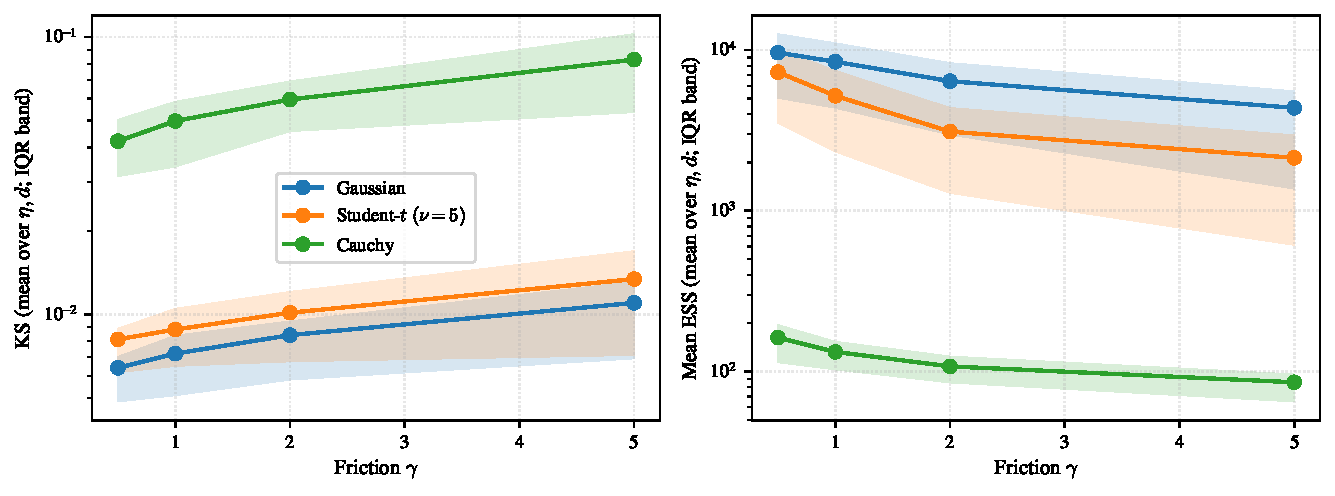
\includegraphics[width=\textwidth]{../../experiments/figures/original_thesis/baoab_gamma_sensitivity}
\caption{Ευαισθησία του BAOAB στην παράμετρο τριβής $\gamma$ στις τρεις
κατανομές-στόχους, με ζώνες σφάλματος IQR. Τόσο το πλαίσιο KS (αριστερά) όσο
και το πλαίσιο ESS (δεξιά) ευνοούν μικρό $\gamma$ κατά μέσο όρο επί του
πλέγματος υπερπαραμέτρων.}
\label{fig:baoab-gamma}
\end{figure}

Αυτό το εμπειρικό μοτίβο αντιφάσκει με μια κοινή εγχειριδιακή διαίσθηση ότι
οι βαρύτερες ουρές ωφελούνται από \emph{περισσότερη} τριβή \citep{leimkuhler2015molecular} (επειδή η αλυσίδα
χρειάζεται να αποσβεστεί ενάντια στις μακρές εκδρομές). Τα εμπειρικά δεδομένα
είναι αναμφίβολα: και στις τρεις κατανομές-στόχους, η χαμηλή τριβή κερδίζει
κατά μέσο όρο, τόσο στην KS όσο και στο ESS.

\subsection{Κλιμάκωση ως προς τη Διάσταση}
\label{sec:dim-scaling}

Επεκτείνουμε το πλέγμα από $d \in \{1, 3, 5, 10\}$ σε
$d \in \{20, 50, 100\}$ και εξετάζουμε εκ νέου τη μέση KS ανά αλγόριθμο σε
κάθε διάσταση. Το κεντρικό αποτέλεσμα, ορατό στον
Πίνακα~\ref{tab:dim-scaling-numbers} παρακάτω, είναι ότι \emph{η KS του BAOAB
για τη Γκαουσιανή κατανομή-στόχο είναι ουσιαστικά σταθερή σε ολόκληρο το
εξεταζόμενο εύρος διαστάσεων}. Η τιμή του KS στις 100 διαστάσεις (0.006) διαφέρει ελάχιστα από την αντίστοιχη της μίας διάστασης (0.007). Σε σύγκριση, η μέση KS του MALA για τη Γκαουσιανή αυξάνεται κατά παράγοντα $15$ στο ίδιο εύρος (από
$0.007$ σε $0.109$). Αυτό αποτελεί το ισχυρότερο εμπειρικό τεκμήριο υπέρ του underdamped σχήματος όσον αφορά τη συμπεριφορά του σε υψηλές
διαστάσεις για λογαριθμικά-κυρτές κατανομές-στόχους.

Το Σχήμα~\ref{fig:dim-scaling} απεικονίζει τη μέση KS ως συνάρτηση της
διάστασης για $d \in \{1, 3, 5, 10, 20, 50, 100\}$, κατά μέσο όρο επί των
διαμορφώσεων $(\eta, \gamma)$. Ο Πίνακας~\ref{tab:dim-scaling-numbers} παρέχει
τις υποκείμενες αριθμητικές τιμές.

\begin{table}[ht]
\centering
\small
\begin{tabular}{llccccccc}
\toprule
Αλγ. & Κατανομή & $d{=}1$ & $d{=}3$ & $d{=}5$ & $d{=}10$ & $d{=}20$ & $d{=}50$ & $d{=}100$ \\
\midrule
ULA   & Γκαουσιανή    & $0.015$ & $0.018$ & $0.020$ & $0.020$ & $0.021$ & $0.021$ & $0.020$ \\
ULA   & Student-$t$ & $0.026$ & $0.031$ & $0.035$ & $0.045$ & $0.034$ & $0.045$ & $0.064$ \\
ULA   & Cauchy      & $0.042$ & $0.060$ & $0.065$ & $0.096$ & $0.258$ & $0.599$ & $0.640$ \\
MALA  & Γκαουσιανή    & $0.007$ & $0.008$ & $0.010$ & $0.015$ & $0.012$ & $0.040$ & $0.109$ \\
MALA  & Student-$t$ & $0.008$ & $0.008$ & $0.010$ & $0.012$ & $0.016$ & $0.031$ & $0.031$ \\
MALA  & Cauchy      & $0.020$ & $0.029$ & $0.049$ & $0.074$ & $0.080$ & $0.348$ & $0.593$ \\
BAOAB & Γκαουσιανή    & $0.007$ & $0.008$ & $0.009$ & $0.009$ & $0.006$ & $0.006$ & $0.006$ \\
BAOAB & Student-$t$ & $0.008$ & $0.010$ & $0.010$ & $0.011$ & $0.012$ & $0.012$ & $0.013$ \\
BAOAB & Cauchy      & $0.042$ & $0.056$ & $0.061$ & $0.075$ & $0.125$ & $0.497$ & $0.566$ \\
\bottomrule
\end{tabular}
\caption{Μέσος της διαμέσου KS επί των διαμορφώσεων $(\eta, \gamma)$, ανά ζεύγος
(αλγόριθμος, κατανομή, διάσταση). Οι κατανομές-στόχοι Γκαουσιανή και Student-$t$
υποβαθμίζονται αργά με τη διάσταση και για τους τρεις αλγορίθμους. Η κατανομή
Cauchy υποβαθμίζεται σοβαρά και για τους τρεις, ιδίως πέραν του $d = 10$.
Σημειώστε τη στήλη Γκαουσιανής του BAOAB: η KS παραμένει στο $\approx 0.006$
ως και το $d = 100$.}
\label{tab:dim-scaling-numbers}
\end{table}

Τρία μοτίβα είναι ορατά:

\begin{itemize}
\item \textbf{Για τη Γκαουσιανή κατανομή-στόχο}, και οι τρεις αλγόριθμοι
      παραμένουν σταθεροί έως το $d = 100$, με αμετάβλητη σειρά αξίας. Η KS
      του BAOAB είναι ουσιαστικά σταθερή στο $\approx 0.006$ σε ολόκληρο το
      εξεταζόμενο εύρος διαστάσεων --- η ανθεκτικότητα ως προς τη διάσταση του
      underdamped σχήματος είναι εντυπωσιακή. Ο MALA υποβαθμίζεται πιο εμφανώς
      σε υψηλό $d$ (από $0.007$ στο $d=1$ σε $0.109$ στο $d=100$), καθώς το
      ποσοστό αποδοχής του κινείται προς το ασυμπτωτικό καθεστώς
      Roberts--Rosenthal που συζητείται στην Ενότητα~\ref{sec:grid-study}.
\item \textbf{Για τη Student-$t$ κατανομή-στόχο}, και οι τρεις αλγόριθμοι
      παραμένουν εύλογοι σε ολόκληρο το εύρος. Η μεροληψία του ULA αυξάνεται με
      τη διάσταση ($0.026 \to 0.064$). Η KS του MALA αυξάνεται παρόμοια. Ο BAOAB
      παρακολουθεί στενά τον MALA καθ' όλη τη διάρκεια.
\item \textbf{Για τη Cauchy κατανομή-στόχο}, και οι τρεις αλγόριθμοι
      υποβαθμίζονται σοβαρά πέραν του $d = 10$, και στο $d = 100$ οι μέσες
      τιμές KS και των τριών είναι πάνω από $0.5$ --- λειτουργικά, κανένας από
      αυτούς δεν δειγματίζει την κατανομή-στόχο στο $d = 100$. Η πτώση είναι
      πιο απότομη μεταξύ $d = 10$ και $d = 50$. Στο $d = 100$ οι τρεις
      αλγόριθμοι είναι ουσιαστικά ισόπαλοι σε επίπεδο αποτυχίας. Αυτή είναι η
      σημαντικότερη εμπειρική παρατήρηση σχετικά με τη δειγματοληψία βαριών
      ουρών σε αυτή την εργασία: η δυσκολία δεν κλιμακώνεται ήπια με τη
      διάσταση αλλά αλλάζει το καθεστώς κάπου στο $20 \le d \le 50$.
\end{itemize}

Αξίζει επίσης να σημειωθεί ότι η αναλογία ESS του BAOAB για τη Γκαουσιανή
παραμένει σταθερή ανεξάρτητα από τη διάσταση. Το μέσο ESS μεταξύ διαμορφώσεων στο $d=1$ είναι
περίπου $9{,}600$ και στο $d=10$ περίπου $4{,}500$. Στο $d = 100$ παραμένει
πάνω από $1{,}000$, μια αργή λογαριθμική πτώση αντί της πτώσης κατά παράγοντα
πέντε ανά δεκάδα που εκδηλώνει ο MALA στο ίδιο εύρος. Αυτό δείχνει στην πράξη γιατί τα underdamped σχήματα έχουν προσελκύσει τόσο
ενδιαφέρον στη σύγχρονη βιβλιογραφία για kinetic δειγματολήπτες Langevin
\citep{cheng2018underdamped, leimkuhler2015molecular, neal2011mcmc}, και
ισχύει έως τις μεγαλύτερες διαστάσεις που δοκιμάσαμε.

\begin{figure}[ht]
\centering
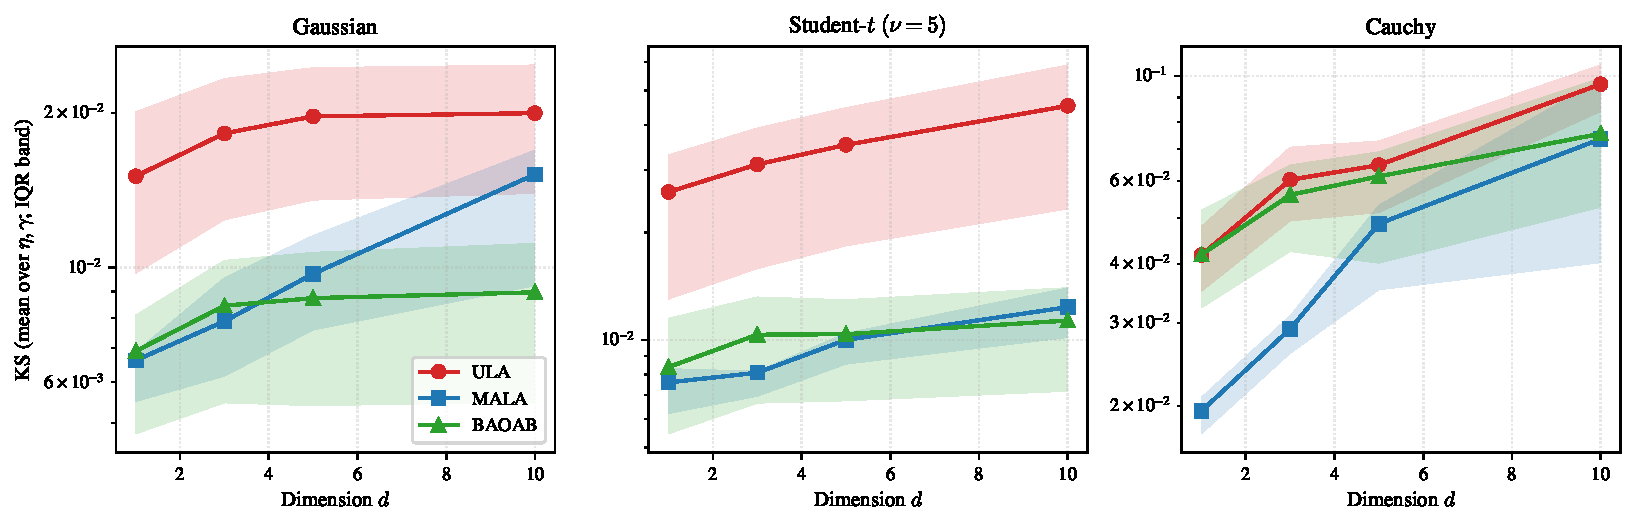
\includegraphics[width=\textwidth]{../../experiments/figures/original_thesis/dimension_scaling_ks}
\caption{KS ως συνάρτηση της διάστασης, κατά μέσο όρο επί του
πλέγματος $(\eta, \gamma)$ για κάθε αλγόριθμο. Η σκιασμένη ζώνη δείχνει το
διατεταρτημοριακό εύρος των διαμέσων ανά διαμόρφωση. Και οι δύο άξονες είναι
σε λογαριθμική κλίμακα.}
\label{fig:dim-scaling}
\end{figure}

\subsection{Κόστος Χρόνου Εκτέλεσης}
\label{sec:exec-time}

Το κόστος ανά επανάληψη κάθε δειγματολήπτη διαφέρει: ο ULA εκτελεί μία
αξιολόγηση κλίσης ανά βήμα. Ο MALA εκτελεί μία αξιολόγηση κλίσης και μία
αξιολόγηση λογαριθμικής πυκνότητας, συν έναν έλεγχο αποδοχής/απόρριψης. Ο
BAOAB εκτελεί δύο αξιολογήσεις κλίσης ανά βήμα στις ενημερώσεις μισής δύναμης
και δεν έχει έλεγχο αποδοχής/απόρριψης. Αν αυτές οι διαφορές ανά βήμα
μεταφράζονται σε χρήσιμες διαφορές χρόνου εκτέλεσης εξαρτάται από την
υλοποίηση, το κόστος κλίσης της κατανομής-στόχου και τη διάσταση. Ο
Πίνακας~\ref{tab:runtime-cost} παρέχει τους εμπειρικούς αριθμούς στο $d=1$ για
κάθε κατανομή-στόχο, μετρημένους στην υλοποίησή μας που χρησιμοποιεί τα πακέτα NumPy/SciPy. Το ESS ανά δευτερόλεπτο συνδυάζει χρόνο εκτέλεσης και αποτελεσματικό
μέγεθος δείγματος και αποτελεί την τυπική μετρική αποδοτικότητας προσαρμοσμένης
ως προς το κόστος για MCMC.

\begin{table}[H]
\centering
\small
\begin{tabular}{llrrr}
\toprule
Αλγόριθμος & Κατανομή-στόχος & Χρόνος εκτέλεσης (s) & ESS & ESS / sec \\
\midrule
ULA   & Γκαουσιανή    & $0.14$ & $1{,}205$  & $\phantom{0}8{,}600$ \\
ULA   & Student-$t$ & $0.27$ & $\phantom{1}608$    & $\phantom{0}2{,}250$ \\
ULA   & Cauchy      & $0.25$ & $\phantom{1}124$    & $\phantom{0}\phantom{0}495$ \\
MALA  & Γκαουσιανή    & $0.60$ & $16{,}900$ & $28{,}000$ \\
MALA  & Student-$t$ & $1.10$ & $12{,}800$ & $11{,}550$ \\
MALA  & Cauchy      & $1.01$ & $\phantom{1}576$    & $\phantom{0}\phantom{0}563$ \\
BAOAB & Γκαουσιανή    & $0.35$ & $14{,}800$ & $41{,}900$ \\
BAOAB & Student-$t$ & $0.64$ & $\phantom{1}6{,}800$  & $10{,}600$ \\
BAOAB & Cauchy      & $0.58$ & $\phantom{1}262$    & $\phantom{0}\phantom{0}453$ \\
\bottomrule
\end{tabular}
\caption{Χρόνος εκτέλεσης ανά αλυσίδα και αποδοτικότητα στο $d=1$, βέλτιστη
διαμόρφωση ανά ζεύγος (αλγόριθμος, κατανομή-στόχος). Ο χρόνος εκτέλεσης είναι
ανά $5\!\times\!10^4$ επαναλήψεις, μέσος μεταξύ $20$ εκτελέσεων. Το κόστος ανά
επανάληψη του ULA είναι το χαμηλότερο αλλά το χαμηλό ESS του δίνει το χειρότερο
ESS ανά δευτερόλεπτο. Ο BAOAB και ο MALA βρίσκονται εντός παράγοντα $1.5$ στο
ESS ανά δευτερόλεπτο για τη Γκαουσιανή και τη Student-$t$ στο $d=1$. Στην Cauchy
και οι τρεις αλγόριθμοι περιορίζονται από το χαμηλό τους ESS παρά από το κόστος
ανά επανάληψη.}
\label{tab:runtime-cost}
\end{table}

Η εικόνα στο $d=1$ είναι ότι \textbf{ο MALA και ο BAOAB είναι συγκρίσιμοι σε
αποδοτικότητα χρόνου εκτέλεσης για τη Γκαουσιανή και τη Student-$t$
κατανομή-στόχο}, με τον BAOAB περίπου $50\%$ μπροστά για τη Γκαουσιανή και τον
MALA περίπου $10\%$ μπροστά για τη Student-$t$. Το χάσμα κλείνει περαιτέρω στην
Cauchy, όπου και οι τρεις αλγόριθμοι παράγουν τόσο λίγο ESS ανά αλυσίδα ώστε
ο χρόνος-ρολογιού ανά ESS να κυριαρχείται από τη δυσκολία της κατανομής-στόχου
παρά από την επιβάρυνση οποιουδήποτε αλγορίθμου.

Η εικόνα αλλάζει δραματικά καθώς η διάσταση αυξάνεται.
Το Σχήμα~\ref{fig:ess-per-sec} απεικονίζει το ESS ανά δευτερόλεπτο ως συνάρτηση
της διάστασης στη βέλτιστη διαμόρφωση ανά αλγόριθμο για τη Γκαουσιανή
κατανομή-στόχο.

\begin{figure}[H]
\centering
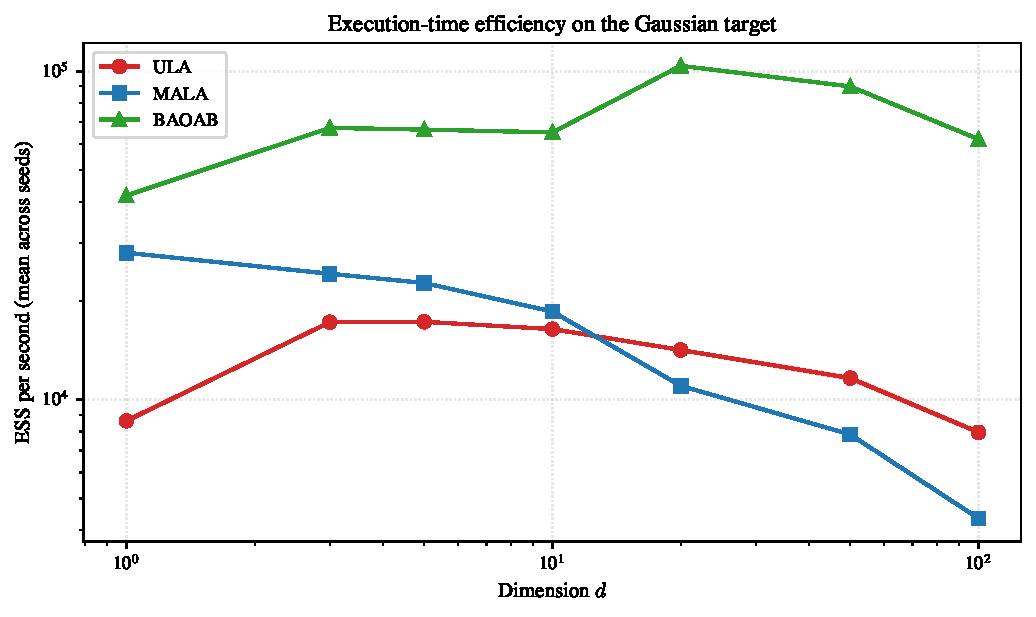
\includegraphics[width=0.85\textwidth]{../../experiments/figures/original_thesis/ess_per_sec_gaussian}
\caption{ESS ανά δευτερόλεπτο ως συνάρτηση της διάστασης στη βέλτιστη διαμόρφωση
ανά αλγόριθμο για τη Γκαουσιανή κατανομή-στόχο. Και οι δύο άξονες είναι
λογαριθμικοί. Η αποδοτικότητα του BAOAB αυξάνεται με τη διάσταση έως
$d\approx 20$ και παραμένει μια τάξη μεγέθους πάνω από τον MALA στο $d=100$.}
\label{fig:ess-per-sec}
\end{figure}

Δύο χαρακτηριστικά του Σχήματος~\ref{fig:ess-per-sec} αξίζουν προσοχής.
Πρώτον, το ESS ανά δευτερόλεπτο του BAOAB για τη Γκαουσιανή \emph{αυξάνεται} με τη διάσταση, από $42{,}000$ στο $d=1$ σε κορύφωση
$104{,}000$ στο $d=20$, πριν μειωθεί αργά σε $62{,}000$ στο $d=100$. Αυτό
αντικατοπτρίζει δύο παράγοντες: η KS του BAOAB παραμένει περίπου σταθερή καθώς
αυξάνεται το $d$ (Ενότητα~\ref{sec:dim-scaling}), και το κόστος ανά επανάληψη
αυξάνεται μόνο ελαφρά με το $d$ στην υλοποίησή μας NumPy επειδή η αλυσίδα
επεξεργάζεται όλες τις συντεταγμένες σε διανυσματοποιημένες πράξεις πίνακα.
Δεύτερον, \textbf{το ESS ανά δευτερόλεπτο του MALA πέφτει απότομα με τη
διάσταση}, από $28{,}000$ στο $d=1$ σε $4{,}400$ στο $d=100$. Στο $d=10$ ο
BAOAB είναι περίπου $3.5\times$ πιο αποδοτικός από τον MALA ανά δευτερόλεπτο.
Στο $d=100$, $14\times$ πιο αποδοτικός.

Η ανθεκτικότητα του BAOAB ως προς τη διάσταση οδηγεί συνεπώς σε πολύ καλύτερη
απόδοση σε σχέση με το υπολογιστικό κόστος από ό,τι υποδηλώνει μόνη της η
σύγκριση ESS ανά επανάληψη. Η αλγοριθμική σύσταση
που προκύπτει είναι απλή: \emph{για δειγματοληψία μέτριας έως υψηλής διάστασης
σε λογαριθμικά-κυρτές κατανομές-στόχους, ο BAOAB παρέχει ουσιαστικά
περισσότερα αποτελεσματικά δείγματα ανά δευτερόλεπτο από τον MALA στην
υλοποίησή μας.}

\section{Βαρύτητα Ουράς και Μεροληψία}
\label{sec:tail-correlation}

Το κεντρικό ερώτημα της εργασίας είναι πώς οι τρεις δειγματολήπτες
ανταποκρίνονται στην αυξανόμενη βαρύτητα ουράς. Απομονώνουμε την επίδραση
καθηλώνοντας $d=1$ και $\eta=0.10$ για τον ULA --- ένα βήμα παρόν στο πλέγμα
ULA και για τις τρεις κατανομές-στόχους --- και συγκρίνουμε τι κάνει η αλυσίδα
στις τρεις κατανομές. Το Σχήμα~\ref{fig:ula-bias} δείχνει το αποτέλεσμα, και ο
Πίνακας~\ref{tab:ula-tails} συλλέγει τους υποκείμενους αριθμούς.

\begin{table}[ht]
\centering
\small
\begin{tabular}{lccccc}
\toprule
Κατανομή     & διάμεση KS              & q-MAE q=0.025 & q-MAE q=0.975 & κάλ. ουράς q=0.01 & κάλ. ουράς q=0.99 \\
\midrule
Γκαουσιανή         & $0.0099$ ($0.0080, 0.0140$)  & $0.052$ & $0.050$ & $1.17$ & $1.17$ \\
Student-$t$      & $0.0131$ ($0.0103, 0.0176$)  & $0.048$ & $0.102$ & $0.98$ & $1.02$ \\
Cauchy           & $0.0359$ ($0.0292, 0.0549$)  & $6.54$  & $5.15$  & $0.00$ & $0.00$ \\
\bottomrule
\end{tabular}
\caption{Διαγνωστικά ULA στο $\eta=0.10$, $d=1$, για τις τρεις κατανομές-στόχους.
Διάμεσος μεταξύ $20$ εκτελέσεων. IQR σε παρένθεση για τη στήλη KS. Οι αναλογίες
κάλυψης ουράς στις δύο τελευταίες στήλες θα έπρεπε να είναι $1.0$ σε έναν
ιδανικά συμπεριφερόμενο δειγματολήπτη.}
\label{tab:ula-tails}
\end{table}

\begin{figure}[ht]
\centering
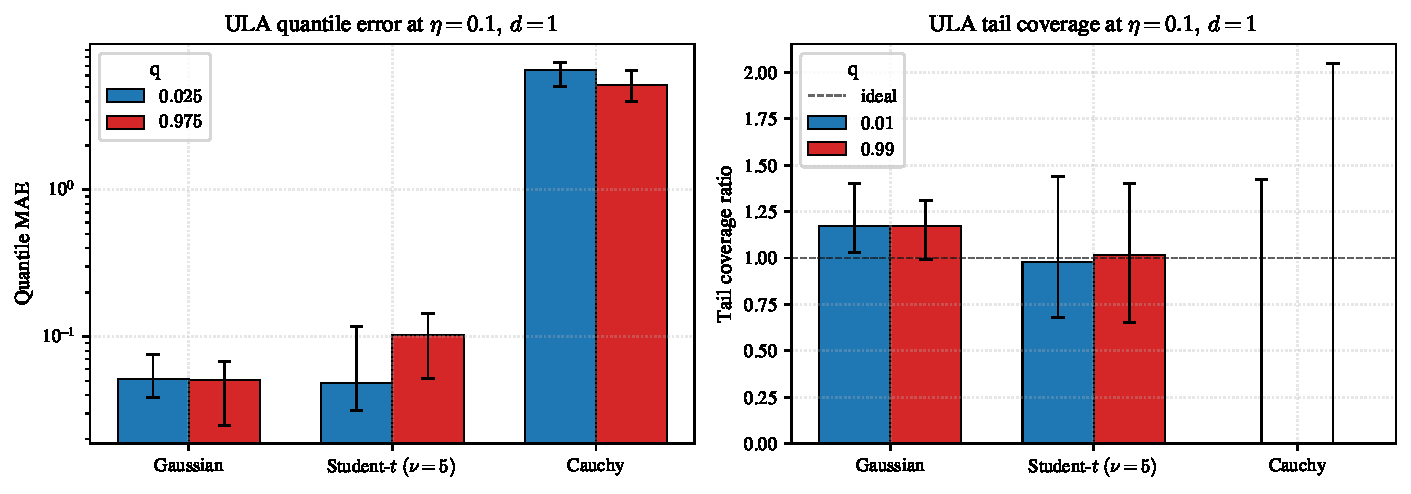
\includegraphics[width=\textwidth]{../../experiments/figures/original_thesis/ula_bias_inversion}
\caption{ULA στο ίδιο βήμα για τις τρεις κατανομές-στόχους. Αριστερά: σφάλμα
στα εμπειρικά ποσοστημόρια $2.5\%$ και $97.5\%$, με ράβδους σφάλματος IQR σε
λογαριθμική κλίμακα. Δεξιά: αναλογίες κάλυψης ουράς στο $1\%$ και $99\%$.
Η οριζόντια γραμμή δείχνει την ιδανική τιμή $1.0$.}
\label{fig:ula-bias}
\end{figure}

Διακρίνονται τρία διακριτά καθεστώτα αποτυχίας:

\begin{enumerate}
  \item \textbf{Γκαουσιανή (ελαφριές ουρές):} ο ULA \emph{υπερ-καλύπτει} τις
        ουρές κατά περίπου $17\%$ (αναλογία κάλυψης ουράς $1.17$). Η αλυσίδα
        τοποθετεί ελαφρώς περισσότερη μάζα πέραν του θεωρητικού ποσοστημορίου
        $99\%$ από ό,τι έπρεπε. Τα εμπειρικά ακραία ποσοστημόρια είναι ήπια
        υπερβολικά ακραία. Τα σφάλματα ποσοστημορίου στα επίπεδα $2.5\%/97.5\%$
        είναι της τάξης $0.05$ --- μικρά σε απόλυτους όρους αλλά ορατά.
  \item \textbf{Student-$t$ (μέτριες ουρές):} η υπερ-κάλυψη της Γκαουσιανής
        εξαφανίζεται και οι αναλογίες κάλυψης ουράς είναι ουσιαστικά μοναδιαίες.
        Το σφάλμα ποσοστημορίου στο άνω άκρο διπλασιάζεται ($0.05 \to 0.10$) ---
        η αλυσίδα έχει περίπου το σωστό σχήμα αλλά τα εμπειρικά ακραία
        ποσοστημόρια είναι πιο θορυβώδη.
  \item \textbf{Cauchy (βαριές ουρές):} ο τρόπος μεροληψίας \emph{αντιστρέφεται}.
        Αντί να υπερ-καλύπτει τις ουρές, η αλυσίδα αποτυγχάνει να τις φτάσει. Η αναλογία κάλυψης ουράς στο $q=0.01$ και $q=0.99$ καταρρέει
        σε μηδέν σε κάθε μία από τις $20$ εκτελέσεις. Το σφάλμα ποσοστημορίου
        στο επίπεδο $97.5\%$ εκτοξεύεται από $0.05$ (Γκαουσιανή) σε $0.10$
        (Student-$t$) σε $5.15$ (Cauchy), μία εκατονταπλάσια αύξηση.
\end{enumerate}

Ο μηχανισμός είναι γεωμετρικός. Το βήμα πρότασης του ULA είναι
$-\eta \nabla U(X) + \sqrt{2\eta}\,\xi$. Για τη Γκαουσιανή, $\nabla U(x) = x$,
οπότε η ντετερμινιστική ολίσθηση πάντοτε επαναφέρει την αλυσίδα προς την αρχή
με δύναμη ανάλογη του $\|x\|$. Για την Cauchy, η κλίση είναι
$\nabla U(x) = (d+1) x / (1+\|x\|^2)$, η οποία τείνει \emph{στο μηδέν} καθώς
$\|x\|\to\infty$. Μόλις μια αλυσίδα Cauchy βρεθεί μακριά από την αρχή, δεν
υπάρχει ντετερμινιστική επαναφορική δύναμη, και ο μόνος μηχανισμός για να
παραμείνει στην ουρά ή να την αφήσει είναι ο όρος θορύβου, που έχει αναμενόμενο
μέγεθος $\sqrt{2\eta} \approx 0.45$ --- πολύ μικρότερο από το θεωρητικό
ποσοστημόριο $99\%$ της Cauchy στο $\pm 31.8$. Η αλυσίδα αδυνατεί να πραγματοποιήσει άλμα από την αρχή
στο $\pm 30$ σε πεπερασμένο χρόνο, ούτε, έχοντας φτάσει σε τέτοια περιοχή,
να επιστρέψει από αυτήν αποδοτικά.

Ο MALA αντισταθμίζει εν μέρει επιτρέποντας μεγαλύτερα βήματα (το βέλτιστο
$\eta$ για τον MALA στην Cauchy είναι $4.0$, οκτώ φορές μεγαλύτερο από εκείνο
του ULA), αλλά το ποσοστό αποδοχής Metropolis μειώνεται αντίστοιχα. Ο BAOAB
παρακάμπτει το πρόβλημα διαφορετικά --- η ενημέρωση Ornstein--Uhlenbeck στη μεταβλητή ταχύτητας επιτρέπει στην αλυσίδα
να κινείται προς μακρινές περιοχές με τη βοήθεια της ορμής, χωρίς να χρειάζεται
μια μεμονωμένη μεγάλη πρόταση.
Τεκμηριώνουμε τις συνέπειες στη μελέτη σύγκλισης
(Ενότητα~\ref{sec:convergence-study}) και στις μελέτες περίπτωσης που ακολουθούν.

\subsection{Εξάρτηση από τη Διάσταση των Ευρημάτων Ουράς}
\label{sec:dim-dependence-tails}

Το κεντρικό εύρημα αυτής της υποενότητας είναι μια \emph{αλλαγή καθεστώτος}
στη δειγματοληψία Cauchy μεταξύ $d=10$ και $d=50$. Κάτω από $d=10$ και οι τρεις
αλγόριθμοι διαχειρίζονται την Cauchy με μεταβλητό βαθμό επιτυχίας (μέση KS
βέλτιστης διαμόρφωσης στο $[0.02, 0.10]$). Στο $d=100$ και οι τρεις
αποτυγχάνουν λειτουργικά, με μέση KS πάνω από $0.5$ για κάθε αλγόριθμο. Η
κατάρρευση δεν είναι ομαλή υποβάθμιση: μεταξύ $d=10$ και $d=50$ η μέση KS
αυξάνεται κατά παράγοντα πέντε για κάθε αλγόριθμο, και πέραν του $d=50$ οι
διαφορές μεταξύ αλγορίθμων εξαφανίζονται. Πρόκειται για γεωμετρική ιδιότητα των
κατανομών βαριάς ουράς σε υψηλή διάσταση --- το τυπικό σύνολο μιας Cauchy στο
$\mathbb{R}^d$ μετακινείται προς τα έξω με $d$ ταχύτερα από ό,τι μπορεί να
ακολουθήσει οποιοσδήποτε δειγματολήπτης βασισμένος σε κλίση --- και δεν είναι πρόβλημα κάποιου συγκεκριμένου αλγορίθμου, αλλά
γεωμετρία των βαριών ουρών σε υψηλή διάσταση.

Η ποιοτική συμπεριφορά που μόλις περιγράφηκε --- πώς ο ULA αντιστρέφει την
μεροληψία, ο MALA αντισταθμίζει μεγεθύνοντας το βήμα, και ο BAOAB εκμεταλλεύεται
την ορμή --- είναι γεωμετρικά αναπόφευκτη σε κάθε διάσταση. Το εμπειρικό ερώτημα είναι πόσο
γρήγορα η δυσκολία αυξάνεται με $d$. Το Σχήμα~\ref{fig:cauchy-dim} απεικονίζει
τρία διαγνωστικά Cauchy --- την προσαρμογή κορμού (KS), το σφάλμα ακραίου
ποσοστημορίου (q-MAE στο $q=0.975$) και την αναλογία κάλυψης άνω ουράς --- ως
συνάρτηση της διάστασης για τη βέλτιστη διαμόρφωση κάθε αλγορίθμου σε εκείνη
τη διάσταση.

\begin{figure}[ht]
\centering
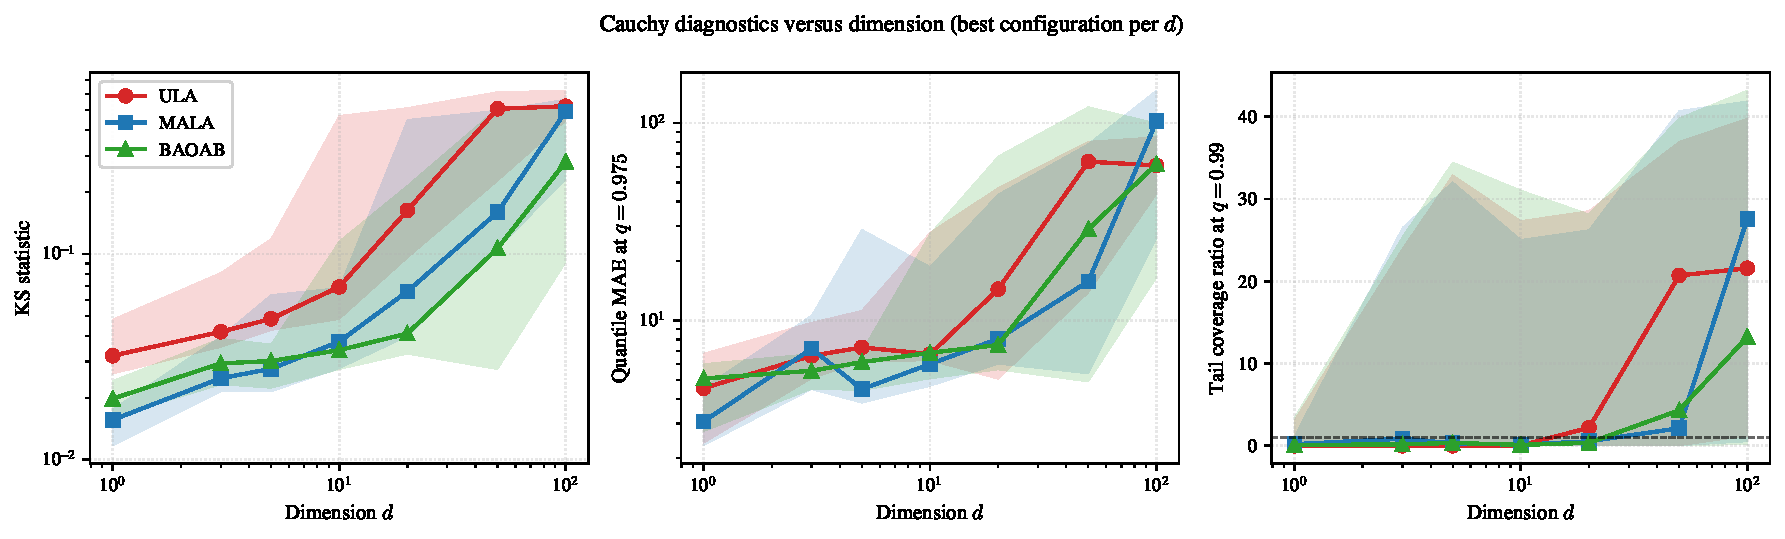
\includegraphics[width=\textwidth]{../../experiments/figures/original_thesis/cauchy_dimension_scaling}
\caption{Διαγνωστικά Cauchy ως συνάρτηση της διάστασης, στη βέλτιστη διαμόρφωση
ανά αλγόριθμο σε κάθε $d$. Αριστερά: διάμεση στατιστική KS. Μέσο: διάμεσο
q-MAE στο $q=0.975$. Δεξιά: διάμεση αναλογία κάλυψης ουράς στο $q=0.99$.
Οι σκιασμένες ζώνες αντιστοιχούν στο IQR μεταξύ $20$ εκτελέσεων. Η οριζόντια
διακεκομμένη γραμμή στο δεξί πλαίσιο σηματοδοτεί την ιδανική τιμή κάλυψης
ουράς $1.0$. Και τα τρία διαγνωστικά υποδηλώνουν αλλαγή καθεστώτος μεταξύ
$d=10$ και $d=50$, πέραν της οποίας η δειγματοληψία Cauchy γίνεται ουσιαστικά
μη εφαρμόσιμη σε $5\!\times\!10^4$ επαναλήψεις.}
\label{fig:cauchy-dim}
\end{figure}

Τρεις παρατηρήσεις ξεχωρίζουν:

\begin{itemize}
\item Και οι τρεις αλγόριθμοι υποβαθμίζονται ομαλά με τη διάσταση έως
      $d \approx 10$ και στη συνέχεια καταρρέουν ταχέως μεταξύ $d = 10$ και
      $d = 50$. Οι μέσες τιμές KS για τη βέλτιστη διαμόρφωση είναι:
      MALA $0.07 \to 0.16 \to 0.49$ για $d \in \{20, 50, 100\}$.
      BAOAB $0.04 \to 0.11 \to 0.28$. ULA $0.16 \to 0.51 \to 0.52$. Στο
      $d = 100$ και οι τρεις αλγόριθμοι αποτυγχάνουν λειτουργικά για την Cauchy
      στα εξεταζόμενα μήκη αλυσίδας --- όχι λόγω μηχανισμού ειδικού για κάποιον
      αλγόριθμο αλλά επειδή το τυπικό σύνολο μιας κατανομής βαριάς ουράς στο
      $\mathbb{R}^{100}$ είναι γεωμετρικά πολύ πιο δύσκολο να φτάσει από εκείνο
      του $\mathbb{R}^{1}$.
\item Ο BAOAB διατηρεί ένα περιθώριο έναντι του MALA στο q-MAE ποσοστημορίου
      Cauchy για μέτρια διάσταση (αριστερό πλαίσιο, καμπύλη BAOAB κάτω από
      εκείνη του MALA στο $d = 20$ και $d = 50$), αλλά στο $d = 100$ οι τρεις
      είναι ουσιαστικά ισόπαλοι στο ίδιο χαμηλό επίπεδο. Το πλεονέκτημα
      οδηγούμενο από ορμή του BAOAB που τεκμηριώνεται στην
      §\ref{sec:tail-correlation} εξασθενεί καθώς αυξάνεται το $d$.
\item Η κατανομή-στόχος Student-$t$ είναι πολύ πιο εύκολη από την Cauchy σε
      υψηλή διάσταση (Πίνακας~\ref{tab:dim-scaling-numbers}): η KS Student-$t$
      του BAOAB αυξάνεται μόνο από $0.008$ στο $d=1$ σε $0.013$ στο $d=100$.
      Αυτή η αντίθεση --- οι μέτριες ουρές είναι διαχειρίσιμες σε υψηλό $d$,
      οι ουρές χωρίς ροπές δεν είναι --- υποστηρίζει τη διατύπωση ολόκληρης
      της μελέτης με βάση τη βαρύτητα ουράς.
\end{itemize}

Η μελέτη περίπτωσης MALA στο $d=50$ στην Ενότητα~\ref{sec:case-mala-cauchy-d50}
δείχνει με αριθμούς αυτή την εικόνα για μία συγκεκριμένη διαμόρφωση.


\section{Μελέτες Περίπτωσης}
\label{sec:case-studies}

Για τη συμπλήρωση των συγκεντρωτικών μετρικών, επιλέγονται πέντε αντιπροσωπευτικές διαμορφώσεις και παρουσιάζονται τα τυπικά διαγνωστικά γραφήματα MCMC για μία 
  αλυσίδα: το \emph{trace plot} (η τιμή της πρώτης συντεταγμένης ανά επανάληψη), η \emph{συνάρτηση αυτοσυσχέτισης} (ACF, που μετρά τη συσχέτιση των δειγμάτων με  
  δείγματα $k$ βημάτων πριν) και ένα \emph{διάγραμμα καλής προσαρμογής} που συνδυάζει το εμπειρικό ιστόγραμμα με τα θεωρητικά ποσοστημόρια και ένα Q-Q plot       
  (εμπειρικά έναντι αναλυτικών ποσοστημορίων, με την τέλεια αντιστοίχιση να βρίσκεται στη διαγώνιο). Κάθε περίπτωση βασίζεται σε συγκεκριμένη εκτέλεση με το ίδιο 
  μήκος αλυσίδας που χρησιμοποιήθηκε στη μελέτη πλέγματος ($N=50{,}000$, burn-in $5{,}000$).

\begin{table}[H]
\centering
\small
\begin{tabular}{cllrrr}
\toprule
\# & Αλγόριθμος & Κατανομή-στόχος & $d$ & $\eta$ & $\gamma$ \\
\midrule
1 & MALA  & Γκαουσιανή      & $1$   & $1.0$ & --- \\
2 & ULA   & Γκαουσιανή      & $1$   & $0.30$ & --- \\
3 & ULA   & Cauchy        & $1$   & $0.10$ & --- \\
4 & BAOAB & Cauchy        & $1$   & $0.5$  & $0.5$ \\
5 & MALA  & Cauchy        & $50$  & $1.0$  & --- \\
\bottomrule
\end{tabular}
\caption{Οι πέντε διαμορφώσεις μελέτης περίπτωσης. Η Περίπτωση 1 δείχνει πώς
φαίνεται μια υγιής αλυσίδα. Οι Περιπτώσεις 2 και 3 δείχνουν δύο διακριτούς
τρόπους αποτυχίας του ULA (ήπια μεροληψία σε ελαφριές ουρές έναντι κατάρρευσης
ουράς σε βαριές ουρές). Η Περίπτωση 4 δείχνει πώς χειρίζεται μια καλά ρυθμισμένη
αλυσίδα BAOAB μια κατανομή-στόχο βαριάς ουράς στο $d=1$. Η Περίπτωση 5 δείχνει
πώς η ίδια κατανομή-στόχος γίνεται ποιοτικά δυσκολότερη για τον MALA στο
$d=50$.}
\label{tab:cases}
\end{table}

\subsection{Μελέτη Περίπτωσης 1 --- MALA Γκαουσιανή (αναφορά: υγιής αλυσίδα)}
\label{sec:case-mala-gauss}

Αυτή είναι η βέλτιστη διαμόρφωση MALA για τη Γκαουσιανή από τον
Πίνακα~\ref{tab:best-configs}: διάμεσος KS $0.0056$, αποδοχή $0.78$,
ESS $\approx 36{,}000$.

\begin{figure}[H]
\centering
\begin{subfigure}{\textwidth}
  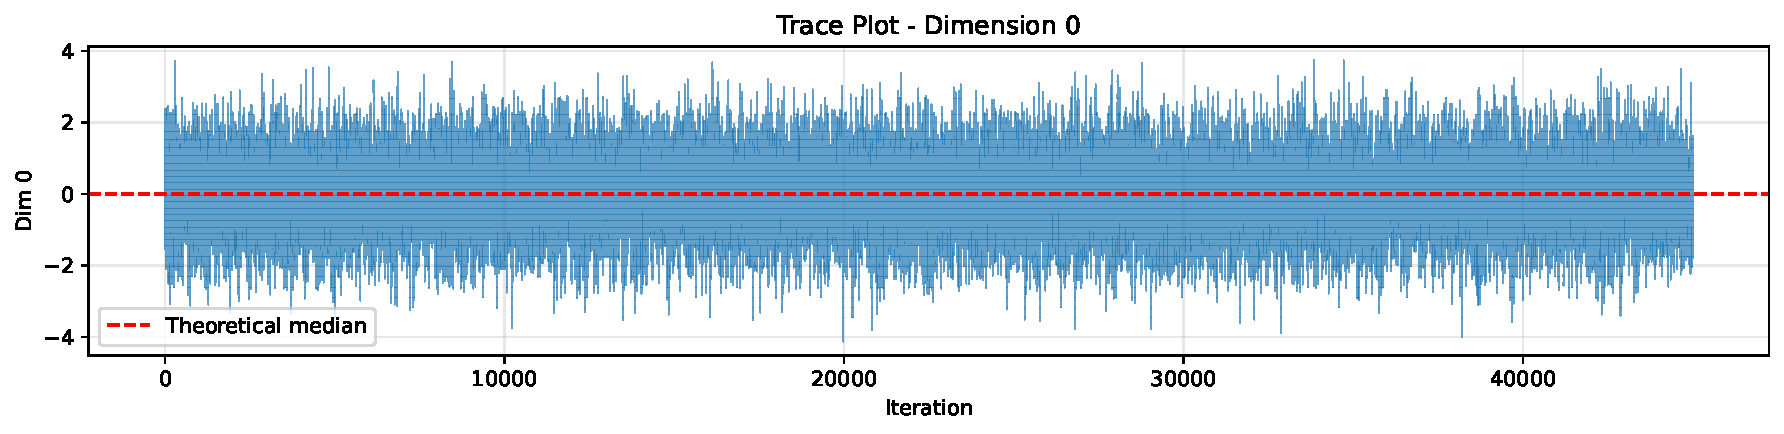
\includegraphics[width=\textwidth]{../../experiments/figures/original_thesis/case_studies/01_mala_gaussian_gold_standard_trace}
  \caption{Trace plot.}
\end{subfigure}\\[1ex]
\begin{subfigure}{0.42\textwidth}
  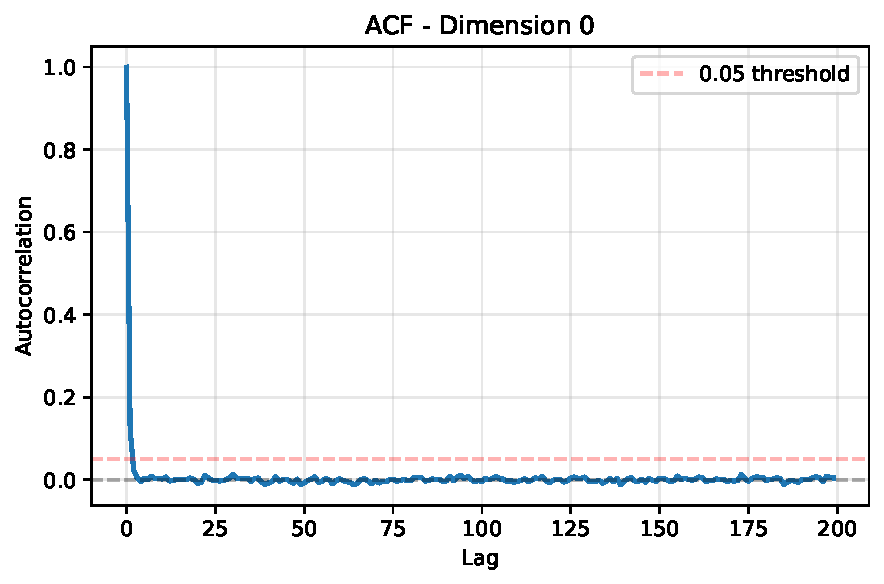
\includegraphics[width=\textwidth]{../../experiments/figures/original_thesis/case_studies/01_mala_gaussian_gold_standard_acf}
  \caption{Αυτοσυσχέτιση.}
\end{subfigure}\hfill
\begin{subfigure}{0.55\textwidth}
  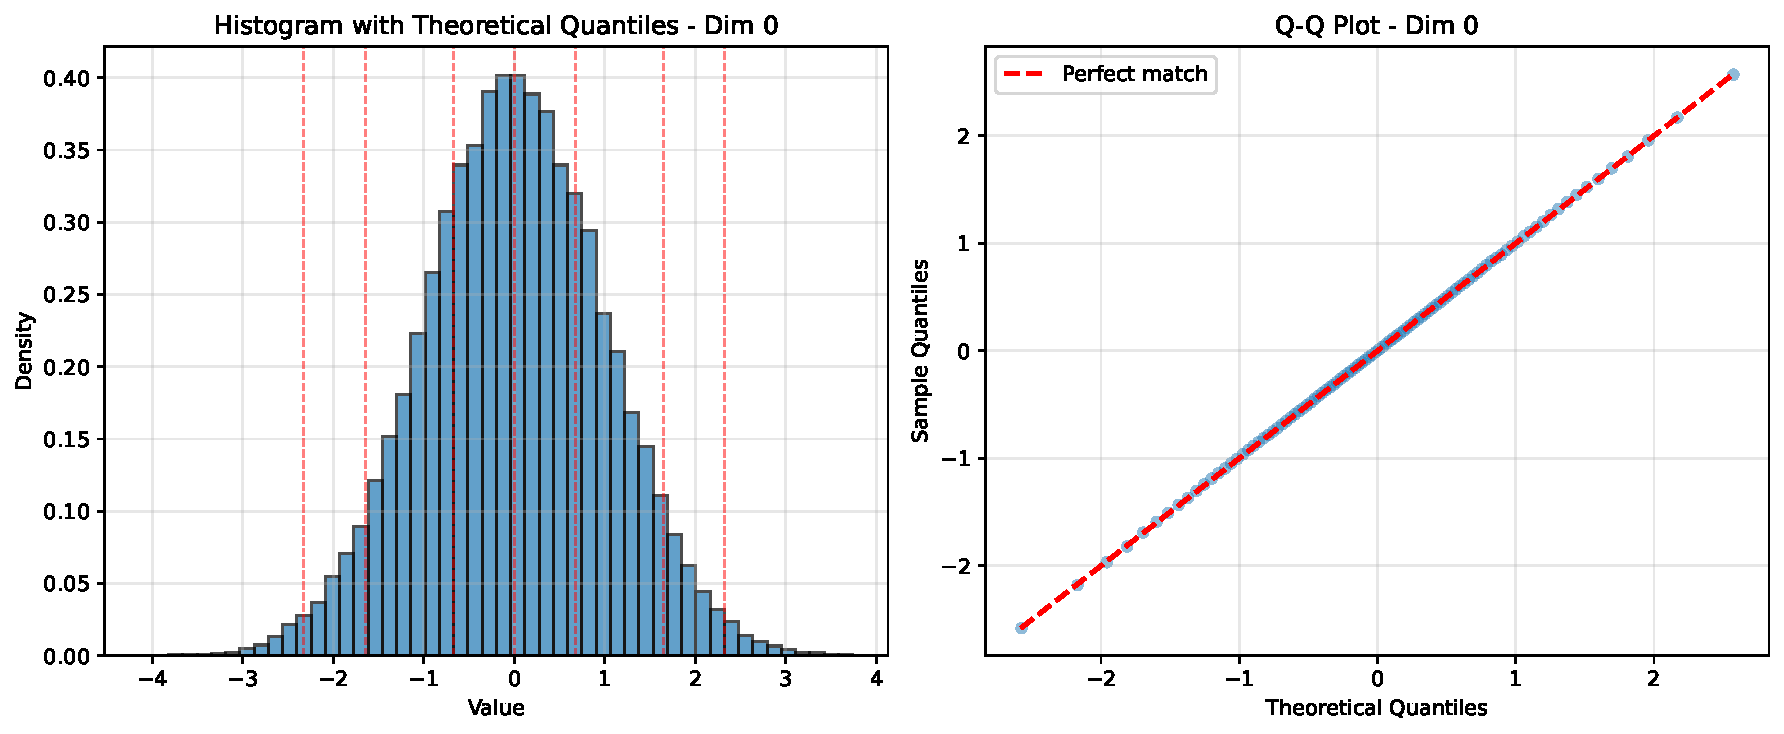
\includegraphics[width=\textwidth]{../../experiments/figures/original_thesis/case_studies/01_mala_gaussian_gold_standard_gof}
  \caption{Ιστόγραμμα με θεωρητικά ποσοστημόρια (αριστερά) και Q-Q plot (δεξιά).}
\end{subfigure}
\caption{Μελέτη Περίπτωσης 1: MALA στη Γκαουσιανή κατανομή-στόχο. Συμπεριφορά αναφοράς για σύγκριση με τις υπόλοιπες περιπτώσεις.}
\label{fig:case-mala-gauss}
\end{figure}

 Το trace plot κινείται ελεύθερα γύρω από το μηδέν χωρίς τάση ή
  αργή εκκίνηση. Η αυτοσυσχέτιση πέφτει κάτω από $0.05$ σε λίγα
  μόνο βήματα, πράγμα που σημαίνει ότι διαδοχικά δείγματα είναι
  σχεδόν ανεξάρτητα --- εξ ου και το υψηλό ESS $\approx 36{,}000$.
  Το Q-Q plot ακολουθεί τη διαγώνιο σε όλο το εύρος, και το
  ιστόγραμμα εφαρμόζει καλά στη θεωρητική Γκαουσιανή πυκνότητα.
  Οι υπόλοιπες μελέτες περίπτωσης θα πρέπει να διαβάζονται ως
  αποκλίσεις από αυτή την εικόνα.


\subsection{Μελέτη Περίπτωσης 2 --- ULA Γκαουσιανή (ήπιo bias διακριτοποίησης)}
\label{sec:case-ula-gauss}

\begin{figure}[H]
\centering
\begin{subfigure}{\textwidth}
  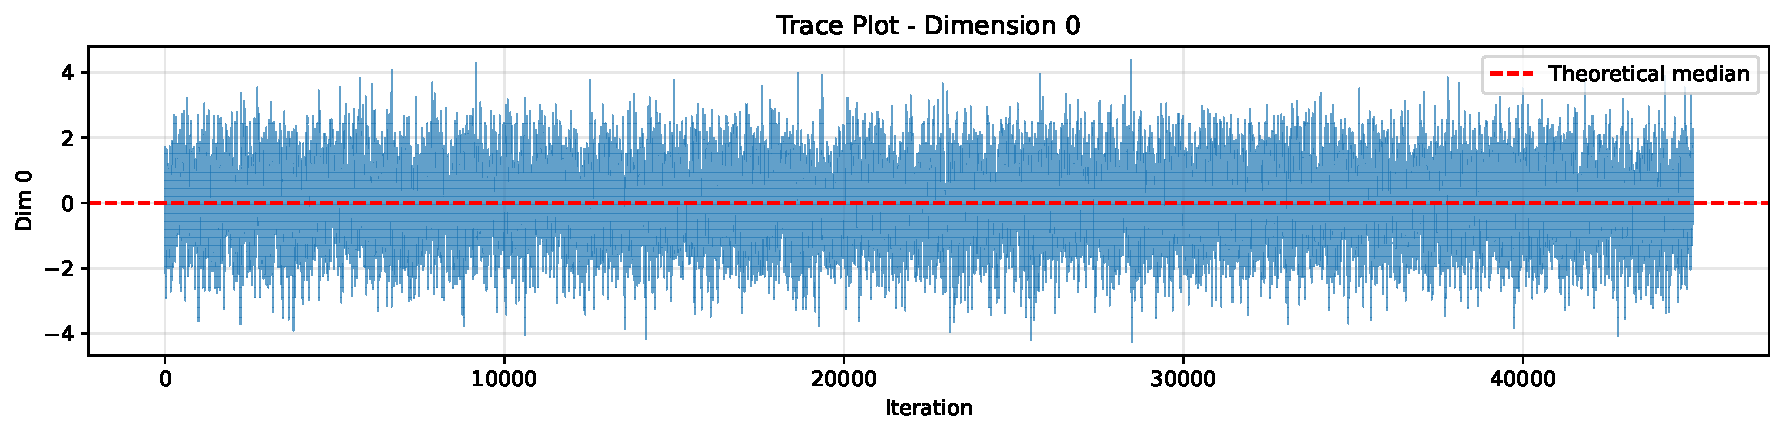
\includegraphics[width=\textwidth]{../../experiments/figures/original_thesis/case_studies/02_ula_gaussian_mild_bias_trace}
  \caption{Trace plot.}
\end{subfigure}\\[1ex]
\begin{subfigure}{0.42\textwidth}
  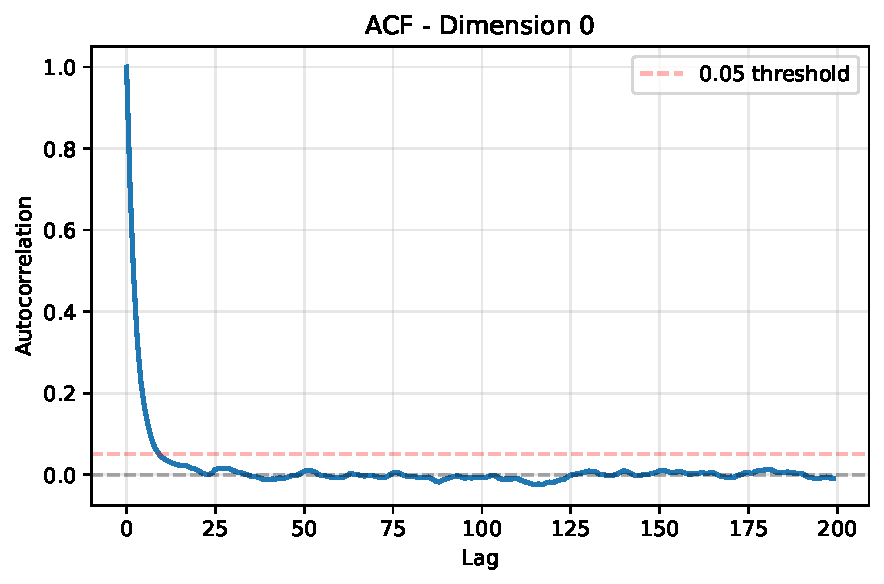
\includegraphics[width=\textwidth]{../../experiments/figures/original_thesis/case_studies/02_ula_gaussian_mild_bias_acf}
  \caption{Αυτοσυσχέτιση.}
\end{subfigure}\hfill
\begin{subfigure}{0.55\textwidth}
  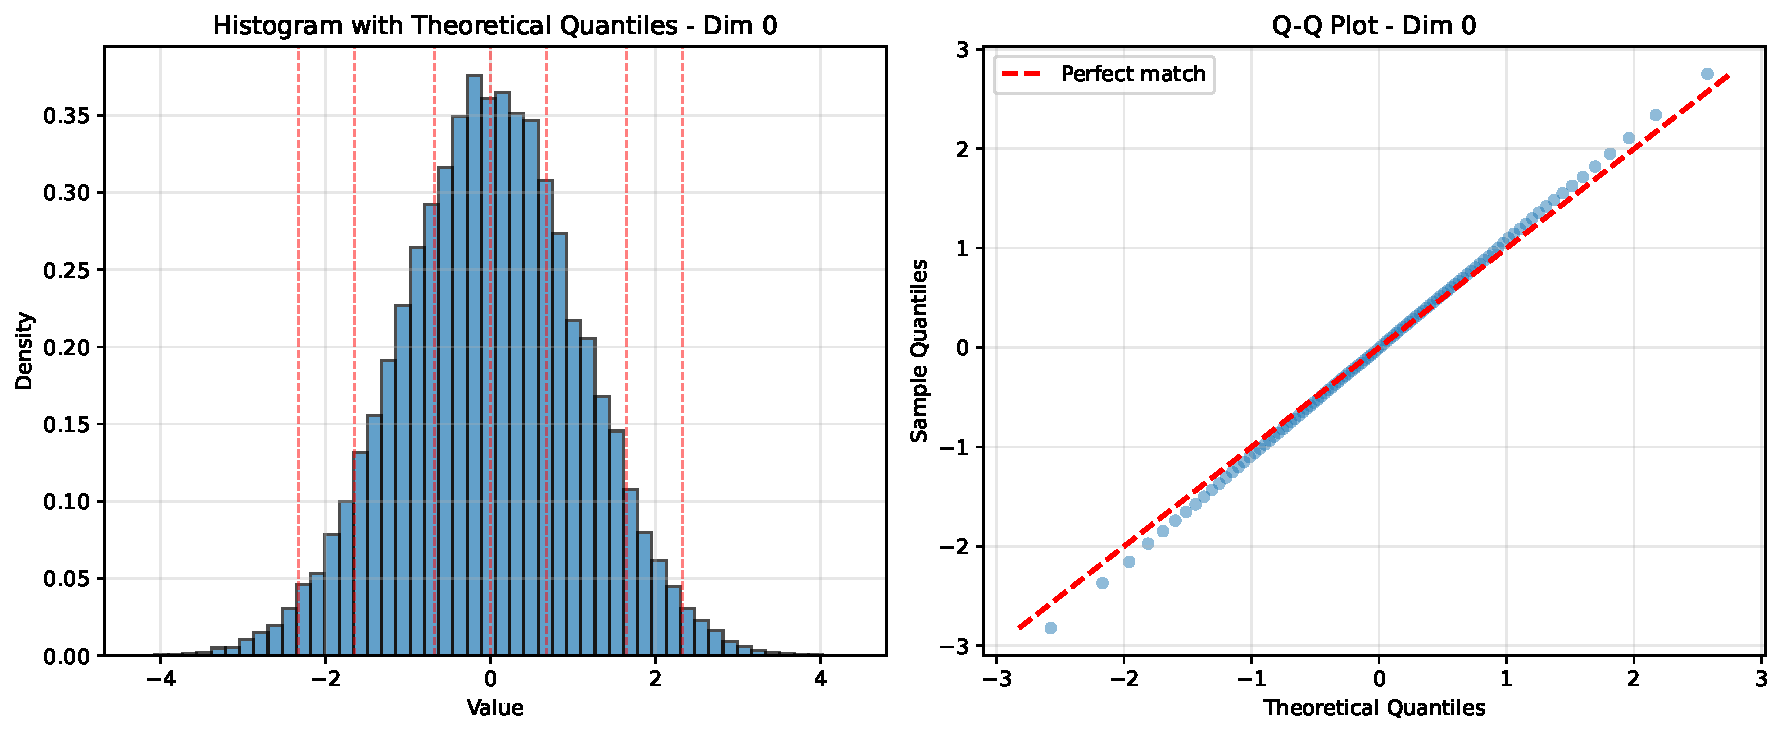
\includegraphics[width=\textwidth]{../../experiments/figures/original_thesis/case_studies/02_ula_gaussian_mild_bias_gof}
  \caption{Ιστόγραμμα και Q-Q plot.}
\end{subfigure}
\caption{Μελέτη Περίπτωσης 2: ULA στη Γκαουσιανή κατανομή-στόχο σε $\eta=0.30$.
Η αλυσίδα αναμειγνύεται καλά (το trace plot και η ACF φαίνονται κανονικά) αλλά
η στάσιμη κατανομή είναι ελαφρώς πλατύτερη από την κατανομή-στόχο.}
\label{fig:case-ula-gauss}
\end{figure}

Εξωτερικά αυτή η περίπτωση φαίνεται πανομοιότυπη με την Περίπτωση 1: το trace
plot είναι αυτό μιας υγιούς αλυσίδας και η ACF πέφτει καθαρά στο μηδέν έως
για lag $\sim 7$. Η μεροληψία εμφανίζεται μόνο στο πλαίσιο καλής προσαρμογής.
Το εμπειρικό ιστόγραμμα εκτείνεται ορατά πέραν των δεικτών θεωρητικού
ποσοστημορίου $97.5\%$ (στο $\pm 1.96$). Το Q-Q plot κάμπτεται ελαφρώς προς τα
έξω στα άκρα, υποδηλώνοντας ότι το εμπειρικό ποσοστημόριο $97.5\%$ της
αλυσίδας είναι ελαφρώς πιο ακραίο από το αναλυτικό. Η αλυσίδα αναμειγνύεται
αποδοτικά --- προς μια στάσιμη κατανομή ελαφρώς πλατύτερη από την
κατανομή-στόχο. Αυτό αποτελεί το χαρακτηριστικό αποτύπωμα της στατικής μεροληψίας
$\mathcal{O}(\eta)$ του ULA: μια αλυσίδα που φαίνεται υγιής βάσει διαγνωστικών
ανάμειξης αλλά της οποίας τα διαγνωστικά αντιστοίχισης κατανομής αποκαλύπτουν
το σφάλμα.

\subsection{Μελέτη Περίπτωσης 3 --- ULA Cauchy (κατάρρευση βαριάς ουράς)}
\label{sec:case-ula-cauchy}

\begin{figure}[H]
\centering
\begin{subfigure}{\textwidth}
  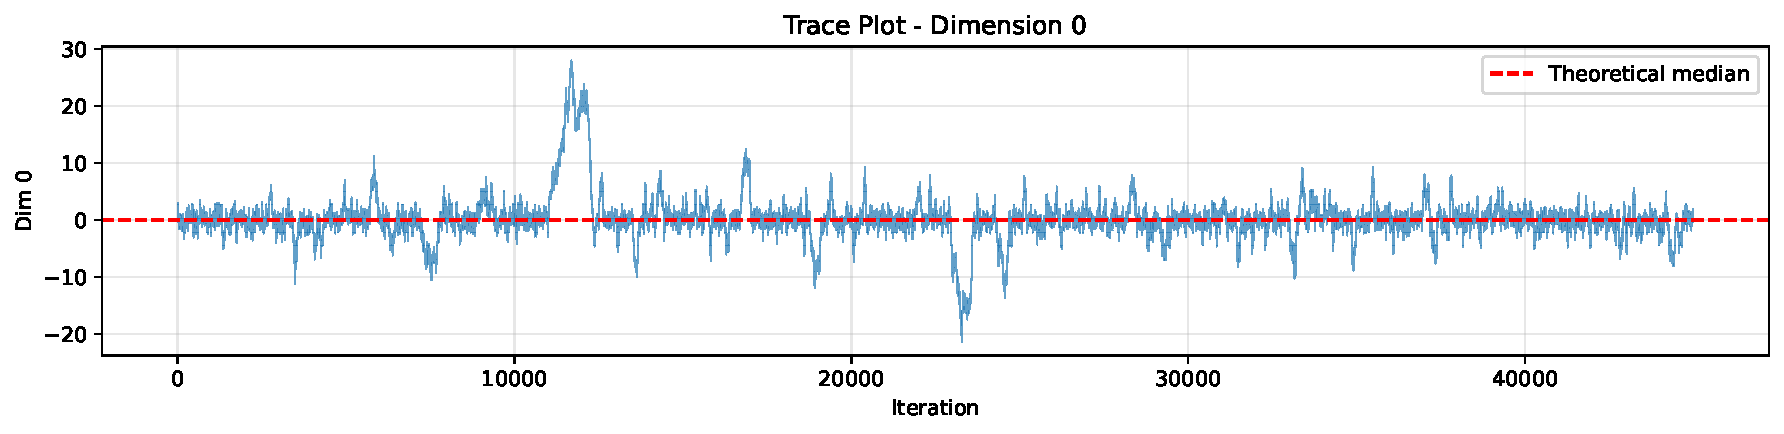
\includegraphics[width=\textwidth]{../../experiments/figures/original_thesis/case_studies/03_ula_cauchy_tail_collapse_trace}
  \caption{Trace plot.}
\end{subfigure}\\[1ex]
\begin{subfigure}{0.42\textwidth}
  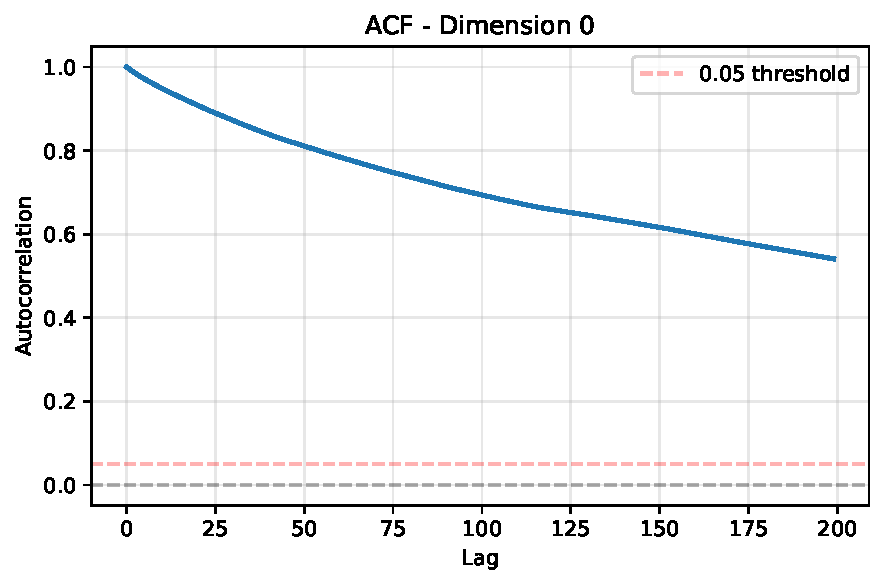
\includegraphics[width=\textwidth]{../../experiments/figures/original_thesis/case_studies/03_ula_cauchy_tail_collapse_acf}
  \caption{Αυτοσυσχέτιση.}
\end{subfigure}\hfill
\begin{subfigure}{0.55\textwidth}
  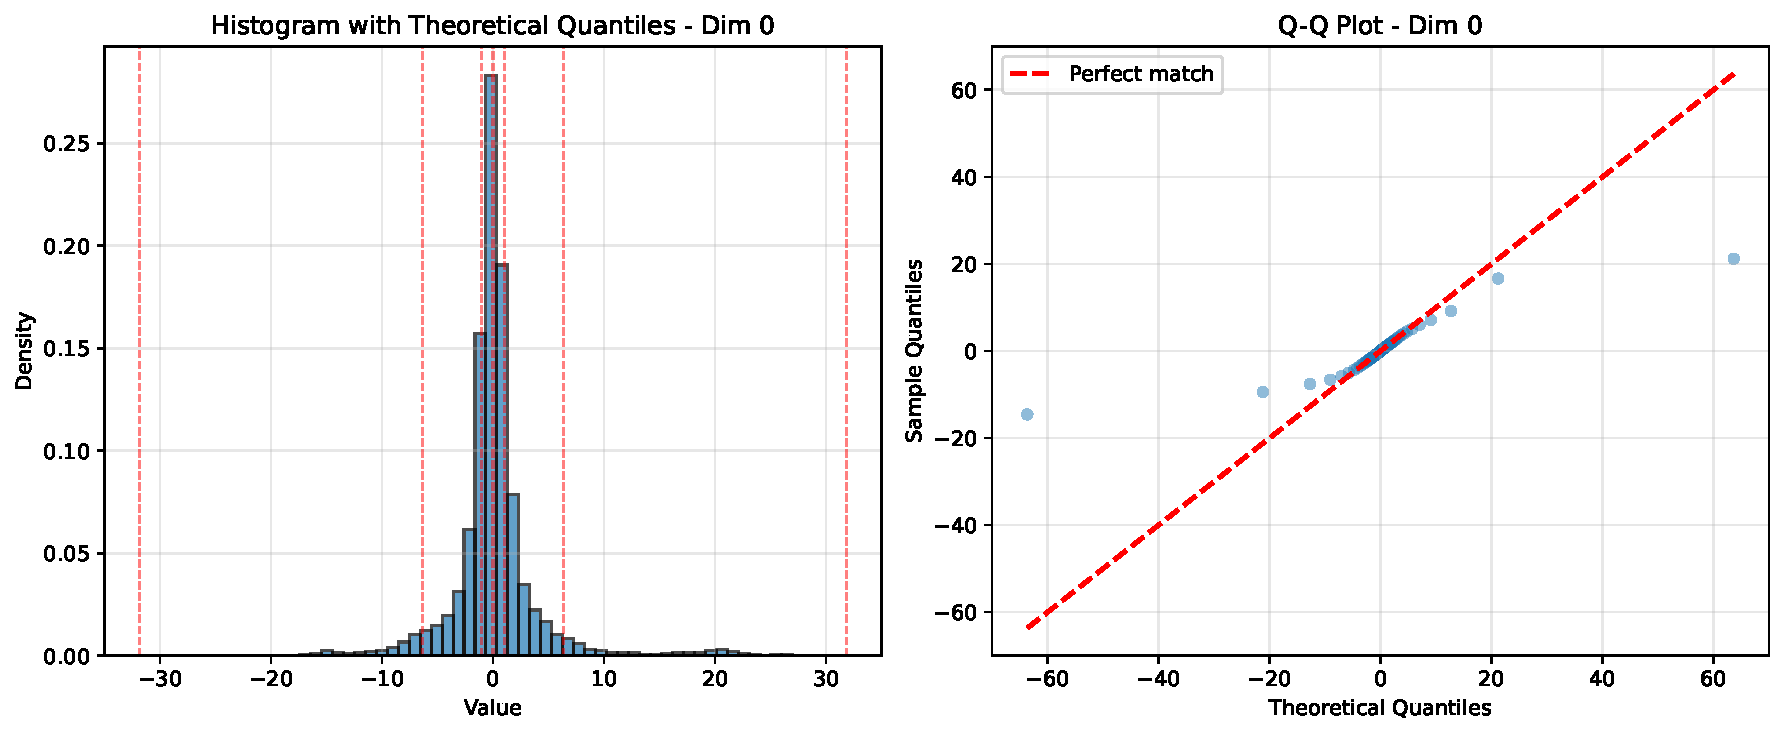
\includegraphics[width=\textwidth]{../../experiments/figures/original_thesis/case_studies/03_ula_cauchy_tail_collapse_gof}
  \caption{Ιστόγραμμα και Q-Q plot. Οι κατακόρυφες κόκκινες γραμμές σηματοδοτούν
  τα θεωρητικά ποσοστημόρια $1\%$ και $99\%$ της Cauchy στο $\pm 31.8$.}
\end{subfigure}
\caption{Μελέτη Περίπτωσης 3: ULA στην Cauchy κατανομή-στόχο σε $\eta=0.10$.
Η αλυσίδα φτάνει στο $|x|\approx 20$ σε περιστασιακές εκδρομές αλλά δεν μπορεί
να φτάσει σε μεγαλύτερες τιμές τα θεωρητικά ποσοστημόρια $1\%/99\%$ της Cauchy είναι στο
$\pm 31.8$.}
\label{fig:case-ula-cauchy}
\end{figure}

Αυτή είναι η κεντρική αποτυχία που τεκμηριώνεται στην εργασία. Το trace
plot δείχνει απομονωμένες εκδρομές από την αρχή που φτάνουν στο $|x| \approx 20$,
αλλά τα θεωρητικά ποσοστημόρια $1\%$ και $99\%$ της Cauchy βρίσκονται στο
$\pm 31.8$ --- η αλυσίδα απλώς δεν φτάνει εκεί σε $45{,}000$ δείγματα μετά το
burn-in. Το Q-Q plot φανερώνει το πρόβλημα καθαρά: τα πιο ακραία εμπειρικά
ποσοστημόρια στην αλυσίδα είναι πολύ μικρότερα (σε απόλυτη τιμή) από τα
αντίστοιχα θεωρητικά ποσοστημόρια. Η συνάρτηση αυτοσυσχέτισης καθιστά ρητή
την παθολογία ανάμειξης: σε υστέρηση $200$ η αυτοσυσχέτιση παραμένει γύρω στο
$0.5$, πολύ πάνω από το κατώφλι $0.05$ --- η αλυσίδα εξερευνά αργά ακόμη και
εντός της περιοχής που φτάνει.

Ο μηχανισμός είναι εκείνος που περιγράφεται στην Ενότητα~\ref{sec:tail-correlation}:
για το δυναμικό Cauchy, η ντετερμινιστική ολίσθηση της πρότασης ULA
$-\eta \nabla U(x)$ τείνει στο μηδέν καθώς $\|x\|\to\infty$, οπότε η αλυσίδα
δεν έχει τρόπο να μεροληπτεί είτε \emph{προς} είτε \emph{μακριά από} τις βαθιές
ουρές. Με θόρυβο πρότασης τάξης $\sqrt{2\eta} \approx 0.45$, η αναμενόμενη
μετατόπιση ανά βήμα είναι πολύ μικρότερη από την έκταση που καλύπτουν οι ουρές της κατανομής.

\subsection{Μελέτη Περίπτωσης 4 --- BAOAB Cauchy (καλύτερη διαχείριση βαριάς ουράς)}
\label{sec:case-baoab-cauchy}

\begin{figure}[H]
\centering
\begin{subfigure}{\textwidth}
  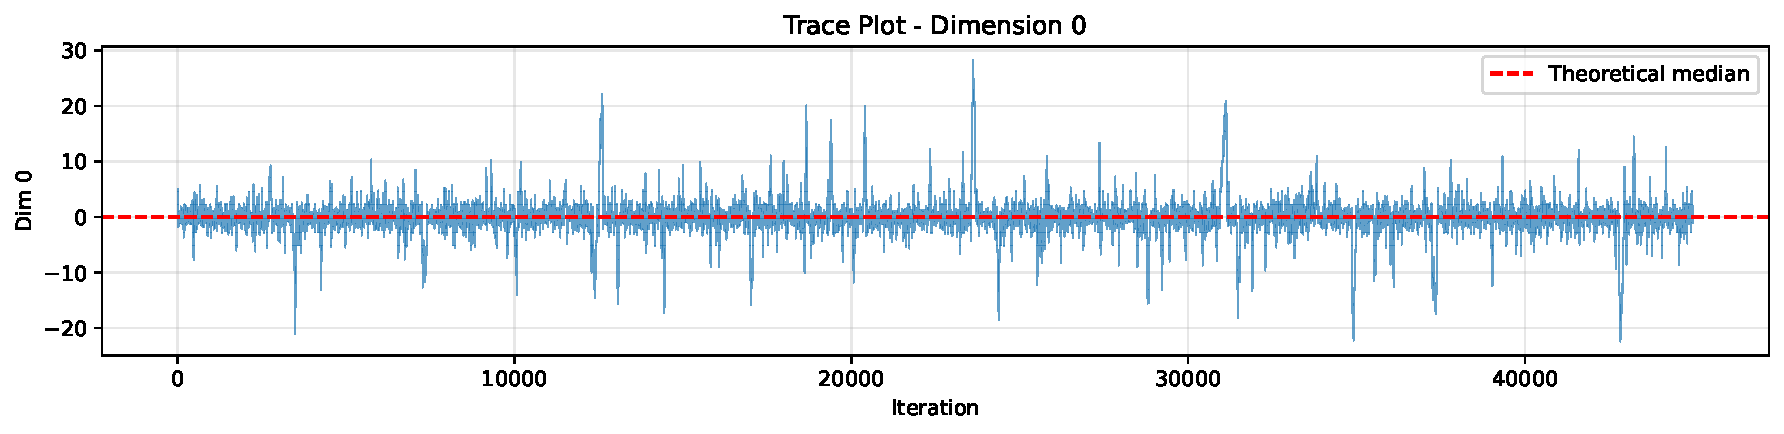
\includegraphics[width=\textwidth]{../../experiments/figures/original_thesis/case_studies/04_baoab_cauchy_best_trace}
  \caption{Trace plot. Σημειώστε τις μεγαλύτερες εκδρομές σε σύγκριση με την Περίπτωση 3.}
\end{subfigure}\\[1ex]
\begin{subfigure}{0.42\textwidth}
  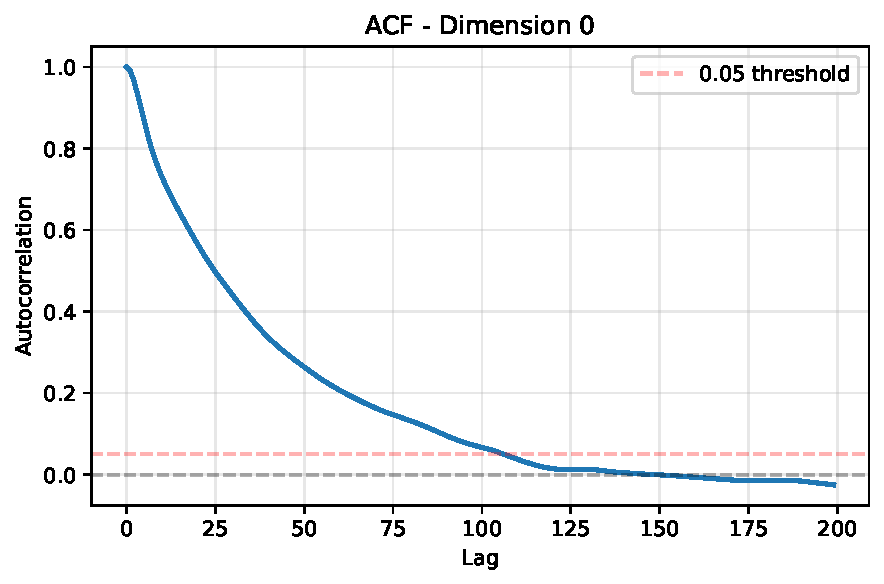
\includegraphics[width=\textwidth]{../../experiments/figures/original_thesis/case_studies/04_baoab_cauchy_best_acf}
  \caption{Αυτοσυσχέτιση.}
\end{subfigure}\hfill
\begin{subfigure}{0.55\textwidth}
  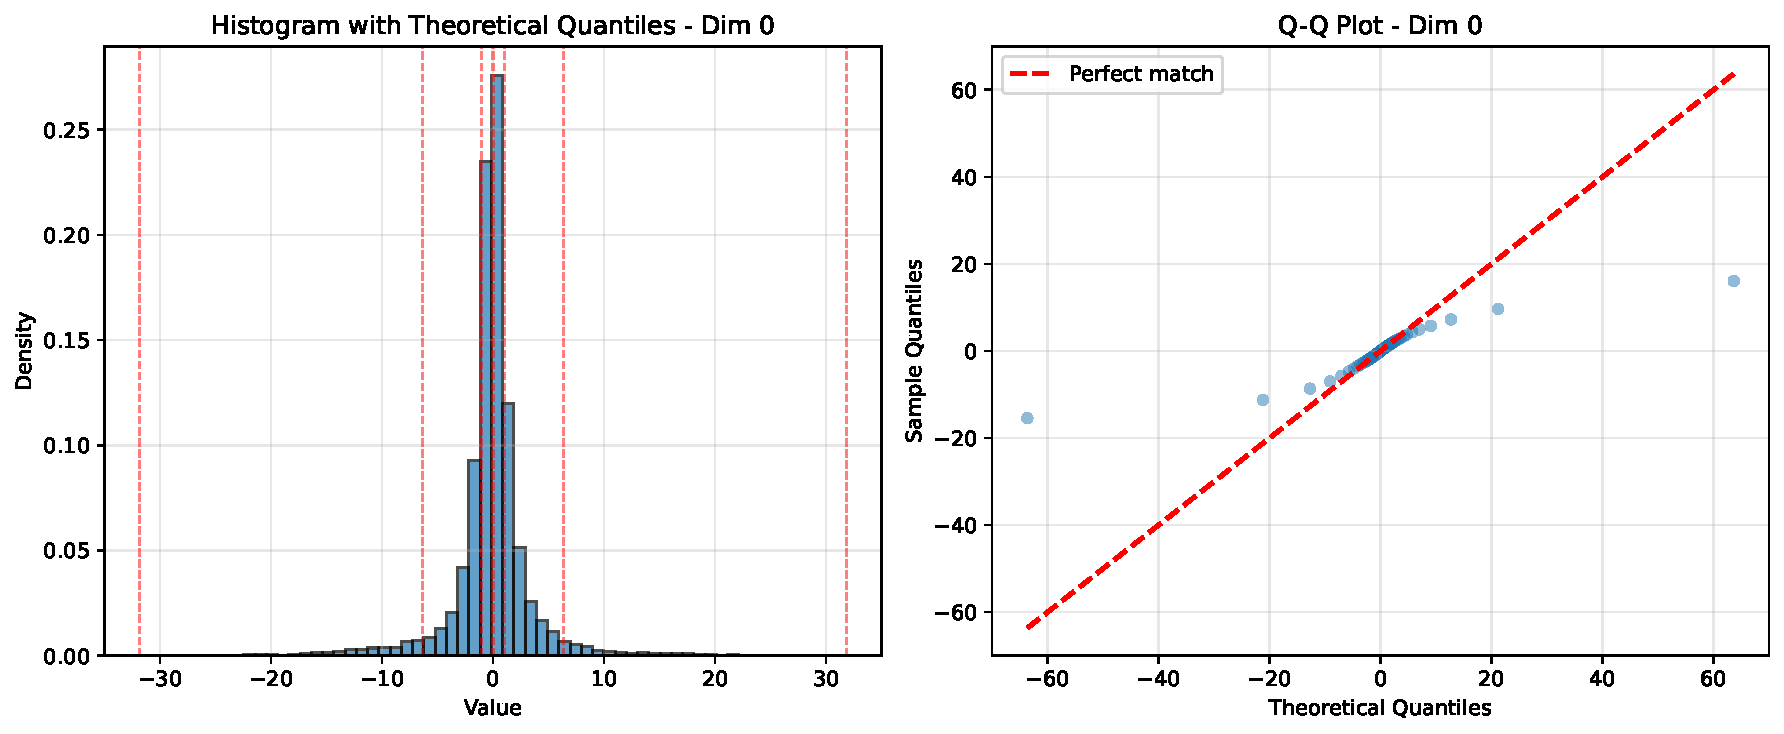
\includegraphics[width=\textwidth]{../../experiments/figures/original_thesis/case_studies/04_baoab_cauchy_best_gof}
  \caption{Ιστόγραμμα και Q-Q plot.}
\end{subfigure}
\caption{Μελέτη Περίπτωσης 4: BAOAB στην Cauchy κατανομή-στόχο σε $\eta=0.5$,
$\gamma=0.5$. Το trace plot δείχνει εκδρομές στο $\pm 28$ --- κοντά στα θεωρητικά
ποσοστημόρια $1\%/99\%$ στο $\pm 31.8$ --- τα οποία ο ULA στην Περίπτωση 3 δεν
μπορούσε να επιτύχει.}
\label{fig:case-baoab-cauchy}
\end{figure}

Σε σύγκριση με την Περίπτωση 3 για την ίδια κατανομή-στόχο, το trace plot του
BAOAB δείχνει ορατά μεγαλύτερες εκδρομές, που φτάνουν στο $|x| \approx 28$. Το
Q-Q plot είναι αντίστοιχα πιο κοντά στη διαγώνιο, και το ιστόγραμμα έχει μάζα
πέραν του $|x|=20$ που ο ULA δεν είχε ουσιαστικά καθόλου. Τα βαθύτερα εμπειρικά
ποσοστημόρια εξακολουθούν να υπολείπονται των αναλυτικών ποσοστημορίων Cauchy
στο $|x|=63$ (το εμπειρικό ποσοστημόριο $0.5\%$), αλλά το χάσμα είναι πολύ
μικρότερο από εκείνο του ULA. Σε αυτό το μήκος αλυσίδας η ουρά εξερευνάται
μερικώς. Η μελέτη σύγκλισης στην Ενότητα~\ref{sec:convergence-study} δείχνει
ότι με μεγαλύτερη αλυσίδα ο BAOAB συνεχίζει να βελτιώνεται στην κάλυψη ουράς.

Η εξήγηση για το πλεονέκτημα του BAOAB έναντι του ULA στην Cauchy
είναι η αναλυτική ενημέρωση Ornstein--Uhlenbeck στην ορμή,
$V \mapsto e^{-\gamma\eta} V + \sqrt{1 - e^{-2\gamma\eta}}\,\xi$, η οποία
εισάγει θόρυβο στη μεταβλητή ταχύτητας αντί απευθείας στη θέση. Η συσσωρευμένη
ορμή μπορεί να οδηγεί τη θέση σε πολλά βήματα μισής ολίσθησης πριν αποσβεστεί
από το επόμενο O-βήμα, επιτρέποντας στην αλυσίδα να διανύσει μεγάλες αποστάσεις
χωρίς να απαιτείται ένα ξαφνικό μεγάλο άλμα σε μία μόνο επανάληψη. Ο ULA δεν έχει
σύζευξη ορμής και επομένως δεν μπορεί να συσσωρεύσει μετατόπιση μεταξύ
επαναλήψεων με αυτόν τον τρόπο.

\subsection{Μελέτη Περίπτωσης 5 --- MALA Cauchy σε $d=50$ (βαριές ουρές σε μέτρια διάσταση)}
\label{sec:case-mala-cauchy-d50}

Αυτή η περίπτωση χρησιμοποιεί τον ίδιο αλγόριθμο με την Περίπτωση 1 (MALA)
για την ίδια κατανομή-στόχο με τις Περιπτώσεις 3--4 (Cauchy), αλλά σε διάσταση
$d=50$ αντί για $d=1$. Το βέλτιστο $\eta$ στο $d=50$ είναι $1.0$ (έναντι $4.0$
στο $d=1$, δείχνοντας την εμπειρική κλιμάκωση βήματος που συζητείται στην
Ενότητα~\ref{sec:dim-scaling}). Αναφερόμενες μετρικές από τον
Πίνακα~\ref{tab:cases}: διάμεσος KS $0.16$, αποδοχή $0.77$, ESS $\approx 108$.

\begin{figure}[H]
\centering
\begin{subfigure}{\textwidth}
  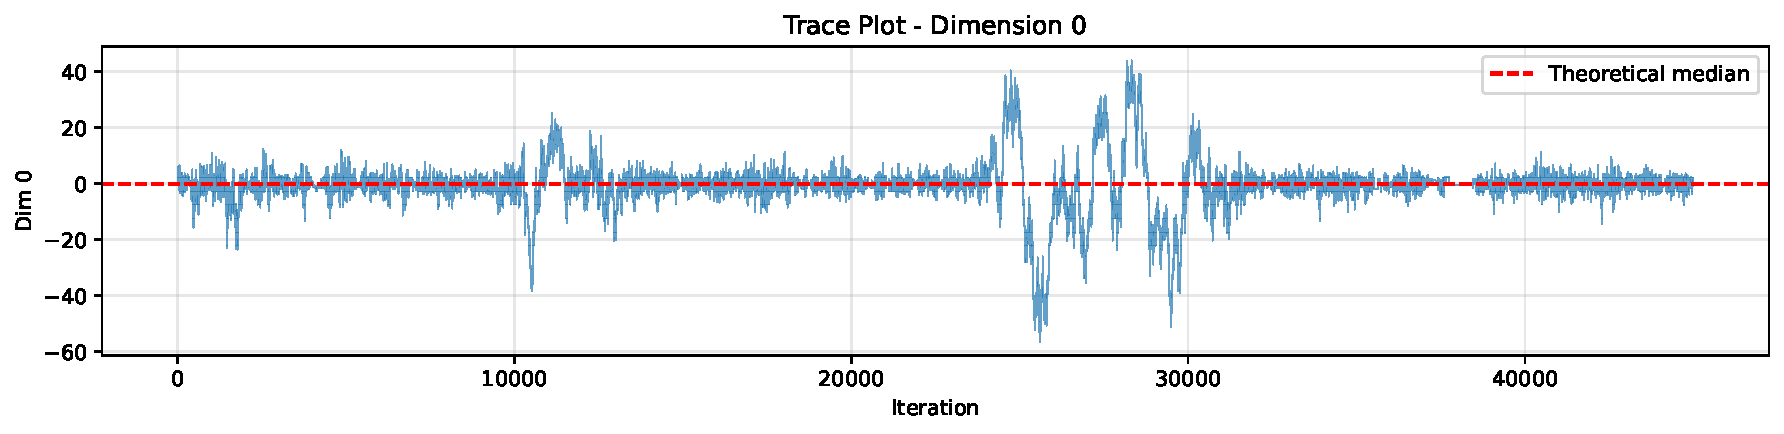
\includegraphics[width=\textwidth]{../../experiments/figures/original_thesis/case_studies/05_mala_cauchy_d50_trace}
  \caption{Trace plot.}
\end{subfigure}\\[1ex]
\begin{subfigure}{0.42\textwidth}
  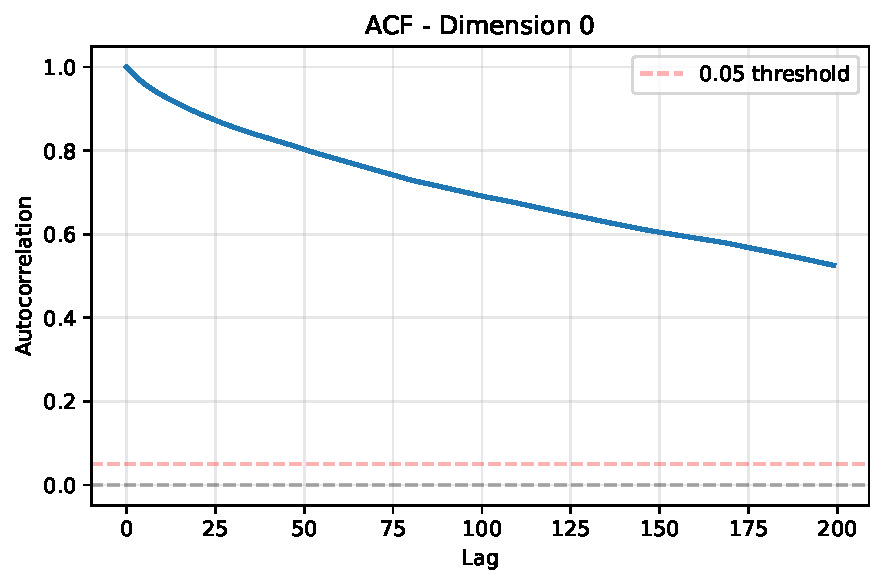
\includegraphics[width=\textwidth]{../../experiments/figures/original_thesis/case_studies/05_mala_cauchy_d50_acf}
  \caption{Αυτοσυσχέτιση.}
\end{subfigure}\hfill
\begin{subfigure}{0.55\textwidth}
  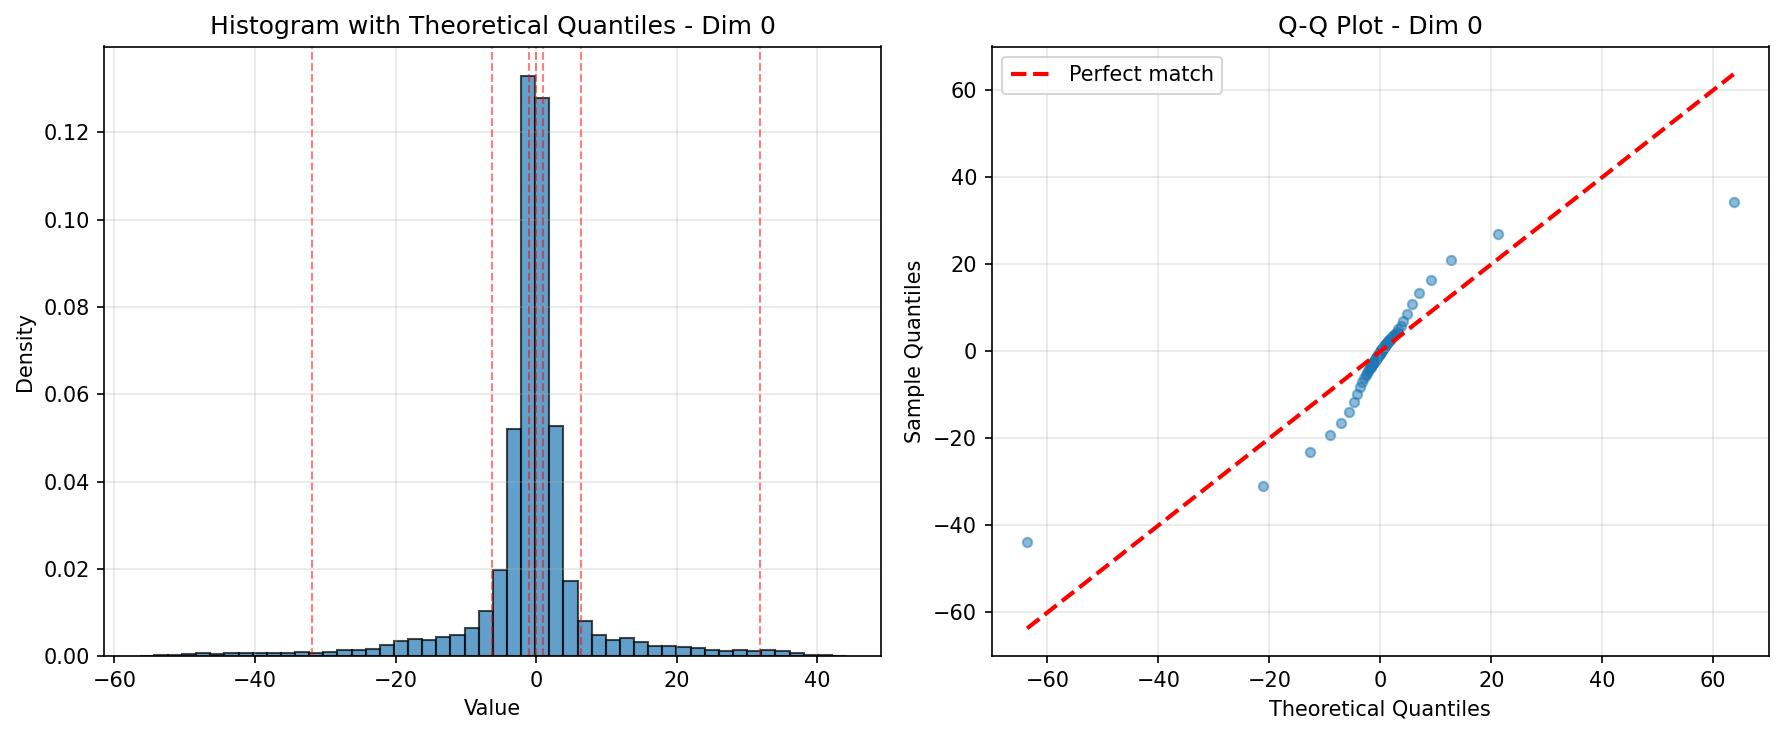
\includegraphics[width=\textwidth]{../../experiments/figures/original_thesis/case_studies/05_mala_cauchy_d50_gof}
  \caption{Ιστόγραμμα και Q-Q plot.}
\end{subfigure}
\caption{Μελέτη Περίπτωσης 5: MALA στην Cauchy κατανομή-στόχο σε $d=50$,
$\eta=1.0$. Η αλυσίδα φτάνει στο $|x| \approx 60$ σε περιστασιακές εκδρομές
αλλά περνά μακρά διαστήματα κοντά στην αρχή μεταξύ τους. Το ESS σε αυτή τη
διαμόρφωση είναι $\approx 108$ για $45{,}000$ δείγματα μετά το burn-in,
μείωση κατά τρεις τάξεις μεγέθους σε σύγκριση με τον MALA στη Γκαουσιανή κατανομή-στόχο για το ίδιο μήκος αλυσίδας.}
\label{fig:case-mala-cauchy-d50}
\end{figure}

Το trace plot δείχνει το ποιοτικό αποτύπωμα της δειγματοληψίας βαριάς ουράς
υψηλής διάστασης: μακρές ήσυχες περίοδοι κοντά στην αρχή που διακόπτονται από
σπάνιες εκρήξεις μεγάλων εκδρομών, με τις εκρήξεις να διαρκούν χιλιάδες
επαναλήψεις αντί για λίγα βήματα. Η συνάρτηση αυτοσυσχέτισης φθίνει πολύ πιο
αργά από οποιαδήποτε από τις άλλες μελέτες περίπτωσης, και το Q-Q plot δείχνει
μερική αλλά ελλιπή κάλυψη ουράς. Η αλυσίδα δεν έχει κολλήσει (αποδοχή $0.77$)
αλλά ο αποτελεσματικός χρόνος ανάμειξής της είναι δραματικά πιο αργός από ό,τι
στο $d=1$.

Η περίπτωση δείχνει το κεντρικό συμπέρασμα της
Ενότητας~\ref{sec:dim-dependence-tails}: η δειγματοληψία βαριάς ουράς σε μέτρια
διάσταση είναι ποιοτικά διαφορετική από τη δειγματοληψία βαριάς ουράς στο $d=1$.
Η στρατηγική προσαρμογής-μέσω-μεγαλύτερων-βημάτων του MALA συνεχίζει να
λειτουργεί αλλά με πολύ μειωμένη αποδοτικότητα δειγματοληψίας.

\subsection{Τι Δείχνουν οι Μελέτες Περίπτωσης}

Οι πέντε περιπτώσεις φανερώνουν τα ευρήματα των
προηγούμενων ενοτήτων. Η αντίθεση μεταξύ Περιπτώσεων 1 και 2 απομονώνει τη
μόνιμη μεροληψία του ULA σε ελαφριά κατανομή-στόχο: η αλυσίδα αναμειγνύεται καλά
αλλά στοχεύει σε μια ελαφρώς λανθασμένη κατανομή. Η αντίθεση μεταξύ Περιπτώσεων
2 και 3 απομονώνει την επίδραση της βαρύτητας ουράς στη συμπεριφορά του ULA: η
ίδια ήπια υπερ-κάλυψη στη Γκαουσιανή γίνεται πλήρης κατάρρευση ουράς στην
Cauchy, με την αυτοσυσχέτιση υστέρησης-100 να αυξάνεται από $\sim 0$ σε
$\sim 0.5$. Η αντίθεση μεταξύ Περιπτώσεων 3 και 4 απομονώνει τον ρόλο του
ολοκληρωτή: και οι δύο αλγόριθμοι είναι μεροληπτικοί (χωρίς έλεγχο Metropolis)
και στοχεύουν στην ίδια Cauchy, αλλά ο splitting ολοκληρωτής BAOAB επιτυγχάνει
ουσιαστικά καλύτερη εξερεύνηση ουράς από το απλό βήμα Euler του ULA. Τέλος, η
Περίπτωση 5 απομονώνει τον ρόλο της διάστασης: ο ίδιος αλγόριθμος (MALA) για
την ίδια κατανομή-στόχο (Cauchy) στο $d=50$ αντί για $d=1$ έχει την αποδοτικότητα
δειγματοληψίας του μειωμένη κατά τρεις τάξεις μεγέθους σε ESS.


\section{Μελέτη Σύγκλισης στις Βέλτιστες Διαμορφώσεις}
\label{sec:convergence-study}

\subsection{Σχεδιασμός}

Μια ξεχωριστή μελέτη αντιμετωπίζει το ερώτημα: καθώς αυξάνεται το μήκος
αλυσίδας, πώς εξελίσσονται τα διαγνωστικά; Εκτελούμε καθεμία από τις εννέα
βέλτιστες διαμορφώσεις (αλγόριθμος, κατανομή) από τον Πίνακα~\ref{tab:best-configs}
για $10^6$ επαναλήψεις και υπολογίζουμε τις μετρικές σε τέσσερα σημεία ελέγχου
$N \in \{5\!\cdot\!10^4, 10^5, 5\!\cdot\!10^5, 10^6\}$. Όπως στη μελέτη
πλέγματος, κάθε διαμόρφωση εκτελείται με $10$ ανεξάρτητες εκτελέσεις (η καθεμία
χρησιμοποιεί το ίδιο υπέρ-διεσπαρμένο σχήμα αρχικής κατάστασης που περιγράφεται
στην Ενότητα~\ref{sec:init-state}), και αναφέρουμε διάμεσο και IQR μεταξύ
εκτελέσεων σε κάθε σημείο ελέγχου. Το σημείο ελέγχου $5 \times 10^4$
αντιστοιχεί στο μήκος αλυσίδας της προηγούμενης μελέτης πλέγματος, οπότε το αριστερότερο σημείο κάθε καμπύλης σύγκλισης συμπίπτει με την αντίστοιχη γραμμή του
Πίνακα~\ref{tab:best-configs}. Το σημείο ελέγχου $10^6$ είναι είκοσι φορές
μεγαλύτερο. Για μια αλυσίδα που δειγματοληπτεί σωστά, το KS θα
έπρεπε να φθίνει κατά $1/\sqrt{N}$ μεταξύ σημείων ελέγχου --- που στην
περίπτωσή μας θα αντιστοιχούσε σε μείωση κατά παράγοντα $\sqrt{20} \approx 4.5$
μεταξύ $5\times 10^4$ και $10^6$ επαναλήψεων, ισοδύναμη με αναλογία $0.224$.

\subsection{Σύγκλιση KS}

\begin{figure}[ht]
\centering
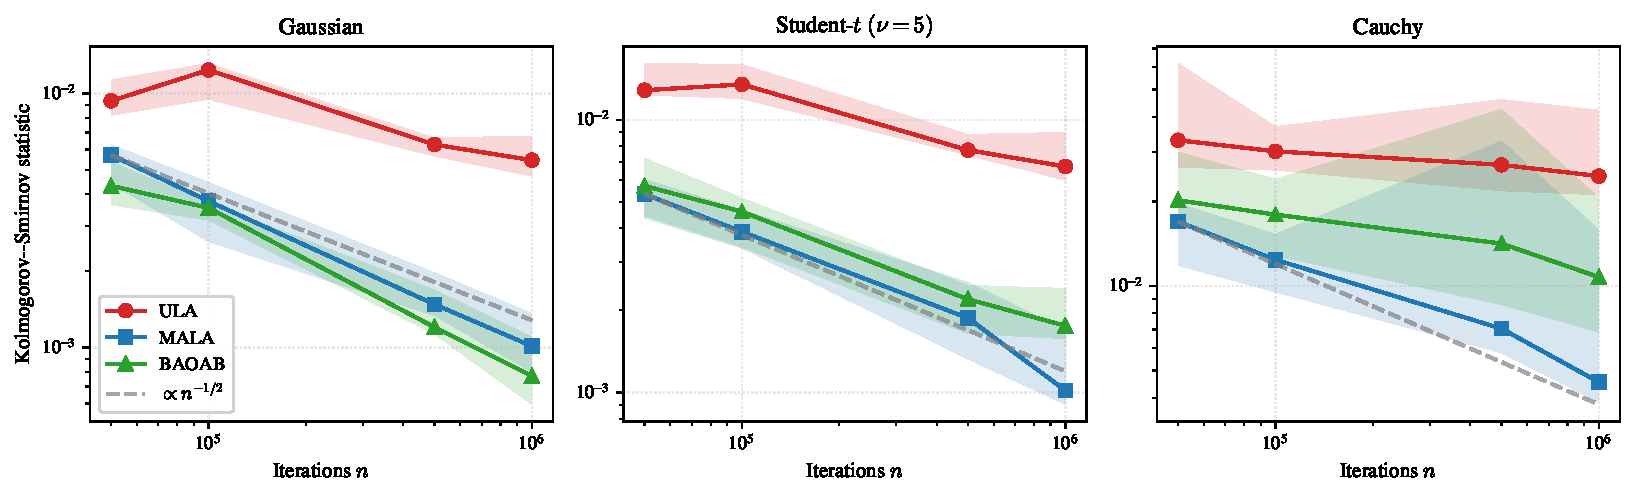
\includegraphics[width=\textwidth]{../../experiments/figures/original_thesis/ks_convergence}
\caption{Στατιστική Kolmogorov--Smirnov ως συνάρτηση του μήκους αλυσίδας, σε
λογαριθμική κλίμακα. Κάθε γραμμή είναι η διάμεση τιμή KS μεταξύ $10$ εκτελέσεων. Η
σκιασμένη ζώνη είναι το IQR. Η διακεκομμένη γκρι γραμμή είναι η κλίση αναφοράς
$N^{-1/2}$ που προβλέπεται από την κλασική θεωρία για αλυσίδα που στοχεύει
σωστά στην $\pi$.}
\label{fig:ks-conv}
\end{figure}

Ο Πίνακας~\ref{tab:ks-conv-ratio} συνοψίζει την αναλογία μείωσης μεταξύ ελάχιστου
και μέγιστου μήκους αλυσίδας. Υπενθυμίζουμε ότι $0.224$ είναι η ιδανική τιμή
$1/\sqrt{N}$.

\begin{table}[ht]
\centering
\small
\begin{tabular}{lccc}
\toprule
Αλγόριθμος & Γκαουσιανή & Student-$t$ & Cauchy \\
\midrule
ULA   & $0.58\times$ & $0.52\times$ & $0.75\times$ \\
MALA  & $\mathbf{0.18\times}$ & $\mathbf{0.19\times}$ & $\mathbf{0.27\times}$ \\
BAOAB & $\mathbf{0.18\times}$ & $0.31\times$ & $0.53\times$ \\
\bottomrule
\end{tabular}
\caption{Αναλογία μείωσης διαμέσου KS μεταξύ $N=5\times10^4$ και $N=10^6$.
Η κλασική πρόβλεψη $1/\sqrt{N}$ είναι $0.224\times$. Με έντονη γραφή
σηματοδοτούνται αναλογίες εντός παράγοντα δύο από την πρόβλεψη.}
\label{tab:ks-conv-ratio}
\end{table}

Η εικόνα είναι σαφής. Για τη Γκαουσιανή και τη Student-$t$ κατανομή-στόχο,
ο MALA και ο BAOAB επιτυγχάνουν αμφότεροι μειώσεις KS κοντά στον κλασικό ρυθμό
$1/\sqrt{N}$ --- δηλαδή η μετρική κυριαρχείται από τυχαίο σφάλμα Monte Carlo και
όχι από αλγοριθμική μεροληψία. Η KS του ULA πέφτει μεν, αλλά με πολύ πιο αργό
ρυθμό, υποδηλώνοντας ότι η μεροληψία του γίνεται η κυρίαρχη πηγή σφάλματος:
μακρύτερες αλυσίδες μειώνουν κατά μέσο όρο το τυχαίο σφάλμα αλλά δεν μπορούν
να αφαιρέσουν το κατώφλι μεροληψίας. Για την Cauchy, ο MALA συνεχίζει να
συγκλίνει κοντά στον ρυθμό $1/\sqrt{N}$, ο BAOAB σε περίπου τον μισό αυτόν τον
ρυθμό, και ο ULA μόλις κινείται πάνω από την εικοσαπλάσια αύξηση μεγέθους
δείγματος.

Οι απόλυτες τιμές KS στο $N = 10^6$ είναι: Γκαουσιανή --- BAOAB $0.0008$,
MALA $0.0010$, ULA $0.0055$. Student-$t$ --- MALA $0.0010$, BAOAB $0.0018$,
ULA $0.0067$. Cauchy --- MALA $0.0046$, BAOAB $0.0108$, ULA $0.0246$. Η Cauchy
είναι πραγματικά δύσκολη: στις $10^6$ επαναλήψεις ο MALA και ο BAOAB έχουν
τιμές KS κοντά στο σημείο που είχαν ο MALA και ο BAOAB στη Γκαουσιανή στις
$5\times 10^4$ επαναλήψεις.

\subsection{Κλιμάκωση ESS}

Το ESS θα πρέπει να αυξάνεται γραμμικά με το μήκος αλυσίδας εάν η αλυσίδα
βρίσκεται σε σταθερή-κατάσταση ανάμειξης. Το Σχήμα~\ref{fig:ess-scaling}
απεικονίζει το ESS ως συνάρτηση του $N$. Μια αλυσίδα που αναμειγνύεται με
σταθερό ρυθμό παράγει ευθεία γραμμή κλίσης ένα στους λογαριθμικούς άξονες.
Η διακεκομμένη γραμμή είναι η κλίση αναφοράς γραμμική-σε-$N$.

\begin{figure}[ht]
\centering
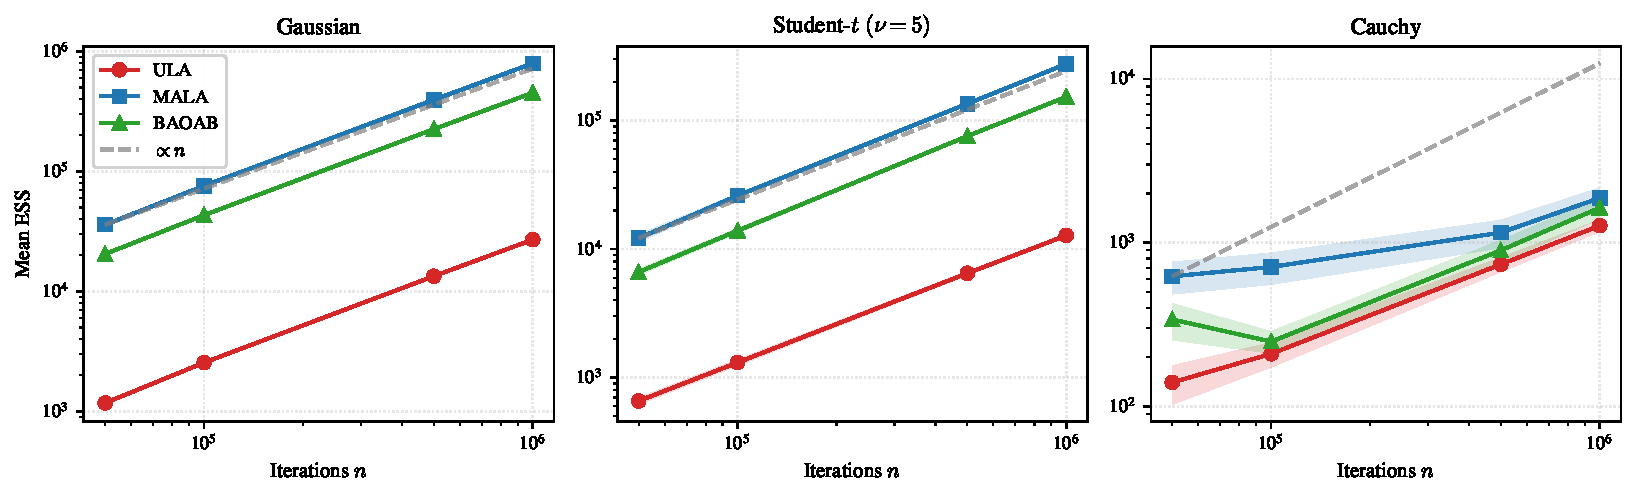
\includegraphics[width=\textwidth]{../../experiments/figures/original_thesis/ess_scaling}
\caption{Μέσο ESS ως συνάρτηση του μήκους αλυσίδας, διάμεση τιμή μεταξύ $10$
εκτελέσεων, με ζώνη $\pm$ τυπικό σφάλμα. Η διακεκομμένη γραμμή είναι η κλίση
αναφοράς γραμμική-σε-$N$.}
\label{fig:ess-scaling}
\end{figure}

Για τη Γκαουσιανή και τη Student-$t$, και οι τρεις αλγόριθμοι εκδηλώνουν
κλιμάκωση ESS κοντά στη γραμμική (αναλογία περίπου $20\times$ μεταξύ
$N=5\times 10^4$ και $N=10^6$). Για την Cauchy η κλιμάκωση είναι υπογραμμική:
μεταξύ των ίδιων δύο ακρών το ESS πολλαπλασιάζεται μόνο $3\times$ για τον MALA,
$5\times$ για τον BAOAB και $9\times$ για τον ULA. Η ερμηνεία είναι ότι
περιστασιακές μακρές εκδρομές στις ουρές της Cauchy κρατούν τον ολοκληρωμένο
χρόνο αυτοσυσχέτισης \emph{αυξανόμενο} με το μήκος αλυσίδας --- όσο μεγαλύτερη
η αλυσίδα, τόσο περισσότερες τέτοιες εκδρομές εμφανίζονται, και η καθεμία
διογκώνει τη συσχέτιση.

\subsection{Σύγκλιση q-MAE Ποσοστημορίου}

\begin{figure}[ht]
\centering
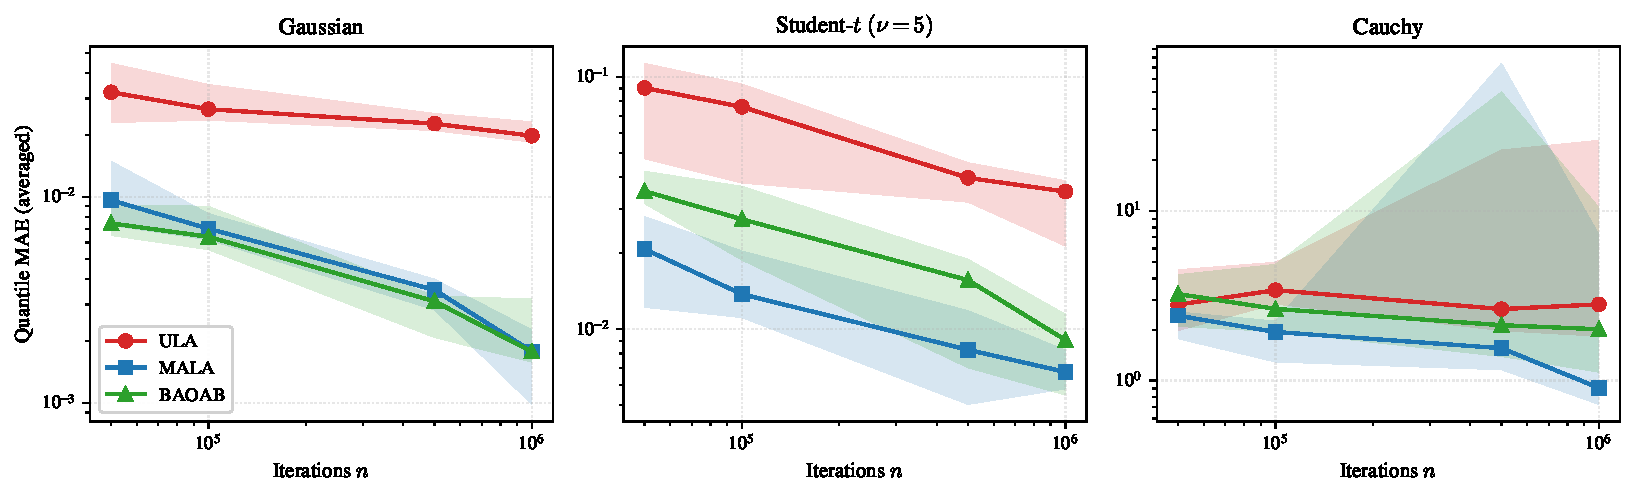
\includegraphics[width=\textwidth]{../../experiments/figures/original_thesis/quantile_mae_convergence}
\caption{Μέσο q-MAE ποσοστημορίου ως συνάρτηση του μήκους αλυσίδας, διάμεση τιμή
μεταξύ $10$ εκτελέσεων με ζώνη IQR.}
\label{fig:qmae-conv}
\end{figure}

Το q-MAE συμπεριφέρεται παρόμοια με το KS για τη Γκαουσιανή και τη Student-$t$:
ο MALA και ο BAOAB φθίνουν σταθερά, ο ULA ισοπεδώνεται. Για την Cauchy η εικόνα
είναι διαφορετική. Το q-MAE στις $10^6$ επαναλήψεις είναι $2.04$ για τον BAOAB,
$4.74$ για τον MALA και $4.81$ για τον ULA. \emph{Ο BAOAB έχει το καλύτερο q-MAE
για την Cauchy παρόλο που έχει υψηλότερο KS από τον MALA}: η στατιστική KS
κυριαρχείται από τον κορμό της κατανομής, αλλά το q-MAE στα άκρα κυριαρχείται
από το πόσο καλά φτάνει η αλυσίδα στις βαθιές ουρές. Ο BAOAB, χάρη στην ορμή του, καταγράφει καλύτερα τα ακραία ποσοστημόρια σε
σύγκριση με τον MALA, ο οποίος περιορίζεται από το ποσοστό αποδοχής. Η
επιλογή μεταξύ των δύο εξαρτάται από τις ανάγκες της εφαρμογής: αν
προτεραιότητα είναι η καλή προσαρμογή στον κορμό της κατανομής, ο MALA είναι
προτιμότερος για την Cauchy. Αν προτεραιότητα είναι η ακρίβεια στις ουρές,
ο BAOAB είναι προτιμότερος.

\subsection{Κάλυψη Ουράς Cauchy}

Η αναλογία κάλυψης ουράς είναι ο πιο καθαρός μεμονωμένος αριθμός που εκφράζει το πόσο
καλά φτάνει η αλυσίδα στις βαθιές ουρές της κατανομής-στόχου. Το
Σχήμα~\ref{fig:tail-cauchy} δείχνει την εξέλιξή της.

\begin{figure}[ht]
\centering
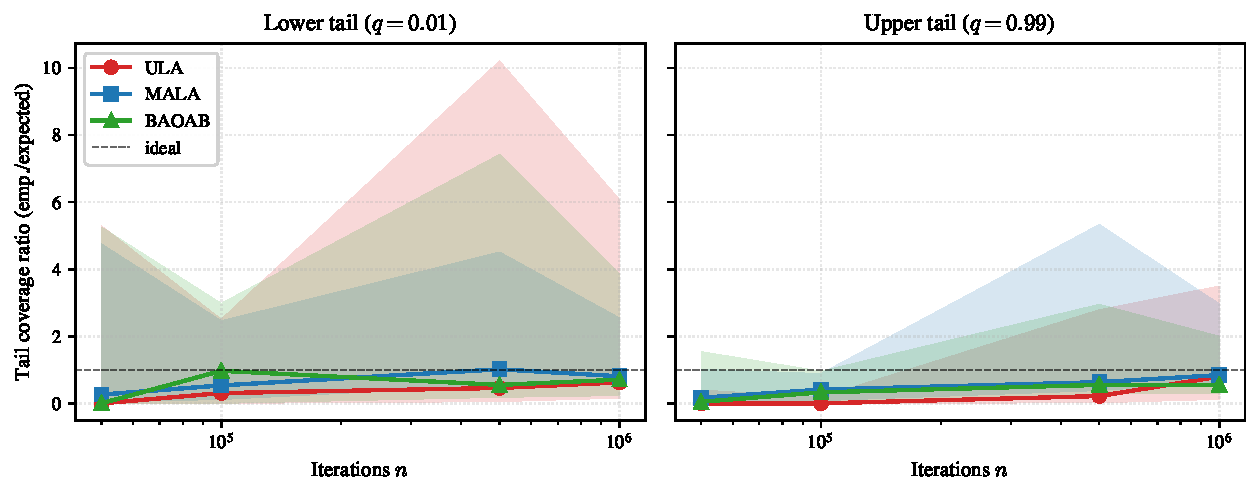
\includegraphics[width=\textwidth]{../../experiments/figures/original_thesis/cauchy_tail_coverage}
\caption{Αναλογίες κάλυψης ουράς Cauchy στα ποσοστημόρια $1\%$ και $99\%$,
διάμεση τιμή μεταξύ $10$ εκτελέσεων με ζώνη εκατοστημορίου $[5\%, 95\%]$. Η οριζόντια
γραμμή στο $1.0$ σηματοδοτεί ιδανική κάλυψη.}
\label{fig:tail-cauchy}
\end{figure}

Και οι τρεις αλγόριθμοι πλησιάζουν την ιδανική κάλυψη $1.0$ από κάτω καθώς η
αλυσίδα μεγαλώνει. Στις $N=10^6$ επαναλήψεις οι διάμεσες τιμές κάλυψης ουράς είναι: MALA
$0.81$ στο $q=0.01$ και $0.84$ στο $q=0.99$, BAOAB $0.71$ και $0.55$ αντίστοιχα, 
ULA $0.63$ και $0.80$. Ο MALA πλησιάζει περισσότερο την ιδανική κάλυψη, αλλά
οι ζώνες εκατοστημορίου $[5\%, 95\%]$ είναι πλατιές και για τους τρεις
αλγορίθμους --- ορισμένες εκτελέσεις δίνουν καλύψεις κοντά στο μηδέν, άλλοι πάνω
από τη μονάδα. Αυτή η μεταβλητότητα μεταξύ εκτελέσεων είναι εγγενής στην Cauchy:
οι εκτιμητές ακραίων ποσοστημορίων σε κατανομές βαριάς ουράς έχουν κατανομές
δειγματοληψίας βαριάς ουράς, και ακόμη και μια σωστά συμπεριφερόμενη αλυσίδα
παράγει άγρια διαφορετικές εκτιμήσεις κάλυψης ουράς μεταξύ διαφορετικών
εκτελέσεων.

Η οπτικοποίηση διασποράς εκτελέσεων στο Σχήμα~\ref{fig:seed-spread} το δείχνει
αυτό άμεσα: κάθε λεπτή γραμμή είναι η τροχιά KS μιας από τις δέκα εκτελέσεις ανά
αλγόριθμο για την Cauchy, ενώ η μέση τροχιά ανά αλγόριθμο αποδίδεται με έντονη γραμμή.
Η οικογένεια MALA έχει ένα σφιχτό κεντρικό σύμπλεγμα με λίγα ακραία σημεία.
Η οικογένεια BAOAB έχει ευρύτερη κεντρική διασπορά. Η οικογένεια ULA έχει τη
χαλαρότερη διασπορά από όλες.

\begin{figure}[ht]
\centering
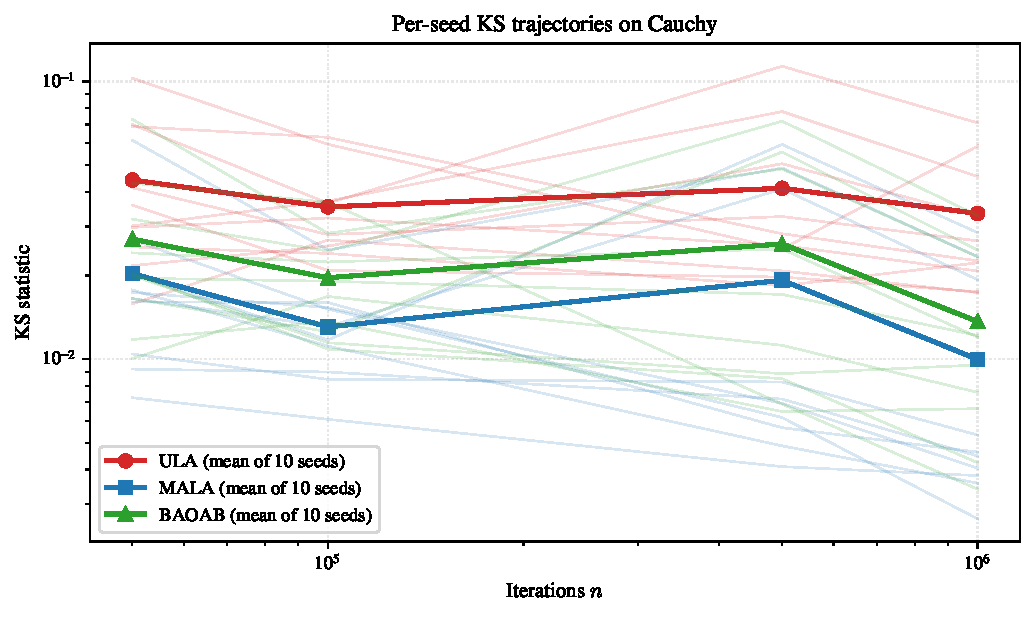
\includegraphics[width=0.75\textwidth]{../../experiments/figures/original_thesis/seed_spread_cauchy}
\caption{Τροχιές KS ανά εκτέλεση για την Cauchy κατανομή-στόχο. Οι αχνές γραμμές
αντιστοιχούν σε μεμονωμένες εκτελέσεις. Οι έντονες γραμμές είναι η μέση τροχιά
ανά αλγόριθμο.}
\label{fig:seed-spread}
\end{figure}

\subsection{Σύνοψη της Μελέτης Σύγκλισης}

Τρία συνοπτικά συμπεράσματα:

\begin{enumerate}
  \item Στα καθεστώτα ελαφριάς και μέτριας ουράς, ο MALA και ο BAOAB συγκλίνουν
        αμφότεροι κοντά στον γνωστό ρυθμό $1/\sqrt{N}$. Ο ULA κυριαρχείται από
        την μεροληψία διακριτοποίησης και συγκλίνει πολύ πιο αργά σε μια ελαφρώς
        λανθασμένη στάσιμη κατανομή.
  \item Για την Cauchy κατανομή-στόχο, ο MALA συνεχίζει να συγκλίνει κοντά στον
        ρυθμό $1/\sqrt{N}$. Ο BAOAB συγκλίνει περίπου με τον μισό αυτόν τον
        ρυθμό. Ο ULA μόλις κινείται. Από τους τρεις, ο MALA έχει τη χαμηλότερη
        απόλυτη KS στο $N=10^6$.
  \item Ωστόσο, το q-MAE της Cauchy στις $10^6$ επαναλήψεις ευνοεί τον BAOAB
        ($2.04$ έναντι $4.74$ του MALA), και η κάλυψη ουράς είναι παρόμοια μεταξύ
        των δύο. Η επιλογή βέλτιστου αλγορίθμου για την Cauchy εξαρτάται από το
        αν η εφαρμογή βαραίνει την προσαρμογή κορμού ή την ακρίβεια ουράς.
\end{enumerate}


\section{Επιφυλάξεις και Περιορισμοί}
\label{sec:caveats}

Κλείνουμε με κάποιες επιφυλάξεις που οριοθετούν τα συμπεράσματα αυτού του
κεφαλαίου.

\begin{enumerate}
 \item \emph{Είκοσι εκτελέσεις για τη μελέτη πλέγματος, δέκα για τη
        μελέτη σύγκλισης.} Ο αριθμός εκτελέσεων είναι αρκετός για να                                                          
        εντοπίσει μεγάλες διαφορές μεταξύ αλγορίθμων, αλλά όχι πολύ μικρές:
        διαφορές μικρότερες από $0.0005$ σε διάμεσο KS δεν είναι αξιόπιστες.
        Αρκετές συγκρίσεις BAOAB-έναντι-MALA στη Γκαουσιανή και τη
        Student-$t$ εμπίπτουν εντός αυτού του ορίου και θα πρέπει να
        θεωρούνται ισοπαλία.

  \item \emph{Η Cauchy δεν έχει πεπερασμένο μέσο ή διακύμανση.} Για τις
        εκτελέσεις Cauchy, οι μετρικές που βασίζονται σε μέσο και διακύμανση
        δεν έχουν νόημα και εμφανίζονται ως \texttt{NaN}. Η σύγκριση
        αλγορίθμων στην Cauchy γίνεται αποκλειστικά μέσω KS, διαμέσου και
        ποσοστημορίων.

  \item \emph{Το πλέγμα βήματος είναι διακριτό και εξαρτώμενο από την κατανομή.} Δοκιμάσαμε έναν
        συγκεκριμένο αριθμό τιμών $\eta$, οπότε το «βέλτιστο» που αναφέρουμε
        είναι το καλύτερο μέσα σε αυτό το πλέγμα, όχι το απόλυτο βέλτιστο.
        Για $d = 100$, μερικές από τις βέλτιστες τιμές βρίσκονται στο άκρο
        του πλέγματος --- κυρίως για BAOAB στη Γκαουσιανή και MALA στην
        Cauchy --- πράγμα που σημαίνει ότι μια ελαφρώς μεγαλύτερη ή
        μικρότερη τιμή $\eta$ θα μπορούσε να αποδώσει καλύτερα. Τα κύρια
        συμπεράσματα για τη συμπεριφορά των αλγορίθμων ως προς τη διάσταση
        δεν επηρεάζονται.

   \item \emph{Οι κατανομές-στόχοι είναι ισοτροπικές.} Και οι τρεις
        κατανομές-στόχοι αντιμετωπίζουν όλες τις διαστάσεις ισότιμα: δεν
        υπάρχουν διαστάσεις με διαφορετική κλίμακα ούτε συσχετίσεις μεταξύ
        τους. Στην πράξη, πολλά Bayesian προβλήματα δεν έχουν αυτή την
        ιδιότητα. Σε ανισοτροπικές κατανομές-στόχους η κατάταξη μεταξύ MALA
        και BAOAB μπορεί να αλλάξει, ειδικότερα το πλεονέκτημα ESS του BAOAB
        σε υψηλές διαστάσεις ενδέχεται να εξαφανιστεί χωρίς προρρύθμιση.

  \item \emph{Η μελέτη σύγκλισης είναι μόνο στο $d=1$.} Η μελέτη πλέγματος
        καλύπτει $d \in [1, 100]$ αλλά η μελέτη σύγκλισης που
        περιγράφεται στην Ενότητα~\ref{sec:convergence-study} διατηρεί $d=1$ για
        να απομονώσει τις επιδράσεις μήκους αλυσίδας από τις επιδράσεις
        διάστασης. Η παρατήρηση ότι και οι τρεις αλγόριθμοι καταρρέουν για την
        Cauchy μεταξύ $d=10$ και $d=100$ αποτελεί επομένως δήλωση σχετικά με
        ποιότητα αλυσίδας στις $5 \times 10^4$ επαναλήψεις. Μπορεί ή μπορεί να
        μην ισχύει εάν οι αλυσίδες τρέξουν πολύ περισσότερο σε υψηλό $d$.
 
\end{enumerate}

Παρά τους παραπάνω περιορισμούς, τα κύρια ευρήματα ισχύουν: ο ULA υποφέρει
από μόνιμη μεροληψία, ο MALA αποδίδει καλά σε όλες τις κατανομές, και ο BAOAB
κρατάει υψηλό ESS σε υψηλές διαστάσεις και καλύτερα ακραία ποσοστημόρια στις
βαριές ουρές.
% !TEX root = main.tex
\chapter{Συμπεράσματα και Συζήτηση}
\label{chap:conclusions}

Το κεφάλαιο αυτό συγκεντρώνει τα κύρια ευρήματα του
Κεφαλαίου~\ref{chap:experiments}, ελέγχει την υπόθεση της
Ενότητας~\ref{sec:intro-hypothesis}, δίνει μια σύσταση ανά πηγή δυσκολίας και
παραθέτει πιθανές κατευθύνσεις για μελλοντική έρευνα.

\section{Επανεξέταση της Κεντρικής Υπόθεσης}
\label{sec:concl-hypothesis}

Η υπόθεση της Ενότητας~\ref{sec:intro-hypothesis} περιείχε επτά ισχυρισμούς. Τους
εξετάζουμε με βάση τα αποτελέσματα των πειραμάτων. Στο τέλος της ενότητας δίνουμε μια
παρατήρηση για τη μεροληψία του ULA που προέκυψε από τα αποτελέσματα.

\paragraph{Ισχυρισμός 1: Ο ULA είναι ασυμπτωτικά μεροληπτικός.}
\emph{Επαληθεύεται.} Στη Γκαουσιανή με $\eta = 0.3$ η διασπορά των δειγμάτων του ULA
σταθεροποιείται στο $1.178$, την τιμή $1/(1-\eta/2)$ που προβλέπει η θεωρία, και
μένει εκεί έως $10^6$ επαναλήψεις (Σχήμα~\ref{fig:case-ula-vs-mala}). Στη μελέτη
σύγκλισης ο λόγος του ULA απέχει πολύ από τον ιδανικό σε τέσσερις κατανομές: στη
Γκαουσιανή η KS πέφτει μόνο από $0.0131$ σε $0.0073$ (λόγος $0.55$, ιδανικό $0.224$),
και στο μείγμα το $b^2$ δεν μειώνεται μετά τις $10^5$ επαναλήψεις (μένει στο $0.0078$). Ο ULA συγκλίνει σε μια
στάσιμη κατανομή που δεν συμπίπτει με την κατανομή-στόχο.

\paragraph{Ισχυρισμός 2: Η διόρθωση Metropolis στον MALA εξαλείφει τη μεροληψία
του ULA.}
\emph{Επαληθεύεται.} Με το ίδιο βήμα και την ίδια πρόταση ο MALA δίνει διασπορά
$1.000$ στη Γκαουσιανή. Στη μελέτη σύγκλισης ο MALA έχει λόγο κοντά στον ιδανικό σε
τέσσερις από τις επτά κατανομές: KS $0.22$ στη Γκαουσιανή και $0.20$ στη Student-$t$,
$b^2$ $0.057$ στη μπανάνα και $0.042$ στο διπλό πηγάδι. Το σφάλμα που απομένει είναι
θόρυβος Monte Carlo. Στο μείγμα το $b^2$ του σταματά στο $0.0011$, και στην Cauchy
κάποιες αλυσίδες επιστρέφουν από τις ουρές μετά τις $5 \cdot 10^4$ επαναλήψεις. Η εξαίρεση είναι το χωνί, όπου όλοι οι
αλγόριθμοι αναμειγνύονται πολύ αργά.

\paragraph{Ισχυρισμός 3: Οι βαριές ουρές δυσκολεύουν τις overdamped παραλλαγές.}
\emph{Επαληθεύεται για τον ULA, εν μέρει για τον MALA.} Στην Cauchy με $\eta = 0.1$ στο
$d=10$ ο ULA καλύπτει μόνο το $2\%$ της σωστής μάζας πέρα από τα ποσοστημόρια $1\%$
και $99\%$, και το σφάλμα ποσοστημορίου στο $97.5\%$ είναι $6.7$, περίπου εκατό φορές
μεγαλύτερο από της Γκαουσιανής. Ο MALA αντισταθμίζει με μεγαλύτερο βήμα (πέντε φορές
μεγαλύτερο από του ULA στο $d=10$) και στο $d=20$ φτάνει KS $0.026$ στις $10^6$
επαναλήψεις.
Για $d \ge 100$ όμως η KS είναι πάνω από $0.2$ για κάθε αλγόριθμο.

\paragraph{Ισχυρισμός 4: Το kinetic σχήμα βελτιώνει τη δειγματοληψία βαριών ουρών.}
\emph{Επαληθεύεται εν μέρει.} Ο BAOAB υπερέχει του ULA στην Cauchy σε κάθε διάσταση.
Έναντι του MALA δεν έχει σταθερό πλεονέκτημα. Στο $d=10$ οι δύο αλγόριθμοι έχουν KS μέσα στο IQR ο ένας του άλλου ($0.034$ και $0.038$). Στο
$d=20$, στις $10^6$ επαναλήψεις, ο BAOAB έχει μικρότερη KS ($0.020$ έναντι $0.026$),
αλλά η KS του δεν μειώνεται μετά τις $5 \cdot 10^5$ επαναλήψεις, ενώ του MALA
μειώνεται ακόμα. Σε υψηλή διάσταση και οι τρεις
αποτυγχάνουν.

\paragraph{Ισχυρισμός 5: Η επιλογή διακριτοποίησης έχει σημασία.}
\emph{Επαληθεύεται.} Ο ULA και ο BAOAB δεν έχουν έλεγχο αποδοχής και χρησιμοποιούν την
ίδια κλίση. Στο $d=10$ ο BAOAB έχει μικρότερη κύρια μετρική από τον ULA σε επτά από τις
οκτώ κατανομές. Η εξαίρεση είναι το διπλό πηγάδι, όπου ο ULA κερδίζει μόνο επειδή η
μεροληψία του χαμηλώνει το φράγμα (βλ. την παρατήρηση στο τέλος της ενότητας). Στη Γκαουσιανή ο BAOAB δεν έχει
μεροληψία στη θέση για κανένα ευσταθές βήμα \citep{leimkuhler2013bao}, και η KS του
είναι στο επίπεδο ανεξάρτητων δειγμάτων.

\paragraph{Ισχυρισμός 6: Η ανθεκτικότητα του BAOAB στη διάσταση ισχύει και χωρίς
ισοτροπία.}
\emph{Επαληθεύεται, με μία εξαίρεση.} Ο BAOAB μένει σταθερός έως $d=1000$ στη
Γκαουσιανή (KS $0.004$), στην ανισοτροπική Γκαουσιανή ($b^2 \approx 0.001$), στο
μείγμα ($b^2 \approx 0.005$) και στο διπλό πηγάδι ($b^2 \approx 0.005$), και στη
μπανάνα έως $d=200$. Η εξαίρεση είναι το χωνί, όπου όλες οι συντεταγμένες εξαρτώνται
από την ίδια $v$ και η δυσκολία μεγαλώνει με τη διάσταση: εκεί ο BAOAB είναι ο
καλύτερος έως $d=500$, αλλά αποτυγχάνει για $d \ge 20$.

\paragraph{Ισχυρισμός 7: Ο MALA χειροτερεύει με τη διάσταση σε σταθερό μήκος
αλυσίδας, χωρίς μεροληψία.}
\emph{Επαληθεύεται.} Σε $5 \cdot 10^4$ επαναλήψεις ο MALA χειροτερεύει με τη διάσταση
σε κάθε κατανομή, και το βέλτιστο βήμα του μικραίνει σε κάθε κατανομή (για παράδειγμα
από $0.5$ σε $0.1$ στη Γκαουσιανή, από $2$ σε $0.05$ στη μπανάνα). Στο $d=20$ όμως ο
MALA είναι τελευταίος στη μπανάνα και στο διπλό πηγάδι στις $5 \cdot 10^4$ επαναλήψεις.
Στις $10^6$ είναι δεύτερος στη μπανάνα και ισόπαλος με τον ULA στο διπλό πηγάδι, με
τον ιδανικό ρυθμό. Η κακή εικόνα του MALA σε μικρές αλυσίδες σημαίνει
ότι χρειάζεται μεγαλύτερη αλυσίδα, όχι ότι δειγματοληπτεί λάθος κατανομή.

\paragraph{Παρατήρηση: η μεροληψία του ULA δεν φαίνεται πάντα στην κύρια μετρική.}
Στην ανισοτροπική Γκαουσιανή (για $d \ge 20$) και στο μείγμα το
$b^2$ του ULA είναι κάτω από το κατώφλι ($0.0095$ και $0.008$), αλλά η κάλυψη ουράς του είναι $1.1$--$1.2$
και $1.6$. Στο διπλό πηγάδι ο ULA έχει το μικρότερο $b^2$ από τους τρεις, γιατί
βάζει $1.79$ φορές τη σωστή μάζα κοντά στο φράγμα και το διασχίζει συχνότερα· η κάλυψη
ουράς του είναι $1.5$--$1.8$, και στις $10^6$ επαναλήψεις χάνει την πρώτη θέση. Ούτε το
ESS ούτε το σφάλμα στη μάζα κάθε κορυφής δείχνουν αυτή τη μεροληψία.

\section{Σύσταση ανά Πηγή Δυσκολίας}
\label{sec:concl-recommendation}

Ο Πίνακας~\ref{tab:recommendation} συνοψίζει τα ευρήματα ανά πηγή δυσκολίας: ποιος
αλγόριθμος είναι ο καλύτερος στο $d=10$, πού αποτυγχάνει κάθε αλγόριθμος, και πώς
επιδρά η διάσταση.

\begin{table}[H]
\centering
\footnotesize
\begin{tabular}{p{2.3cm}p{1.7cm}p{6.0cm}p{3.6cm}}
\toprule
Πηγή δυσκολίας & Καλύτερος & Πού αποτυγχάνει κάθε αλγόριθμος & Επίδραση της διάστασης \\
\midrule
Καμία (Γκαουσιανή) & BAOAB & ULA: μεροληψία στη διασπορά. MALA: δεύτερος σε μικρή αλυσίδα. & BAOAB σταθερός έως $d=1000$· MALA χειροτερεύει αργά. \\
\addlinespace
Μέτριες και βαριές ουρές (Student-$t$, Cauchy) & BAOAB, MALA & ULA: δεν φτάνει στις ουρές της Cauchy σε μικρή διάσταση, βάζει πολλή μάζα στις ουρές της Student-$t$ σε μεγάλη. MALA και BAOAB: ισόπαλοι στην Cauchy στο $d=10$· ο MALA συγκλίνει ταχύτερα. & Στην Cauchy όλοι αποτυγχάνουν για $d \ge 100$. \\
\addlinespace
Διαφορετικές κλίμακες & BAOAB & ULA: αργή κίνηση στη φαρδιά κατεύθυνση, μεροληψία κάτω από το κατώφλι. MALA: αποτυγχάνει για $d \ge 500$. & BAOAB σταθερός έως $d=1000$. \\
\addlinespace
Καμπύλη συσχέτιση & BAOAB & ULA: αποτυγχάνει για $d \ge 4$. MALA: καταρρέει σε υψηλή διάσταση ($b^2 = 2.9$ στο $d=1000$). & BAOAB σταθερός έως $d=200$. \\
\addlinespace
Πολλές κορυφές & BAOAB & ULA: μεροληψία στη διασπορά κάτω από το κατώφλι. MALA: λιγότερες μεταβάσεις ανάμεσα στις κορυφές, αλλά σωστός με μεγαλύτερη αλυσίδα. & BAOAB σταθερός έως $d=1000$. \\
\addlinespace
Κλίμακα που αλλάζει με τη θέση & BAOAB & ULA: πολύ μικρό ευσταθές βήμα, δεν φτάνει στο στόμιο. Όλοι: πολύ αργή ανάμειξη, και στις $10^6$ επαναλήψεις. & Όλοι αποτυγχάνουν για $d \ge 20$. \\
\addlinespace
Φράγμα, μη λείο δυναμικό & BAOAB & ULA: «κερδίζει» το $b^2$ μόνο λόγω μεροληψίας στη μάζα του φράγματος. MALA: σπάνιες διασχίσεις, σωστός με μεγαλύτερη αλυσίδα. & BAOAB σταθερός έως $d=1000$· MALA χειροτερεύει. \\
\bottomrule
\end{tabular}
\caption{Σύσταση ανά πηγή δυσκολίας. «Καλύτερος» σημαίνει τη μικρότερη κύρια μετρική
στο $d=10$ χωρίς μεροληψία· στο διπλό πηγάδι ο ULA έχει μικρότερο $b^2$, αλλά λόγω
μεροληψίας.}
\label{tab:recommendation}
\end{table}

\section{Επιλογή Κατάλληλου Αλγορίθμου}
\label{sec:concl-when}

\paragraph{ULA --- μόνο ως βάση αναφοράς.}
Ο ULA είναι ο απλούστερος δειγματολήπτης Langevin, αλλά έχει μόνιμη μεροληψία σε κάθε
κατανομή, και μεγαλύτερη αλυσίδα δεν τη μειώνει. Είναι τελευταίος σε έξι από τις οκτώ
κατανομές στο $d=10$. Στις κατανομές όπου η μεροληψία του είναι κάτω από το κατώφλι του
$b^2$, φαίνεται στις ουρές. Είναι χρήσιμη βάση αναφοράς, αλλά η παραγωγική χρήση θα
πρέπει να επιλέγει έναν από τους άλλους δύο.

\paragraph{MALA --- σωστός, αλλά χρειάζεται μεγάλη αλυσίδα σε υψηλή διάσταση.}
Ο MALA δεν έχει μεροληψία και συγκλίνει με τον ιδανικό ρυθμό σε τέσσερις από τις
επτά κατανομές της μελέτης σύγκλισης. Το βήμα του όμως πρέπει να
μικραίνει με τη διάσταση, οπότε σε σταθερό μήκος αλυσίδας χειροτερεύει, και στο
$d=1000$ το ESS ανά δευτερόλεπτο του είναι το μικρότερο από τους τρεις σε έξι από τις
επτά κατανομές όπου έχει έγκυρη διαμόρφωση. Είναι η ασφαλής
επιλογή όταν η απουσία μεροληψίας μετρά περισσότερο από το κόστος.

\paragraph{BAOAB --- η προεπιλογή.}
Στο $d=10$ ο BAOAB έχει τη μικρότερη KS σε επτά από τις οκτώ κατανομές και το
μεγαλύτερο ESS σε πέντε (Πίνακας~\ref{tab:best-all}). Η απόδοσή του μένει σταθερή έως
$d=1000$ στη Γκαουσιανή, στην ανισοτροπική Γκαουσιανή, στο μείγμα και στο διπλό πηγάδι. Το πλεονέκτημά του φαίνεται και στο
ESS ανά δευτερόλεπτο: στη Γκαουσιανή είναι περίπου $3$, $12$ και $41$ φορές πιο
αποδοτικός από τον MALA στο $d=10$, $100$ και $1000$ (Ενότητα~\ref{sec:exec-time}). Ο
λόγος είναι η ορμή: με μικρή τριβή η αλυσίδα συνεχίζει στην ίδια κατεύθυνση για
μερικά βήματα και διασχίζει γρήγορα τις φαρδιές κατευθύνσεις. Η τριβή πρέπει να είναι
μικρή ($\gamma = 0.5$) σε έξι από τις οκτώ κατανομές· στο διπλό πηγάδι μεγαλύτερη
τριβή ($\gamma = 2$) είναι καλύτερη.

\section{Κατευθύνσεις για Μελλοντική Έρευνα}
\label{sec:concl-future}

\paragraph{Προρρύθμιση.}
Και οι τρεις αλγόριθμοι επιδέχονται προρρύθμιση που προσαρμόζεται στην τοπική
καμπυλότητα του $U$. Στην ανισοτροπική Γκαουσιανή ένας καλά επιλεγμένος προρρυθμιστής
αντισταθμίζει τη διαφορά κλίμακας μεταξύ συντεταγμένων. Στο χωνί και στην Cauchy ένας
προρρυθμιστής που εξαρτάται από τη θέση θα μπορούσε να μετριάσει το πρόβλημα του
μικρού ευσταθούς βήματος και της κλίσης που σβήνει. Ο Riemann manifold MALA
\citep{girolami2011riemann} και ο προρρυθμισμένος underdamped Langevin θα ήταν φυσικές
γραμμές βάσης σε μια τέτοια μελέτη.

\paragraph{Μεγαλύτερες αλυσίδες σε υψηλή διάσταση.}
Η μελέτη σύγκλισης έγινε στο $d=20$. Σε μεγαλύτερη διάσταση το βήμα του MALA είναι
μικρότερο, οπότε δεν ξέρουμε πόσο μεγάλη αλυσίδα χρειάζεται για να περάσει το
κατώφλι, ούτε αν η αποτυχία όλων των αλγορίθμων στην Cauchy και στο χωνί για μεγάλο $d$
αλλάζει με πολύ μεγαλύτερες αλυσίδες.

\paragraph{Σύγκριση με τη Hamiltonian Monte Carlo.}
Η Hamiltonian Monte Carlo \citep{neal2011mcmc} συνδυάζει την ορμή του BAOAB με έναν
έλεγχο Metropolis. Τα αποτελέσματα της εργασίας --- ο BAOAB κερδίζει μέσω της ορμής, ο
MALA μέσω της απουσίας μεροληψίας --- κάνουν φυσική την ερώτηση αν ένας τέτοιος
συνδυασμός κρατά και τα δύο πλεονεκτήματα στις ίδιες κατανομές.

\paragraph{Προσαρμοστική τριβή στον BAOAB.}
Η μικρή τριβή είναι καλύτερη στις περισσότερες κατανομές, αλλά όχι στο διπλό πηγάδι.
Ένα σχήμα που προσαρμόζει το $\gamma$ κατά τη διάρκεια της εκτέλεσης θα μπορούσε να
αποφύγει τη ρύθμιση ανά κατανομή. Αν ένα τέτοιο σχήμα μπορεί να ταιριάξει ή να υπερβεί
την απόδοση σταθερού $\gamma$ είναι ανοιχτό ερώτημα.

% !TEX root = main.tex
\appendix

\chapter{Λεπτομέρειες Υλοποίησης και Συμπληρωματικό Υλικό}
\label{chap:appendix}

\section{Κώδικας Πειραμάτων}
\label{sec:app-reproducibility}

Ο πηγαίος κώδικας της εργασίας βρίσκεται σε αύτο το  \href{https://github.com/AlkisPlas/langevin-sampling}{αποθετήριο}. Τα κεντρικά πειραματικά scripts είναι:

\begin{itemize}
  \item \texttt{experiments/run\_experiments.py}: εκτελεί τις $288 \times 20 = 5{,}760$
        αλυσίδες της μελέτης πλέγματος, παράγοντας το
        \texttt{results\_default\_<timestamp>.xlsx}.
  \item \texttt{experiments/run\_convergence.py}: εκτελεί τις $9 \times 10 = 90$
        αλυσίδες των $10^6$ επαναλήψεων στις βέλτιστες διαμορφώσεις, παράγοντας το
        \texttt{convergence\_<timestamp>.xlsx}.
  \item \texttt{experiments/aggregate\_seeds.py}: διαβάζει ένα xlsx ανά εκτέλεση
        και προσθέτει ένα φύλλο \texttt{aggregated} με διάμεσο, IQR, μέση τιμή
        και τυπικό σφάλμα ανά διαμόρφωση.
  \item \texttt{experiments/make\_thesis\_figures.py}: αναδημιουργεί
        όλα τα συγκεντρωτικά σχήματα του Κεφαλαίου~\ref{chap:experiments} από τα
        συγκεντρωτικά αρχεία xlsx.
  \item \texttt{experiments/make\_case\_study\_figures.py}: αναδημιουργεί
        τα trace plots, τα ACF και τα διαγράμματα καλής προσαρμογής της
        Ενότητας~\ref{sec:case-studies} επανεκτελώντας τις τέσσερις επιλεγμένες
        διαμορφώσεις.
\end{itemize}

Όλα τα scripts εξαρτώνται από τις βιβλιοθήκες \texttt{numpy}, \texttt{scipy},
\texttt{pandas}, \texttt{openpyxl} και \texttt{matplotlib}. Οι εκδόσεις πακέτων που
χρησιμοποιήθηκαν αναφέρονται στην Ενότητα~\ref{sec:exp-design} (υποενότητα Υλοποίηση).

\section{Ψευδοκώδικας Αλγορίθμων}
\label{sec:app-pseudo}

Οι τρεις δειγματολήπτες Langevin συνοψίζονται παρακάτω σε μορφή ψευδοκώδικα.
Η πλήρης Python υλοποίηση βρίσκεται στους φακέλους
\texttt{samplers/overdamped/ula/}, \texttt{samplers/overdamped/mala/} και
\texttt{samplers/underdamped/kinetic/splitting/baoab/} αντίστοιχα. Το σύνολο διαγνωστικών
είναι υλοποιημένο στο \texttt{metrics/comprehensive\_diagnostics.py}.

\subsection*{ULA --- Unadjusted Langevin Algorithm}

\begin{algorithmic}[1]
\Require βήμα $\eta > 0$, αριθμός βημάτων $N$, κλίση $\nabla U$, αρχικό $x_0$
\State $x \gets x_0$
\For{$k = 1, \ldots, N$}
  \State $\xi \sim \mathcal{N}(0, I_d)$
  \State $x \gets x - \eta\, \nabla U(x) + \sqrt{2\eta}\,\xi$
  \State Καταγραφή $X_k \gets x$
\EndFor
\end{algorithmic}

\subsection*{MALA --- Metropolis-Adjusted Langevin Algorithm}

\begin{algorithmic}[1]
\Require βήμα $\eta > 0$, $N$, $U$ και $\nabla U$, αρχικό $x_0$
\State $x \gets x_0$; $a \gets 0$
\For{$k = 1, \ldots, N$}
  \State $\xi \sim \mathcal{N}(0, I_d)$
  \State $x' \gets x - \eta\, \nabla U(x) + \sqrt{2\eta}\,\xi$
  \State $\log r \gets U(x) - U(x') + \frac{1}{4\eta}\bigl(\|x' - x + \eta\nabla U(x)\|^2 - \|x - x' + \eta\nabla U(x')\|^2\bigr)$
  \State $u \sim \mathrm{Uniform}(0,1)$
  \If{$\log u < \log r$}
    \State $x \gets x'$; $a \gets a + 1$
  \EndIf
  \State Καταγραφή $X_k \gets x$
\EndFor
\State Ποσοστό αποδοχής $\gets a / N$
\end{algorithmic}

\subsection*{BAOAB --- Underdamped Langevin (Splitting Ολοκληρωτής)}

\begin{algorithmic}[1]
\Require βήμα $\eta$, τριβή $\gamma$, $N$, $\nabla U$, αρχικό $(x_0, v_0)$
\State $x, v \gets x_0, v_0$
\State $a \gets \exp(-\gamma\eta)$, $s \gets \sqrt{1 - a^2}$
\For{$k = 1, \ldots, N$}
  \State $v \gets v - \tfrac{\eta}{2}\,\nabla U(x)$ \Comment{B}
  \State $x \gets x + \tfrac{\eta}{2}\, v$ \Comment{A}
  \State $\xi \sim \mathcal{N}(0, I_d)$; $v \gets a\, v + s\, \xi$ \Comment{O}
  \State $x \gets x + \tfrac{\eta}{2}\, v$ \Comment{A}
  \State $v \gets v - \tfrac{\eta}{2}\,\nabla U(x)$ \Comment{B}
  \State Καταγραφή $X_k \gets x$
\EndFor
\end{algorithmic}

\section{Σύνολο Διαγνωστικών}
\label{sec:app-metrics}

Παραθέτουμε τους υπολογισμούς διαγνωστικών του
Κεφαλαίου~\ref{chap:experiments}, όπως υλοποιούνται στο
\texttt{metrics/comprehensive\_diagnostics.py}.

\paragraph{Αποτελεσματικό μέγεθος δείγματος (ESS).}
Για κάθε συντεταγμένη $k$, υπολογίζεται η αμερόληπτη αυτοσυσχέτιση μέσω FFT
$\hat\rho(\ell)$ έως lag $L = \min(N/2, 500)$. Χρησιμοποιείται ο εκτιμητής
αρχικής θετικής ακολουθίας του \citet{geyer1992practical}: ξεκινώντας με
$\hat\tau = 1$, συσσωρεύεται $\hat\tau \gets \hat\tau + 2\hat\rho(\ell)$
όσο $\hat\rho(\ell) > 0.05$. Το ESS ανά συντεταγμένη είναι
$\hat n_\mathrm{eff} = N / \hat\tau$. Το αναφερόμενο \texttt{ess\_mean}
είναι ο μέσος όρος ανά συντεταγμένη. \texttt{ess\_min} και
\texttt{ess\_max} είναι τα ακραία ανά συντεταγμένη.

\paragraph{Quantile MAE.}
Για κάθε συντεταγμένη $k$ και κάθε επίπεδο $q \in \{0.025, 0.5, 0.975\}$,
υπολογίζεται το εμπειρικό $q$-ποσοστημόριο $\hat F_k^{-1}(q)$ μέσω
\texttt{numpy.percentile} και το θεωρητικό $q$-ποσοστημόριο
$F_k^{-1}(q)$ μέσω της αναλυτικής αντίστροφης CDF της περιθώριας κατανομής.
Αναφέρεται ο μέσος όρος ανά συντεταγμένη του μέσου ανά $q$ του
$|\hat F_k^{-1}(q) - F_k^{-1}(q)|$.

\paragraph{Λόγος κάλυψης ουράς.}
Για κάθε συντεταγμένη $k$ και κάθε επίπεδο $q \in \{0.01, 0.05, 0.95,
0.99\}$, έστω $\theta = F_k^{-1}(q)$. Για $q < 0.5$, υπολογίζεται
$c = \frac{1}{N}\sum_{t=1}^N \mathbf{1}\{X_t^{(k)} \leq \theta\}$.
Για $q > 0.5$, $c = \frac{1}{N}\sum_{t=1}^N \mathbf{1}\{X_t^{(k)} \geq
\theta\}$. Η αναμενόμενη τιμή του $c$ υπό ακριβή δειγματοληψία είναι
$\min(q, 1-q)$. Αναφέρεται ο λόγος $c / \min(q, 1-q)$.

\paragraph{Στατιστική Kolmogorov--Smirnov.}
Για κάθε συντεταγμένη $k$, υπολογίζεται
$D_n^{(k)} = \sup_x |\hat F_k(x) - F_k(x)|$ χρησιμοποιώντας
\texttt{scipy.stats.kstest} έναντι της αναλυτικής CDF περιθώριας κατανομής.
Αναφέρεται ο μέσος όρος ανά συντεταγμένη ως \texttt{ks\_stat\_mean}.
Διατηρείται μόνο η στατιστική του ελέγχου. Η αντίστοιχη $p$-τιμή δεν ερμηνεύεται
ορθά παρουσία αυτοσυσχέτισης και δεν αναφέρεται.

\paragraph{Ποσοστό απόκλισης.}
Κλάσμα δειγμάτων (μετά το burn-in) για τα οποία οποιαδήποτε συντεταγμένη
υπερβαίνει το $10^6$ σε απόλυτη τιμή. Χρησιμοποιείται ως έλεγχος αριθμητικής
σταθερότητας.

\paragraph{Μεροληψίες ροπών.}
$\left|\hat\mu_k - \mu_k\right|$ και $\left|\hat\sigma_k^2 -
\sigma_k^2\right|$ κατά μέσο όρο ανά συντεταγμένη, όπου $\mu_k$ και
$\sigma_k^2$ είναι η αναλυτική μέση τιμή και διακύμανση της περιθώριας
κατανομής. Για την κατανομή Cauchy αυτές είναι αόριστες και αναφέρονται ως
\texttt{NaN}.

\section{Πλήρη Αποτελέσματα Μελέτης Πλέγματος}
\label{sec:app-results-table}

Το πλήρες βιβλίο εργασίας της μελέτης πλέγματος
\texttt{experiments/results/original\_thesis/results\_default\_20260525\_104845\_agg.xlsx}
έχει τρία κύρια φύλλα. Το φύλλο \texttt{summary} περιέχει μία γραμμή ανά
(διαμόρφωση, εκτέλεση), δίνοντας $5{,}760$ γραμμές με $43$ στήλες. Το φύλλο
\texttt{aggregated} περιέχει μία γραμμή ανά διαμόρφωση ($288$ γραμμές),
με τέσσερις στήλες ανά μετρική: \texttt{<metric>\_central},
\texttt{<metric>\_low}, \texttt{<metric>\_high},
\texttt{<metric>\_n\_valid}. Η κεντρική στήλη δίνει είτε τη διάμεσο
(για μετρικές ανθεκτικές στη λοξότητα: KS, quantile-MAE και
κάλυψη ουράς) είτε τον μέσο όρο (για ESS, ποσοστό αποδοχής και μεροληψία ροπών).
Οι χαμηλές και υψηλές στήλες δίνουν το IQR (για διάμεσο) ή τη ζώνη τυπικού
σφάλματος (για μέσο όρο). Το φύλλο \texttt{per\_dim} παρέχει ανάλυση ανά συντεταγμένη.

Το πλήρες σύνολο στηλών μετρικών στο φύλλο ανά εκτέλεση είναι:

\begin{itemize}
\item \textbf{Διαμόρφωση}: \texttt{algorithm}, \texttt{distribution},
      \texttt{d}, \texttt{eta}, \texttt{gamma}, \texttt{nu},
      \texttt{n\_steps}, \texttt{burn\_in}, \texttt{seed}.
\item \textbf{Κόστος}: \texttt{runtime\_seconds}, \texttt{ess\_per\_sec},
      \texttt{n\_samples\_post}.
\item \textbf{Ειδικά δειγματολήπτη}: \texttt{acceptance\_rate} (MALA),
      \texttt{divergence\_rate}.
\item \textbf{Ανάμειξη}: \texttt{ess\_mean}, \texttt{ess\_min},
      \texttt{ess\_max}, \texttt{ess\_ratio\_mean}, \texttt{iat\_mean},
      \texttt{acf\_lag\_1}, \texttt{acf\_lag\_10}, \texttt{acf\_lag\_50},
      \texttt{acf\_lag\_100}.
\item \textbf{Ροπές}: \texttt{empirical\_mean\_avg},
      \texttt{theoretical\_mean\_avg}, \texttt{mean\_abs\_bias},
      \texttt{empirical\_var\_avg}, \texttt{theoretical\_var\_avg},
      \texttt{var\_abs\_bias}, \texttt{empirical\_std\_avg},
      \texttt{empirical\_median\_avg},
      \texttt{theoretical\_median\_avg},
      \texttt{median\_abs\_bias}.
\item \textbf{Προσαρμογή κατανομής}: \texttt{quantile\_mae\_avg},
      \texttt{quantile\_mae\_q0.025}, \texttt{quantile\_mae\_q0.5},
      \texttt{quantile\_mae\_q0.975}, \texttt{tail\_cov\_ratio\_q0.01},
      \texttt{tail\_cov\_ratio\_q0.05}, \texttt{tail\_cov\_ratio\_q0.95},
      \texttt{tail\_cov\_ratio\_q0.99}, \texttt{ks\_stat\_mean}.
\end{itemize}

Το φύλλο $\texttt{per\_dim}$ παρέχει ανάλυση ανά συντεταγμένη για κάθε
μετρική για την οποία ο υπολογισμός ανά συντεταγμένη έχει νόημα.

\section{Αποτελέσματα Μελέτης Σύγκλισης}
\label{sec:app-convergence-table}

Ο πλήρης πίνακας της μελέτης σύγκλισης βρίσκεται στο
\texttt{experiments/results/original\_thesis/convergence\_20260525\_122341.xlsx} στο
φύλλο \texttt{convergence\_summary} (γραμμές ανά εκτέλεση) και στο φύλλο
\texttt{aggregated} (διάμεσοι και IQR ανά σημείο ελέγχου). Κάθε μία από
τις $9$ αλυσίδες (αλγόριθμος, κατανομή) επαναλαμβάνεται $10$ φορές ανεξάρτητα
και αξιολογείται στα τέσσερα σημεία ελέγχου
$N \in \{5\!\cdot\!10^4, 10^5, 5\!\cdot\!10^5, 10^6\}$.
Ο Πίνακας~\ref{tab:app-ks-conv} δίνει τη διάμεσο KS σε κάθε σημείο ελέγχου.

\begin{table}[ht]
\centering
\small
\begin{tabular}{lccccc}
\toprule
Αλγόριθμος \& Κατανομή-Στόχος & $N = 5\!\cdot\!10^4$ & $N = 10^5$ & $N = 5\!\cdot\!10^5$ & $N = 10^6$ & Λόγος \\
\midrule
ULA Gaussian                  & $0.0093$ & $0.0124$ & $0.0063$ & $0.0055$ & $0.58$ \\
ULA Student-$t$               & $0.0128$ & $0.0135$ & $0.0077$ & $0.0067$ & $0.52$ \\
ULA Cauchy                    & $0.0330$ & $0.0301$ & $0.0270$ & $0.0246$ & $0.75$ \\
MALA Gaussian                 & $0.0057$ & $0.0038$ & $0.0015$ & $0.0010$ & $0.18$ \\
MALA Student-$t$              & $0.0053$ & $0.0039$ & $0.0019$ & $0.0010$ & $0.19$ \\
MALA Cauchy                   & $0.0170$ & $0.0124$ & $0.0071$ & $0.0046$ & $0.27$ \\
BAOAB Gaussian                & $0.0043$ & $0.0035$ & $0.0012$ & $0.0008$ & $0.18$ \\
BAOAB Student-$t$             & $0.0057$ & $0.0046$ & $0.0022$ & $0.0018$ & $0.31$ \\
BAOAB Cauchy                  & $0.0202$ & $0.0179$ & $0.0142$ & $0.0108$ & $0.53$ \\
\bottomrule
\end{tabular}
\caption{Διάμεσος της στατιστικής Kolmogorov--Smirnov σε κάθε σημείο ελέγχου
της μελέτης σύγκλισης, μαζί με τον λόγο μεταξύ της τιμής στο $N = 10^6$
και της τιμής στο $N = 5\!\cdot\!10^4$. Ο κλασικός ρυθμός $1/\sqrt n$ για
μια αλυσίδα που στοχεύει σωστά στην $\pi$ είναι $0.224$. Οι διάμεσοι
υπολογίζονται επί $10$ ανεξάρτητων εκτελέσεων.}
\label{tab:app-ks-conv}
\end{table}

\section{Συμπληρωματικά Σχήματα}
\label{sec:app-figures}

\subsection{Σύγκλιση Quantile-MAE}
\label{sec:app-fig-qmae}

Το Σχήμα~\ref{fig:app-qmae} αναπαράγει το Σχήμα~\ref{fig:qmae-conv}
για αναφορά. Παραλείπεται η εκτεταμένη συζήτηση (βλ.
Ενότητα~\ref{sec:convergence-study}).

\begin{figure}[ht]
\centering
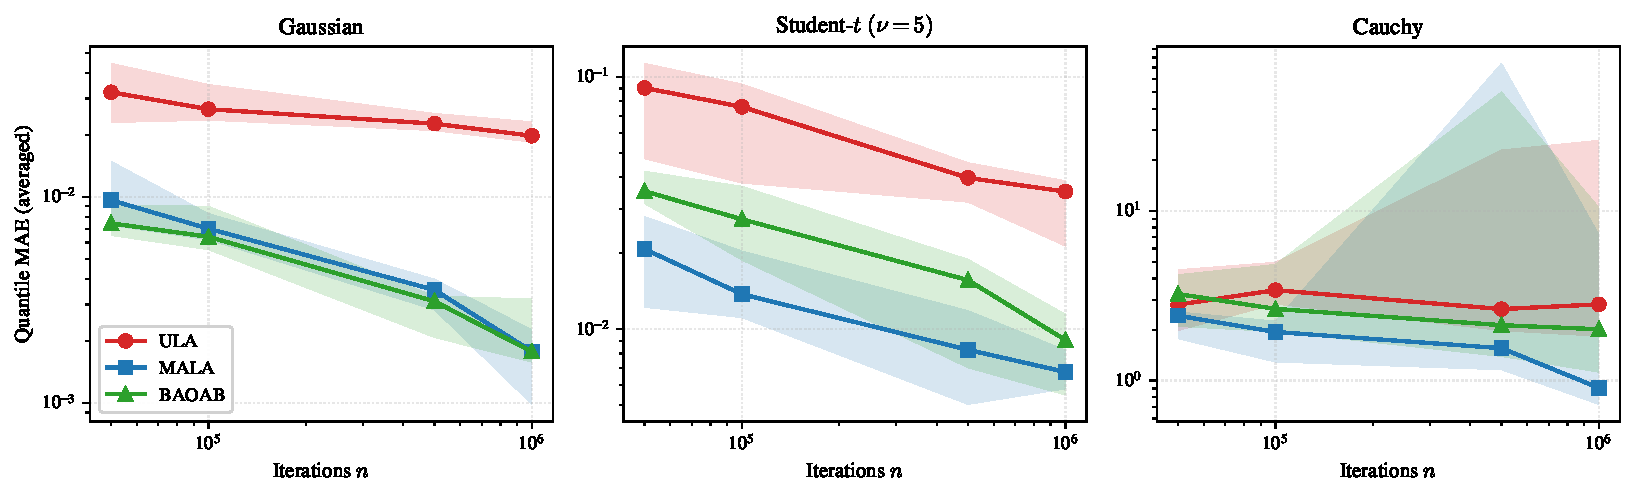
\includegraphics[width=\textwidth]{../../experiments/figures/original_thesis/quantile_mae_convergence}
\caption{Μέσο quantile MAE συναρτήσει $N$, αναπαραγόμενο από το
Σχήμα~\ref{fig:qmae-conv}.}
\label{fig:app-qmae}
\end{figure}

\subsection{Ιστόγραμμα Ποσοστών Αποδοχής Βέλτιστης Διαμόρφωσης}
\label{sec:app-fig-accept}

Το Σχήμα~\ref{fig:app-accept} (= Σχήμα~\ref{fig:mala-accept})
δείχνει πώς μεταβάλλεται το ποσοστό αποδοχής του MALA με το βήμα και τη
διάσταση. Από εδώ προκύπτει η σύσταση για ζώνη $0.5$--$0.85$ για $d \leq 10$.

\begin{figure}[ht]
\centering
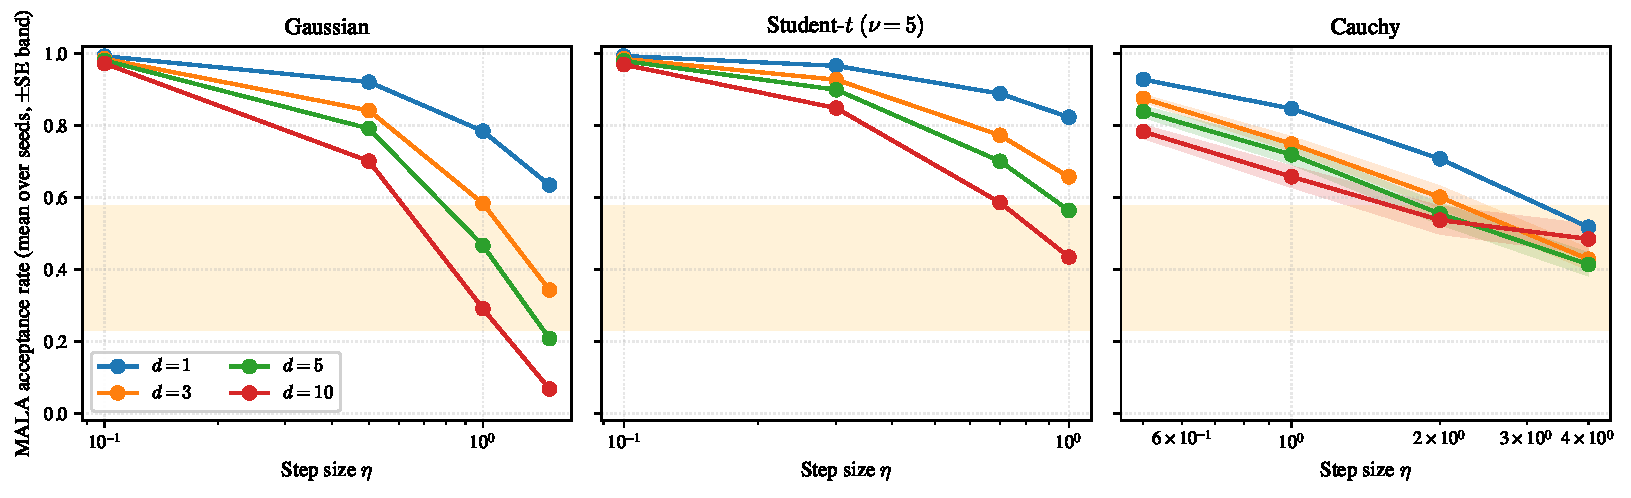
\includegraphics[width=\textwidth]{../../experiments/figures/original_thesis/mala_acceptance}
\caption{Ποσοστό αποδοχής MALA ως συνάρτηση του βήματος και της διάστασης
(επαναλαμβάνεται από την Ενότητα~\ref{sec:grid-study} για τη συζήτηση των
συμπερασμάτων).}
\label{fig:app-accept}
\end{figure}


% ---------------------------------------------------------------------------
% Βιβλιογραφία. Inline thebibliography για φορητότητα· σε οριστική διπλωματική
% θα πρέπει να αντικατασταθεί με κλήση `\bibliography{refs}` έναντι αρχείου .bib.
% Όλες οι εγγραφές είναι πραγματικές, ομότιμα αξιολογημένες αναφορές.
% ---------------------------------------------------------------------------

\begin{thebibliography}{99}

\bibitem[Andrieu and Thoms(2008)]{andrieu2008adaptive}
C.~Andrieu and J.~Thoms.
\newblock A tutorial on adaptive MCMC.
\newblock \emph{Statistics and Computing}, 18(4):343--373, 2008.

\bibitem[Andrieu and Roberts(2009)]{andrieu2009pseudomarginal}
C.~Andrieu and G.~O. Roberts.
\newblock The pseudo-marginal approach for efficient Monte Carlo
  computations.
\newblock \emph{The Annals of Statistics}, 37(2):697--725, 2009.

\bibitem[Bakry et~al.(2014)Bakry, Gentil, and Ledoux]{bakry2014analysis}
D.~Bakry, I.~Gentil, and M.~Ledoux.
\newblock \emph{Analysis and Geometry of Markov Diffusion Operators}.
\newblock Springer, 2014.

\bibitem[Cheng et~al.(2018)Cheng, Chatterji, Bartlett, and Jordan]{cheng2018underdamped}
X.~Cheng, N.~S. Chatterji, P.~L. Bartlett, and M.~I. Jordan.
\newblock Underdamped {L}angevin {MCMC}: A non-asymptotic analysis.
\newblock In \emph{Conference on Learning Theory}, pages 300--323. PMLR, 2018.

\bibitem[Dalalyan(2017)]{dalalyan2017theoretical}
A.~S. Dalalyan.
\newblock Theoretical guarantees for approximate sampling from smooth and
  log-concave densities.
\newblock \emph{Journal of the Royal Statistical Society: Series B (Statistical
  Methodology)}, 79(3):651--676, 2017.

\bibitem[Durmus and Moulines(2017)]{durmus2017nonasymptotic}
A.~Durmus and \'E.~Moulines.
\newblock Nonasymptotic convergence analysis for the unadjusted {L}angevin
  algorithm.
\newblock \emph{The Annals of Applied Probability}, 27(3):1551--1587, 2017.

\bibitem[Geyer(1992)]{geyer1992practical}
C.~J. Geyer.
\newblock Practical {M}arkov chain {M}onte {C}arlo.
\newblock \emph{Statistical Science}, 7(4):473--483, 1992.

\bibitem[Girolami and Calderhead(2011)]{girolami2011riemann}
M.~Girolami and B.~Calderhead.
\newblock Riemann manifold {L}angevin and {H}amiltonian {M}onte {C}arlo
  methods.
\newblock \emph{Journal of the Royal Statistical Society: Series B
  (Statistical Methodology)}, 73(2):123--214, 2011.

\bibitem[Jarner and Roberts(2007)]{jarner2007convergence}
S.~F. Jarner and G.~O. Roberts.
\newblock Convergence of heavy-tailed {M}onte {C}arlo {M}arkov chain
  algorithms.
\newblock \emph{Scandinavian Journal of Statistics}, 34(4):781--815, 2007.

\bibitem[Johnson and Geyer(2012)]{johnson2012variable}
L.~T. Johnson and C.~J. Geyer.
\newblock Variable transformation to obtain geometric ergodicity in the
  random-walk {M}etropolis algorithm.
\newblock \emph{The Annals of Statistics}, 40(6):3050--3076, 2012.

\bibitem[Jones(2004)]{jones2004markov}
G.~L. Jones.
\newblock On the {M}arkov chain central limit theorem.
\newblock \emph{Probability Surveys}, 1:299--320, 2004.

\bibitem[Karatzas and Shreve(1991)]{karatzas1991brownian}
I.~Karatzas and S.~E. Shreve.
\newblock \emph{Brownian Motion and Stochastic Calculus}.
\newblock Springer, 2nd edition, 1991.

\bibitem[Kloeden and Platen(1992)]{kloeden1992numerical}
P.~E. Kloeden and E.~Platen.
\newblock \emph{Numerical Solution of Stochastic Differential Equations}.
\newblock Springer, 1992.

\bibitem[Leimkuhler and Matthews(2013a)]{leimkuhler2013bao}
B.~Leimkuhler and C.~Matthews.
\newblock Robust and efficient configurational molecular sampling via
  {L}angevin dynamics.
\newblock \emph{The Journal of Chemical Physics}, 138(17):174102, 2013.

\bibitem[Leimkuhler and Matthews(2013b)]{leimkuhler2013rational}
B.~Leimkuhler and C.~Matthews.
\newblock Rational construction of stochastic numerical methods for
  molecular sampling.
\newblock \emph{Applied Mathematics Research eXpress}, 2013(1):34--56,
  2013.

\bibitem[Leimkuhler and Matthews(2015)]{leimkuhler2015molecular}
B.~Leimkuhler and C.~Matthews.
\newblock \emph{Molecular Dynamics: With Deterministic and Stochastic
  Numerical Methods}.
\newblock Springer, 2015.

\bibitem[Mattingly et~al.(2002)Mattingly, Stuart, and Higham]{mattingly2002ergodicity}
J.~C. Mattingly, A.~M. Stuart, and D.~J. Higham.
\newblock Ergodicity for {SDE}s and approximations: Locally {L}ipschitz vector
  fields and degenerate noise.
\newblock \emph{Stochastic Processes and their Applications},
  101(2):185--232, 2002.

\bibitem[Meyn and Tweedie(2009)]{meyn2009markov}
S.~Meyn and R.~L. Tweedie.
\newblock \emph{Markov Chains and Stochastic Stability}.
\newblock Cambridge University Press, 2nd edition, 2009.

\bibitem[Neal(2011)]{neal2011mcmc}
R.~M. Neal.
\newblock {MCMC} using {H}amiltonian dynamics.
\newblock In \emph{Handbook of Markov Chain Monte Carlo}, pages 113--162.
  Chapman \& Hall/CRC, 2011.

\bibitem[\O ksendal(2003)]{oksendal2003stochastic}
B.~\O ksendal.
\newblock \emph{Stochastic Differential Equations: An Introduction with
  Applications}.
\newblock Springer, 6th edition, 2003.

\bibitem[Pavliotis(2014)]{pavliotis2014stochastic}
G.~A. Pavliotis.
\newblock \emph{Stochastic Processes and Applications: Diffusion Processes,
  the {F}okker--{P}lanck and {L}angevin Equations}.
\newblock Springer, 2014.

\bibitem[Resnick(2007)]{resnick2007heavy}
S.~I. Resnick.
\newblock \emph{Heavy-Tail Phenomena: Probabilistic and Statistical
  Modeling}.
\newblock Springer, 2007.

\bibitem[Robert and Casella(2004)]{robert2004monte}
C.~P. Robert and G.~Casella.
\newblock \emph{Monte Carlo Statistical Methods}.
\newblock Springer, 2nd edition, 2004.

\bibitem[Roberts and Tweedie(1996)]{roberts1996exponential}
G.~O. Roberts and R.~L. Tweedie.
\newblock Exponential convergence of {L}angevin distributions and their
  discrete approximations.
\newblock \emph{Bernoulli}, 2(4):341--363, 1996.

\bibitem[Roberts and Rosenthal(1998)]{roberts1998optimal}
G.~O. Roberts and J.~S. Rosenthal.
\newblock Optimal scaling of discrete approximations to {L}angevin
  diffusions.
\newblock \emph{Journal of the Royal Statistical Society: Series B
  (Statistical Methodology)}, 60(1):255--268, 1998.

\bibitem[Roberts and Stramer(2001)]{roberts2001ula}
G.~O. Roberts and O.~Stramer.
\newblock Langevin diffusions and {M}etropolis-{H}astings algorithms.
\newblock \emph{Methodology and Computing in Applied Probability},
  4(4):337--357, 2001.

\bibitem[Tierney(1994)]{tierney1994markov}
L.~Tierney.
\newblock Markov chains for exploring posterior distributions.
\newblock \emph{The Annals of Statistics}, 22(4):1701--1728, 1994.

\end{thebibliography}

\end{document}
